%% BioMed_Central_Tex_Template_v1.06
%%                                      %
%  bmc_article.tex            ver: 1.06 %
%                                       %

%%IMPORTANT: do not delete the first line of this template
%%It must be present to enable the BMC Submission system to
%%recognise this template!!

%%%%%%%%%%%%%%%%%%%%%%%%%%%%%%%%%%%%%%%%%
%%                                     %%
%%  LaTeX template for BioMed Central  %%
%%     journal article submissions     %%
%%                                     %%
%%          <8 June 2012>              %%
%%                                     %%
%%                                     %%
%%%%%%%%%%%%%%%%%%%%%%%%%%%%%%%%%%%%%%%%%


%%%%%%%%%%%%%%%%%%%%%%%%%%%%%%%%%%%%%%%%%%%%%%%%%%%%%%%%%%%%%%%%%%%%%
%%                                                                 %%
%% For instructions on how to fill out this Tex template           %%
%% document please refer to Readme.html and the instructions for   %%
%% authors page on the biomed central website                      %%
%% http://www.biomedcentral.com/info/authors/                      %%
%%                                                                 %%
%% Please do not use \input{...} to include other tex files.       %%
%% Submit your LaTeX manuscript as one .tex document.              %%
%%                                                                 %%
%% All additional figures and files should be attached             %%
%% separately and not embedded in the \TeX\ document itself.       %%
%%                                                                 %%
%% BioMed Central currently use the MikTex distribution of         %%
%% TeX for Windows) of TeX and LaTeX.  This is available from      %%
%% http://www.miktex.org                                           %%
%%                                                                 %%
%%%%%%%%%%%%%%%%%%%%%%%%%%%%%%%%%%%%%%%%%%%%%%%%%%%%%%%%%%%%%%%%%%%%%

%%% additional documentclass options:
%  [doublespacing]
%  [linenumbers]   - put the line numbers on margins

%%% loading packages, author definitions

%\documentclass[twocolumn]{bmcart}% uncomment this for twocolumn layout and comment line below
\documentclass{bmcart}

%%% Load packages
\usepackage{amsthm,amsmath} %Da un error si de activa esta linea
%\RequirePackage{natbib}
\RequirePackage[authoryear]{natbib}% uncomment this for author-year bibliography
\RequirePackage{hyperref}
\usepackage[utf8]{inputenc} %unicode support
%\usepackage[applemac]{inputenc} %applemac support if unicode package fails
%\usepackage[latin1]{inputenc} %UNIX support if unicode package fails


%%%%%%%%%%%%%%%%%%%%%%%%%%%%%%%%%%%%%%%%%%%%%%%%%
%%                                             %%
%%  If you wish to display your graphics for   %%
%%  your own use using includegraphic or       %%
%%  includegraphics, then comment out the      %%
%%  following two lines of code.               %%
%%  NB: These line *must* be included when     %%
%%  submitting to BMC.                         %%
%%  All figure files must be submitted as      %%
%%  separate graphics through the BMC          %%
%%  submission process, not included in the    %%
%%  submitted article.                         %%
%%                                             %%
%%%%%%%%%%%%%%%%%%%%%%%%%%%%%%%%%%%%%%%%%%%%%%%%%


\def\includegraphic{}
\def\includegraphics{}

%%%%%%% My packages (Luis) %%%%%%%%%%%%%%%%%%%%%%%%%%%%%%%%
\usepackage{subfigure}
\usepackage{multirow}
\usepackage{hhline}
%\usepackage[markup=underlined]{changes}
%% Use "final" option to remove all tracking markups
\usepackage[final]{changes}
\definechangesauthor[color=orange]{LL}
\definechangesauthor[color=green]{JA}
\usepackage{todonotes}
\setcommentmarkup{\todo[color={authorcolor!20},size=\scriptsize]{#3: #1}}

%si se descomenta esta línea, desaparecen todos los comentarios en rojo del PDF:
%\def\release{1}
\ifx\release\undefined
\def\printcoments{1}
\fi
\ifx\printcoments\undefined
\newcommand{\todo}[1]{}
\newcommand{\nuevo}[1]{}
\newcommand{\luis}[1]{}
\newcommand{\javi}[1]{}
\else
%\newcommand{\todo}[1]{\textbf{{\textcolor{red}{TODO: #1}}}}
\newcommand{\nuevo}[1]{\textbf{{\textcolor{blue}{#1}}}}
\newcommand{\LL}[1]{\textbf{{\textcolor{orange}{#1}}}}
\newcommand{\JA}[1]{\textbf{{\textcolor{green}{#1}}}}
\fi

%%%%%%%%%%%%%%%%%%%%%%%%%%%%%%%%%%%%%%%%%%%%%%%%%%%%%%%%%%%

%%% Put your definitions there:
\startlocaldefs
\endlocaldefs


%%% Begin ...
\begin{document}

%%% Start of article front matter
\begin{frontmatter}

\begin{fmbox}
\dochead{Research}

%%%%%%%%%%%%%%%%%%%%%%%%%%%%%%%%%%%%%%%%%%%%%%
%%                                          %%
%% Enter the title of your article here     %%
%%                                          %%
%%%%%%%%%%%%%%%%%%%%%%%%%%%%%%%%%%%%%%%%%%%%%%

\title{Analysis of the cryptocurrency market applying different prototype-based clustering techniques}

%%%%%%%%%%%%%%%%%%%%%%%%%%%%%%%%%%%%%%%%%%%%%%
%%                                          %%
%% Enter the authors here                   %%
%%                                          %%
%% Specify information, if available,       %%
%% in the form:                             %%
%%   <key>={<id1>,<id2>}                    %%
%%   <key>=                                 %%
%% Comment or delete the keys which are     %%
%% not used. Repeat \author command as much %%
%% as required.                             %%
%%                                          %%
%%%%%%%%%%%%%%%%%%%%%%%%%%%%%%%%%%%%%%%%%%%%%%

\author[
   addressref={aff1},                   % id's of addresses, e.g. {aff1,aff2}
   corref={aff1},                       % id of corresponding address, if any
   noteref={n1},                        % id's of article notes, if any
   email={luislore@ucm.es}   % email address
]{\inits{LL}\fnm{Luiso} \snm{Lorenzo}}
\author[
   addressref={aff1,aff2},
   email={javier.arroyo@fdi.ucm.es}
]{\inits{JA}\fnm{Javier} \snm{Arroyo}}

%%%%%%%%%%%%%%%%%%%%%%%%%%%%%%%%%%%%%%%%%%%%%%
%%                                          %%
%% Enter the authors' addresses here        %%
%%                                          %%
%% Repeat \address commands as much as      %%
%% required.                                %%
%%                                          %%
%%%%%%%%%%%%%%%%%%%%%%%%%%%%%%%%%%%%%%%%%%%%%%

\address[id=aff1]{%                           % unique id
  \orgname{Complutense University}, % university, etc
  \street{Faculty of Statistical Studies},                     %
  %\postcode{}                                % post or zip code
  \city{Madrid},                              % city
  \cny{Spain}                                    % country
}
\address[id=aff2]{%
  \orgname{Complutense University},
  \street{Faculty of Computation Sciences},
  %\postcode{None}
  \city{Madrid},
  \cny{Spain}
}

%%%%%%%%%%%%%%%%%%%%%%%%%%%%%%%%%%%%%%%%%%%%%%
%%                                          %%
%% Enter short notes here                   %%
%%                                          %%
%% Short notes will be after addresses      %%
%% on first page.                           %%
%%                                          %%
%%%%%%%%%%%%%%%%%%%%%%%%%%%%%%%%%%%%%%%%%%%%%%

\begin{artnotes}
%\note{Sample of title note}     % note to the article
\note[id=n1]{Equal contributor} % note, connected to author
\end{artnotes}

\end{fmbox}% comment this for two column layout

%%%%%%%%%%%%%%%%%%%%%%%%%%%%%%%%%%%%%%%%%%%%%%
%%                                          %%
%% The Abstract begins here                 %%
%%                                          %%
%% Please refer to the Instructions for     %%
%% authors on http://www.biomedcentral.com  %%
%% and include the section headings         %%
%% accordingly for your article type.       %%
%%                                          %%
%%%%%%%%%%%%%%%%%%%%%%%%%%%%%%%%%%%%%%%%%%%%%%

\begin{abstractbox}

\begin{abstract} % abstract
%\parttitle{First part title} %if any
Since the appearance of Bitcoin, cryptocurrencies have experienced enormous growth not only in terms of capitalization but also in number. As a result, the cryptocurrency market can be an attractive arena for investors as it offers many possibilities, but a difficult one to understand as well. 
In this work, we aim to summarize and segment the whole cryptocurrency market in 2018 with the help of data analysis tools. We will use three different partitional clustering algorithms each of them using a different representation for cryptocurrencies, namely: yearly mean and standard deviation of the returns, distribution of returns, and time series of returns. Since each representation will provide a different and complementary perspective of the market, we will also explore the combination of the three clustering results to obtain a fine-grained analysis of the main trends of the market.
Finally, we will analyse the association of the clustering results with other descriptive features of the cryptocurrencies, including the age, technological attributes, and financial ratios derived from them. This will help to enhance the profiling of the clusters with additional insights.
As a result, this work offers a description of the market and a methodology that can be reproduced by investors that want to understand the main trends on the market and that look for cryptocurrencies with different financial performance.

\parttitle{Second part title} %if any
Text for this section.
\end{abstract}

%%%%%%%%%%%%%%%%%%%%%%%%%%%%%%%%%%%%%%%%%%%%%%
%%                                          %%
%% The keywords begin here                  %%
%%                                          %%
%% Put each keyword in separate \kwd{}.     %%
%%                                          %%
%%%%%%%%%%%%%%%%%%%%%%%%%%%%%%%%%%%%%%%%%%%%%%

\begin{keyword}
\kwd{Fintech}
\kwd{Data Sciences}
\kwd{Cryptocurrency}
\kwd{Electronic market}
\end{keyword}

% MSC classifications codes, if any
%\begin{keyword}[class=AMS]
%\kwd[Primary ]{}
%\kwd{}
%\kwd[; secondary ]{}
%\end{keyword}

\end{abstractbox}
%
%\end{fmbox}% uncomment this for twcolumn layout

\end{frontmatter}

%%%%%%%%%%%%%%%%%%%%%%%%%%%%%%%%%%%%%%%%%%%%%%
%%                                          %%
%% The Main Body begins here                %%
%%                                          %%
%% Please refer to the instructions for     %%
%% authors on:                              %%
%% http://www.biomedcentral.com/info/authors%%
%% and include the section headings         %%
%% accordingly for your article type.       %%
%%                                          %%
%% See the Results and Discussion section   %%
%% for details on how to create sub-sections%%
%%                                          %%
%% use \cite{...} to cite references        %%
%%  \cite{koon} and                         %%
%%  \cite{oreg,khar,zvai,xjon,schn,pond}    %%
%%  \nocite{smith,marg,hunn,advi,koha,mouse}%%
%%                                          %%
%%%%%%%%%%%%%%%%%%%%%%%%%%%%%%%%%%%%%%%%%%%%%%

%%%%%%%%%%%%%%%%%%%%%%%%% start of article main body
% <put your article body there>

%%%%%%%%%%%%%%%%
%% Background %%
%%
\section*{Content}
The cryptocurrency market consists of more than 4,000 cryptocoins\footnote{Although cryptoasset is a more general term, as explained in \cite{CryptoAssetsChris2018}, we will use cryptoasset, cryptocoin and cryptocurrencies terms indistinguishably in this work.} with over 800 trades per second and more than 280 exchanges. It has become a huge new market in a very short term, considering that \textit{Bitcoin} (\cite{Nakamoto2008}), first peer-to-peer and decentralised digital currency was created in 2008 and the first bitcoin was mined in 2009. While cryptocurrencies were originally intended to enable anonymous wire transfers and online purchases, they have become a powerful investment tool.

However, this new market is very diverse. Crytocurrencies with different technologies, purposes, user base coexist and form a highly heterogeneous market that is difficult to understand and to manage for those addressing a good investment allocation. 

As other assets, the value of cryptocurrencies swing based on news events, but cryptocurrencies have no physical assets or governments to back their value. Moreover, the cryptocurrency market is new, based on a still developing technology, highly speculative and small in comparison to others. As a result, it is highly volatile with big upswings, bubbles, and sudden market downturns. 

Being a market so novel, big, diverse and volatile, it needs to be understood. Several categorization efforts have been made so far. For example, the \textit{Cryptocompare} website  \footnote{\url{https://cryptocompare.com}} analyzed  over 200 cryptoassets according to regulatory aspects, level of decentralization, supply issuance, economic incentive and others. Such taxonomy is useful even if it only covers approximately the 5\% of the existing cryptocurrencies at that time. Another example is in \cite{CryptoAssetsChris2018} where classify over 200 cryptocurrencies into three classes of assets based on traditional financial markets, namely: capital asset, consumable/transformable assets and store of value asset. However, this classification is highly subjective as many times the cryptocurrencies may be a combination of some of them. Furthermore, these approaches typically cover a small fraction of the cryptocurrencies, which are the most important ones in terms of volume and popularity, and focus on qualitative aspects or aspects that do not change much. 

A different approach consists of analysing the financial performance of the cryptocurrencies and describing it from a statistical point of view. In \cite{StatisticalAnalysisOfCryptoc} analyses a few cryptocoins (Bitcoin, Dash, Dogecoin, Litecoin, MaidSafeCoin, Monero and Ripple) which exhibit heavy-tailed distributions  that fits the generalized hyperbolic distributions. In \cite{Hu2018CryptocurrenciesSF} analyses the stylized facts and return properties of 222 cryptocurrencies and find a large degree of skewness and volatility in the population of returns. Furthermore, according to \cite{Pele2020} cryptocurrencies can be clearly separated from classical assets, mainly due to their tail behaviour. However, their cluster results  also  reveal that the behaviour of the cryptocurrencies is diverse. 

The same conclusion can be drawn in other clustering analysis using cryptocurrencies. In \cite{Stosic2018CollectiveBO} is represented the correlations of 119 cryptocurrencymarket as a complex network and discover distinct community structures in its minimum spanning tree. In \cite{Song2019} analyses 76 cryptocurrencies using the correlation-based clustering and filtering out the linear influences of Bitcoin and Ethereum and detect 6 clusters, but that do not remain stable after the announcement of regulations from various countries. The time dimension plays an important role in the work in \cite{HigorSigakiClusteringPattersCrypto2018}, that cluster the time series of 437 cryptocurrencies using hierarchical clustering and detect 4 different groups where the behaviour evolves differently in terms of efficiency for the information.

All these approaches reveal that it is possible to establish  different groups of cryptocurrencies in terms of their financial performance. And identifying them, it is useful to better understand the cryptocurrency market, but also for building a diversified  portfolio. 

All of these methods use different representations of the cryptocurrencies: correlations in \cite{Stosic2018CollectiveBO, Song2019}, factors extracted from the correlation matrix  (\cite{Pele2020}) and time series (\cite{HigorSigakiClusteringPattersCrypto2018}) . Each representation focuses on different aspects of the cryptocurrency that are meaningful for the purpose of the analysis. 

However, it would be possible to combine the clustering results using different representations of the cryptocurrencies where each one take into account different aspects of the cryptocurrencies. In this way, the combination of the clustering results would make possible to characterize each cryptocurrency in several dimensions, one for each cluster strategy. If the clusters for each cluster strategy are meaningful, their combination would offer a more detailed characterization of the market and useful insights for portfolio management.

In this work, we will explore the combination of clustering of cryptocurrencies using  \cite{R_opensourcelanguage}. We will go beyond a few hundreds cryptocurrencies, as most studies do, and will explore all the cryptocurrencies traded in 2018 (more than 1,700 cryptocurrencies) easily scalable for a growing market. We will describe each cryptocurrency considering the log return transformation of the daily price  in 2018 with three different levels of granularity: 

\begin{itemize}
	\item Mean and standard deviation of the daily returns
	\item Distribution of the daily returns
	\item Time-series of the daily returns 
\end{itemize}

In the first case, we provide a meaningful summary commonly used to describe financial assets over time as it is the annualized return and volatility, or with the central tendency and the  dispersion of the returns. In the second case, we consider the whole distribution of returns that accounts not only for the central tendency and dispersion of an asset, but for the whole aggregated behaviour including asymmetry, kurtosis and the tails. Methods to analyse distributional data belong to the field of symbolic data analysis (\cite{NoirhommeBrito2011}), where observations account for internal variation that can be represented as intervals or distributions, and have been previously used in finance (\cite{Arroyo2009, Arroyo2011, GONZALEZRIVERA2012}). Finally, we  consider the observed data, that is the log return time series that accounts for variations over time and makes possible to identify when volatile or stable periods take place in each cryptocurrency. 

There is a high diversity of clustering techniques, but in our case the interest lies on the different perspectives shown at each level of granularity. Thus, for all the representations we will use a partitional prototype-based clustering algorithms with a similarity measure (distance) meaningful for each kind of representation. In this way, we will have a prototype describing the behaviour of each cluster using the same representation of the data. Prototypes make possible to assign a financial meaning to the whole cluster. 

Then, we will combine the three clustering results and analyse the most numerous intersections with the help of visual tools. Such approaches are successfully used in biostatistics (\cite{l2015xclusim, kern2017interactive}). In our case, we will use them to represent the main trends in the cryptocurrency market. If several cryptocurrencies belong to the same clusters in the three clustering results then we can consider them as very similar. We will inspect the relationship among the three clustering results with the help of visualization tools. 

This approach provides a screening mechanism that allows us a meaningful exploration of the whole market in spite of its complexity and size. The intersection of the clustering results can also be helpful for investors in order to select a suitable cryptocurrency for the portfolio as it characterizes the cryptocurrency market in more detail.

In a further step, we will investigate the association between the clustering results and different features of the cryptocurrencies such as technological variables, the market capitalization, the \textit{maturity} (age) of the cryptocurrency, and some of asset portfolio ratios. We aim to inspect whether some clusters are tightly associated or not with some aspects not taken into account the clustering process. we apply some inference statistical tests to assess whether associations are significant. These associations enhance the profiling of the different clusters. We keep continuous references to concrete cryptocurrencies of the market, most of them no very known,  that are part of our analysis. Finally, we present our conclusions with some points open to debate. 


\subsection*{Related work}

\subsubsection*{Clustering financial data}

Clustering analysis is a well-known data analysis tool that have served well in different fields  (\cite{ClusterAnalysisHandBookCRCPress2016}). In particular in Finance, the seminal work of  \cite{HierarchicalStructureFinancialMK1999} used the cross-correlation of the return time series and Minimum Spanning Trees (MST) to group the stocks of the New York Stock Exchange from 1989 to 1995. In \cite{HierarchicalStructureFinancialMK1999} is applied the MST to represent the stock market as a network. Later, in \cite{Bonanno_2004} applies the same methodology considering different time horizons comparing the return and volatility networks. The methodology of Mantegna is applied with different variations in other contexts (\cite{Onnela2_2003, Mizuno_2006, BridaRisso2010}). Furthermore, different alternatives and variants of this methodology have been proposed as it can be seen in the review in \cite{Gautier2017} 

Another strand of clustering applied partitional methods as we do but more specifically fuzzy-types to financial markets typically used for grouping stocks for developing portfolios. In \cite{Nanda2010ClusteringIS} applies K-means, Fuzzy C-means  and Self Organizing Maps (SOM) to returns and financial ratios from Indian stocks to  classify  them in  different clusters  and  subsequently  develop  portfolios  from  these cluster. A derivate approach is shown in \cite{Tamal2015}, who group the daily Indian market volatility comparing Kernel K-means, SOM and Gaussian clustering models to achieve right volatility prediction using the clusters as predictors. In the same way, \added[id=LL,comment={new cites}]{\cite{PierpaoloDUrso2013},\cite{PierpaoloDUrso2016} and \cite{PierpaoloDUrso2020}} applied different variations of fuzzy clusters to financial markets. \added[id=LL,comment={reviewer 1}]{Our methodology requires fully distinguished classes for the clustering objects, partial membership of \textit{fuzzy} clusters is more complicated to handle with our approach so a pure crisp partitions is preferred for the methodology proposed.}

In \cite{Liao2007MarketClustering, Liao2013TaiwanChinaStocks5} do clustering on the daily market data and apply different association rules between the K-means groups, indices and market categories. That associations help to analyse and describe the co-movement among the different markets.

Regarding the use of time series as objects to cluster, in \cite{Aghabozorhi2013ThreePhases} propose a three-phase clustering model to categorize companies based on the similarity in the shape of their stock markets using Dynamic Time Warping (DTW) (\cite{DisimilDTW1994}). 

\subsubsection*{From  traditional finance to cryptoasset markets}

In \cite{NBER2013} analyses Bitcoin market in-depth and considered it an investment more speculative than a currency.It is considered that it poses high risk for the management of transactions and credit markets. Finally, a deflationary scenario is anticipated because of the limited number of bitcoins that can be issued (21 millions). The paper anticipated many aspects of the cryptocurrency markets that we are experiencing today (excessive volatility, high level of computer knowledge required for using and integration into the web of international payments).

The high growth of the cryptocurrency market and its heterogeneity since 2014 was analysed in depth in \cite{SystematicAnalysisCrypto2018} considering different aspects including regulatory, cyber-criminality, market efficiency or bubble dynamics and make recommendations for further investigations on different domains. We take a couple of them and we address in our work some characteristics based on liquidity (market cap) and other key market metrics, for instance, Beta or Modigliani-Modigliani  financial ratios. 


The characterization of the cryptocurrencies from a statistical point of view has been tackled by different works. In \cite{StatisticalAnalysisOfCryptoc} analyses the distributions for a few cryptocurrencies (Bitcoin, Dash, Dogecoin, Litecoin, MaidSafeCoin, Monero and Ripple) and show that they exhibit heavy-tailed distributions  that fit the generalized hyperbolic distributions. As part of a benchmark with other markets, in \cite{baek2015bitcoins} shows that the volatility of Bitcoin market shows that bitcoins are 26 times more volatile than S\&P 500 Index.  

In \cite{Zhang2018SomeSF} analyses the stylized facts of eight cryptocurrencies that represent almost 70\% of the market capitalization and find, among other things, heavy tails for the returns, return autocorrelations that decay quickly, while the autocorrelations for absolute returns decay slowly, that returns display strong volatility clustering and leverage effects, and a power-law correlation between price and volume. The study of stylized facts have been extended  increasing  the number of digital coins up to 222 \cite{Hu2018CryptocurrenciesSF}.


\subsubsection*{Clustering of cryptocurrencies}

The classical methodology based on MST algorithms (\cite{HierarchicalStructureFinancialMK1999}) is applied in \cite{Song2019} to filtering the influence of \textit{Bitcoins} and \textit{Ethereum} and detects six homogeneous clusters. However, the structure found does not remain stable after the announcement of regulations from various countries. Interestingly, the  uses of clustering together with other methods, such as VAR models and Granger causality tests (\cite{ShockTransmissionCryptoMK2019}) help to find that Bitcoin shock prices are not transmitted to the prices of other cryptocurrencies, being \textit{Litecoin} and \textit{Dogecoin} the more influential actors. According to the results, Bitcoin exhibits a lower relationship with other cryptocurrencies. Other approach is the use of random matrix theory and hierarchical structures in a MST on 119 cryptocurrencies from 2016 to 2018 (\cite{Stosic2018CollectiveBO}). It is showed that the  presence of multiple collective behaviours in the market of cryptocurrencies, which contrast to the intuitive idea that Bitcoin exerts a global influence on the entire market.

Furthermore, the time dimension can also be taken into account evolve. In \cite{HigorSigakiClusteringPattersCrypto2018}  first classify 437 cryptocurrencies according to information efficiency using permutation entropy and statistical complexity, and then cluster their time series using dynamic time warping and hierarchical clustering to find four groups where the behaviour in terms of information efficiency evolves differently. All these articles evidence the complexity of the underlying structure in the cryptocurrency market, where some cryptocurrencies influence others even in unexpected ways. 

The comparative study of  cryptocurrency markets and traditional financial markets is also an essential domain of investigations. In \cite{CryptoDynamicRelationships2018} shows that cryptocurrencies are highly connected among themselves and disconnected from mainstream assets (bonds, stocks, S\&P500, gold).In \cite{Pele2020} merge classification based on asset profiles and dynamic evolution of clusters. It starts with a characterization of selected group of log-returns assets including 150 cryptocurrencies, stocks commodities and exchange rates to estimate a multidimensional vector applying a dimension reduction (Factor analysis). Then, they use  classification where K-means is one of the techniques applied. The main difference of Cryptocurrencies with respect to traditional assets is a higher variance and longer tails of the log-return's distribution. The work also shows that individual cryptocurrencies tend to develop over time similar characteristics (synchronic evolution).\added[id=LL,comment={new cites}]{\cite{Dro_d_2019}shows that the multiscaling characteristics of the exchange rate fluctuations comparing the cryptocurrency market approach to those of the Forex; furthermore \cite{BEGUSIC2018400} estimates the scaling exponent and find the asymptotic power-law behaviour for Bitcoin.}


\section*{Methodology}
\subsection*{Dataset preparation}
We retrieved data from \url{https://www.cryptocompare.com/} for all the cryptocurrencies traded during 2018. New cryptocurrencies have appeared in the last years, but many of them were short-lived and barely traded. \added[id=LL,comment={answer to reviewer 3}]{We aim to incorporate in our descriptive estudy as many cryptpcourrencies as possible on the market during the period which means that we are very conservative on the \textit{clearing data} criteria, we only removed NaN and Inf observations mainly caused by zero-prices in log transformations}. As  result, from all the downloaded cryptocurrencies we filtered out those that were in the market less than the 95\% of the days (92 cryptocurrencies in 2018), but we kept some that were in the market but were not traded, i.e. zero return and volatility or zero volume. Our final data set consists of 1,723 cryptocurrencies. \added[id=LL,comment={reviewer 3 suggested to analyse the volume of trading}]{Anyway, part of the cryptocurrencies present a very low activity in the market point to low liquidity that cause heavy-tails effect so for that case we apply a specific \textit{filter} in some parts of the study, mainly for association tests}

For these cryptocurrencies we constructed the following variables:


\begin{itemize}
	\item \textbf{Daily log-returns}: The use of returns instead of prices in Finance price time-series is very extended and consolidated due to its more suitable statistical properties and better comparability. It has been used in cryptocurrency markets as well \cite{CryptoCurrencyDrives, Stosic2018CollectiveBO}. The  return for the cryptocurrency $i$ at day $t$s is computed as:
	$$
	r_i(t)=ln(P_i(t))-ln(P_i(t-1))
	$$
	where $P_i(t)$ is the daily cryptocurrency price for $i$ cryptoasset at day $t$. 
	
	\item \deleted[id=LL]{Market cap} \added[id=LL,comment={reviewers 2}]{\textbf{Volume}}: It is the  \deleted[id=LL]{one-year average} daily traded volume in units of the base cryptocurrency \deleted[id=LL]{in dollars} \added[id=LL]{that can be understood as a liquidity proxy}. We transformed it into an ordinal variable by the quantile functions. Three cryptocurrencies represent 66\% of the trading volume of the market in 2018, namely Bitcoin (46\%), Ethereum (16.5\%) and EOS (4\%), and in total 10 cryptocurrencies (\texttt{BTC, ETH, EOS, BCH, XRP, LTC, ICX, HSR, ETC, IOT}) represent 80\% of the daily volume.
	
	\item \added[id=LL,comment={}]{\textbf{Market cap}: it is the one-day market cap retrieved directly from the market on the 4th of February in 2019. Three cryptocurrencies represent 60\% of the \textit{market cap}, namely \texttt{WBTC*} (26.8\%), \texttt{BTC}(22.4\%) and \texttt{NPC} (11.5\%)}, and in total 5 cryptocurrencies (\texttt{WBTC*, BTC, NPC, XRP, AMIS}) represent 80\% of the \textit{market cap}
	
	\item \textbf{Technological variables}: We represent the encryption and consensus algorithms of the cryptocurrency as nominal variables:
	\begin{itemize}\itemsep0.5pt
		\item \textbf{Encryption}: There are 105 different values. The more relevant encryption algorithms are Scrypt, SHA256, SHA256D, X11, X13, X15, PoS, Multiple and CryptoNight. We notice that this information is not available for 35\% of the cryptocurrencies (599 obs.). 
		\item \textbf{Consensus}: There are 60 possible values, including the well known Proof of work (PoW) and Proof of Stake (PoS). The most predominant are obviously PoW/PoS, PoW and PoS but this information is missing in 31\% of the cryptocurrencies (536 obs.)
	\end{itemize}  
	\item  \textbf{Age}: We estimate the time on the market of each cryptocurrency, and transform it into an ordinal variable by a quantile function. \textit{Age} and \textit{maturity} are interchangeable on our study. 
\end{itemize}

Besides the cryptocurrency data, we also retrieve time-series from  \added[id=LL,comment={reviewers 2 and 3}]{https://cci30.com/ which is a rules-based index designed to objectively measure the overall growth, daily and long-term movement of the blockchain sector} and the US Department of the Treasury\footnote{\url{https://home.treasury.gov/}} that we use for the computation of some financial benchmarking rates as Beta, Sharpe ratio and others that we will explain in the next sections.\\ 


\subsubsection*{Volume of negotiation and tail distribution analysis}
\added[id=LL,comment={Reviewer 3}]{
 We aim to consider all cryptocurrencies that existed on the market independently of the transaction volume or liquidity. For sure liquidity or volume of trading is a key aspect to keep in mind to characterize the market but our first priority is to represent and manage all the market. We represent a histogram of non-trading days based on the volume negotiated (volume equal to zero means in our case no traded asset) on Figure \ref{fig:TradingDays} where 306 cryptocurrencies has been traded (volume of negotiation equal to zero) no day during 2018 (18 crypto currencies traded only 2 days). As we commented, we consider relevant to keep non-traded cryptocurrencies as part of our market analysis for the clustering part just to detect where they are allocated. However, we agree on the low interest for the investor in lower liquidity crypto assets.\\
}

\added[id=LL,comment={Reviewer 3}]{The concept of power-law distribution \cite{Newman2005power} and applications on cryptocurrency case \cite{BEGUSIC2018400}, \cite{WATOREK2020} is relevant to confirm the existence of 1st and 2nd order moments on our data to ensure the applicability and generalization of the results of clustering and the inference tests. The existence of the statistic moments according to the power-law \cite{poweRlaw} is:}


\begin{equation}
	p(x) = \frac{\alpha-1}{x_{min}} \left(\frac{x}{x_{min}} \right)^{-\alpha},
\end{equation}


and for the CDF
\begin{equation}
	P(X \leq x) = 1-\left(\frac{x}{x_{min}}\right )^{-\alpha + 1},
\end{equation}


\added[id=LL,comment={Reviewer 3}]{The moments of the power law distribution for the continous power law are the following:}

\begin{equation}
	E\left[X^m \right]= \int_{x_{min}}^{\infty}x^mp(x)\cdot dx = \frac{\alpha - 1}{\alpha-1-m}x_{min}^m
\end{equation}


Generally speaking when
\begin{itemize}
	\item $1 \le \alpha \leq 2$, all moments diverge, i.e., $E[X]=\infty$;
	\item $2 \le \alpha \leq 3$, all second and higher-order moments diverge, i.e., $E[X^2]=\infty$;
	\item $3 \le \alpha \leq m+1$, all m and higher-order moments diverge, i.e., $E[X^m]=\infty$;
\end{itemize}


	
\cite{Newman2005power} showed that for the case $2 \le \alpha \leq 3$ as $X_{max}$ becomes large we get that
\begin{equation}
	E\left( x^2 \right) \sim n^{(3-\alpha)/(\alpha-1)}
\end{equation}
converge. In \ref{tab:ListCryptoPart1}, \ref{tab:ListCryptoPart2}, \ref{tab:ListCryptoPart3}, \ref{tab:ListCryptoPart4} and \ref{tab:ListCryptoPart5} we have computed the maximum likelihood estimator (MLE) for the continous power law for the negative and positive tails on the variables \texttt{AlphaP} and \texttt{AlphaN}  as follows:
\begin{equation}
	\hat{\alpha} = 1 + n\left[ \sum_{i=1}^{n}\log \frac{x_i}{x_{min}} \right]^{-1}
\end{equation}
with the following expected statistical error (variables \texttt{Sd.P, Sd.N} for positive and negative tails on the table \ref{tab:ListCryptoPart1})
\begin{equation}
	\sigma = \sqrt{n}\left[ \sum_{i=1}^{n}\log\frac{x_i}{x_{min}} \right]^{-1} = \frac{\alpha-1}{\sqrt{n}}
\end{equation}


\added[id=LL,comment={Reviewer 3}]{In our view, we consider that power-law behaviour could be more impacting on the generalization of the inference tests than clustering partitions. Our goal is to represent all the cryptocurrency market on a clustering maps independetly of any statistical property or behaviour considering them as objects and in that way we keep the 1723 cryptocurrencies for clustering.In other words, we want to know where are allocated the highest \textit{heavy-tail} cryptocurrencies as well. For association tests our goal is the generalization of the results and in that way we filtered out the lsit of cryptocurrencies keeping only the higher statistic quality, 1262 cryptocurrencies in total.}

\subsection*{Methods}

We aim to find groups of cryptocurrencies based on the behaviour of their log-returns in 2018 and describe them. For such purpose we will use different clustering algorithms that will deal with the three representations of the log-returns described in the previous section:  statistic moments, observed probability distribution and observed daily time-series.

We use centroid-based clustering algorithms because the centroids provide us an interpretable summary of the elements of each cluster, which will help us to identify the most relevant features of the cluster elements. A drawback in this type of clustering algorithms is that they assume knowledge about the desired number of clusters ($k$). We apply different quality criteria to determine the optimum number of clusters depending on the technique.

Moreover, we use distance-based clustering algorithms they are simple, intuitive and applicable for a wide variety of scenarios \cite{DataClusteringAlgorithms2014}. The algorithms considered will be based on meaningful dissimilarity measures or distances that help on the interpretability of the clusters. That is especially important for more complex representations such as the distributions or the time series. For example, in the case of distributions, the measure should relate with properties of the density function (central tendency, spread, symmetry), while in the case of time series will be more with the shape of the time series along time. Meaningful measures will help us to understand better the resulting clusters and to interpret the nearness of the observations to the centroid. In addition, our clustering algorithm provide a prototype or a centroid of the clustering, which eases the characterization of the resulting clusters. 


The cluster intersections help us to merge the results of the different clusters and identify the most prominent cryptocurrency profiles along 2018 according to different characteristics through the three techniques. Furthermore, we analyse the association between the clustering results found for the three representations and the different attributes of the cryptocurrencies. 

\subsubsection*{The k-means clustering algorithm for the first and second statistical moments}

For the bi-variate (or two-moments) representation, where the two variables are  the yearly mean and standard deviation of the log-returns we use the k-means clustering \cite{KmeansMacQueen1967}, which is one of the most widely used clustering algorithms \cite{Wu2008Top10Alg}. We standardize the two variables to homogenize the differences between their ranges. The K-means clustering minimizes within-cluster variances, that is, squared Euclidean distances inour case, which makes the result easy to understand and interpret. Before the clustering, we compute the Hopkins statistic \cite{Banerjee2004ValidatingCU} to rule out the possibility that a uniform random distribution generated the data set. 

For the selection of the number of clusters (k) we compute several internal Cluster Validity Indices (CVIs) for crisp partitions \cite{Arbelaitz2013AnEC}, including silhouette, Dunn, COP Davies-Bouldin, Calinski-Harabasz or the score function, and then apply the majority rule to choose the best number of clusters.

We apply clustering ensemble techniques \cite{Ghosh2011} aiming at reducing the randomness on the partitional cluster results. We run the K-means algorithms 10 times and we ensemble the outcomes minimizing the Euclidean distance. We confirm that the dissimilarity among the different runs is closer to zero, which makes the ensemble cluster a more stable representation. For each algorithm run, we apply the Hartigan-Wong method for clustering \cite{HartiganWong1979} with ten iterations to reach convergence and considering 50 random starts for each iteration. Once we have the 10 algorithm runs, we compute the medoid of an ensemble of partitions, i.e, the element of the ensemble minimizing the sum of dissimilarities to all other elements \cite{Clue2019,Clue2019Rpackage}.


\subsubsection*{The dynamic histogram clustering for the log-return distribution}

For the yearly log-return distribution, we apply a clustering algorithm that deals with histogram-data form. More precisely, we apply the dynamic clustering algorithm for histogram data based on the $\mathit{l}_2$ Wasserstein distance  \cite{Irpino2006, HistogramClust2013}. In this way, we will group the cryptocurrencies with similar distributions of log-returns in 2018.

The dynamic clustering algorithm needs a dissimilarity function to assign the observations to the clusters, which is the $\mathit{l}_2$ Wasserstein distance. Given two histograms $h_1$ and $h_2$, the  $\mathit{l}_2$ Wasserstein distance is defined as

\begin{equation}
	d_W(h_1,h_{2}):=\sqrt{\int_{0}^{1}\left[F_1^{-1}(t)-F_{2}^{-1}(t)\right]^2dt}
\end{equation}
where $F_1^{-1}$ and $F_{2}^{-1}$ are the inverse of the cumulative distribution functions, that's the quantile functions of $h_1$ and $h_2$, respectively. This distance can be decomposed as follows: 
\begin{equation}
	d_W(h_1,h_{2})=\sqrt{\left(\mu_1-\mu_{2}\right)^2 + \left(\sigma_1-\sigma_{2}\right)^2+2\sigma_1\sigma_{2}\left(1-\rho_{1,2}\right)}
\end{equation}where $\mu_i$ and $\sigma_i$ are respectively the mean and the standard deviation of the $h_i$ and $\rho_{1,2}$ is the correlation of $h_1$ and $h_2$ \cite{Irpino2015BasicSF}. As a result, the $\mathit{l}_2$ Wasserstein distance can be decomposed in the addition of three elements that account for the histogram differences in terms of location, spread and shape, respectively. Interestingly, this distance matches the perceptual similarity that the human observes when comparing distributions \cite{Arroyo2009}. All these aspects make it a suitable distance for clustering distributions and, in our case, log-return distributions.

The Dynamic Clustering Algorithm for histogram data based on the Wasserstein distance (Hist DAWass) is a k-means-like algorithm for clustering a set of observations described by histogram variables \cite{Irpino2006, HistogramClust2013}. Each of the $k$ clusters is represented by a centroid or prototype and observations are assigned to the closest prototype. The prototype is the average histogram of the observed histograms for each variable. In our case, observations are described by a single histogram variable representing the distribution of log-returns and the resulting prototype is a histogram that averages the histograms of the observations that belong to the cluster \cite{Irpino2015BasicSF}. As a result, the prototypes can be interpreted in a financial context as log-return distributions.

We use the clustering implementation in the R-package HistDAWass \cite{Irpino2016}. This implementation provides quality measure that is the percentage of Sum of Squared (SS) deviation explained by the model running the algorithm several times for each $k$. We run the clustering algorithm 20 times for each $k$ and the solution is the best one among the repetitions, that is, the one that maximizes the SS. 

\subsubsection*{The TADPole clustering for the log-return time-series}

Time-series clustering is a challenging domain for clustering due to the high dimensionality of the objects and how they are ordered. As a result, many approaches have bee proposed over time \cite{Liao2005Clustering,Rani2012RecentTO, Aghabozorgi2015TSClust}. 

We wish to cluster the time-series with similar volatility patterns in the same periods. For this purpose, Euclidean distance may fail to produce an intuitively correct measure of similarity between  two  time series, because it  is  very sensitive  to  small  distortions in the time  axis. However, other measures, such as Dynamic Time Warping (DTW), cope with this problem by \textit{warping} non-linearly the time dimension to estimate their similarity. Nowadays, DTW is considered one of the most popular and useful shape-based measures \cite{Aghabozorgi2015TSClust}.

However, DTW is intrinsically slow because of its quadratic time complexity, which hampers its applicability in clustering. Thus, we use the TADPole (Time-series Anytime Density Peak) \cite{TADPole2015}  clustering algorithm that extends the Density Peak (DP) clustering framework \cite{Rodriguez1492} and exploits the upper and lower bounds of DTW to prune unnecessary distance computations which speed-up the convergence of the algorithm. As a result, TADPole produces a right answer quickly, and then refines it until it converges to the exact answer. Besides, the clustering algorithm only needs two parameters which makes it easy to use. Firstly a cut-off distance that define the thresholds to select the series and we set it to 2; and secondly,  a windows-size that define the time frame to make the comparison between the series that we set to 3. Optionally we can also  select the number of clusters ($k$) or we can let the algorithm to choose the optimal one based on the local density of points (closer series at some time based on some cut-off distance) using a “knee point finding” algorithm where points with higher values of $\rho_i \cdot \delta_i$, where $\rho_i$ referred to the local density and $\delta_i$ is the distance from points with higher local density.

We will consider a different number of clusters $k$ and compute the internal Cluster Validity Index (CVI) for each of them. As this clustering algorithm uses three distances, we used as CVI the Calinski-Harabasz index that secure the convergence of the algorithm for asymmetric distance measure.

TADPole allows to cluster time-series with arbitrary shapes which is very useful in our case because of the heterogeneity  of the cryptocurrency market. In contrast, TADPole clusters cannot be represented as "balls"  in a metric plane as in K-means for example. The result is a Partition Around Medoid (PAM) type centroid using the DTW distance that can be represented in a \textit{DTW} space. This centroid is a time-series that serves us to identify the volatility patterns of the resulting clusters.

We apply the R implementation of TADPole algorithm in the R-libraries \cite{DTWCLUST, DTWCLUST2}. The time series is on  log-return values which facilitate the characterization of the clusters. The DTW measure implemented in the package follows the estimation by \cite{Lemire2008}. 

\subsubsection*{Combination of clustering results}\label{sub:ClusteringEnsem}

Once we have the results of the clustering algorithms, we combine them by intersecting the clusters. Potentially we have $T_1 x T_2 x T_3$ intersections where $T_n$ is the number of clusters that we obtain with the clustering algorithm $n$.
The combination of the clustering results would make possible to characterize each cryptocurrency in several dimensions, one for each cluster strategy. The resulting multi-dimensional categorical datasets can be shown  using visualization techniques supported on the graph theory \cite{l2015xclusim, kern2017interactive}. To better highlight the changes in the clustering between the different techniques, we have visualized such changes by means of a so called alluvial diagram \cite{Rosvall2010MappingCI}. We use the alluvial visualization  implemented in R-library \cite{alluvial2016} to show the main \textit{flows} of cryptocurrencies.

We will analyse the clustering intersections with the higher cardinality to better profile the main trends of the cryptocurrency market.


\subsubsection*{Association test}

Finally, we complement the information of each cluster result by studying the level of association with different independent variables not considered in the clustering process. We analyze the association among clusters and the categorical variables defined in Table \ref{tab:CatVar} by applying the exact Fisher's tests and analysing the Person's residuals of the contingency tables that we explain later. Firstly, we transform quantitative variables into ordinal by applying the quantile functions.\\

We introduce below some variables that are financial ratios \cite{bacon2008practical} that we borrow from portfolio theory and we use to characterize the behaviour of the cryptocurrencies from a investor perspective, enhancing the association study as well. The computation of most of the below ratios (except Beta that has been manually computed) rely on the ratios implemented on R-library \cite{PerformanceAnalytics}. 

\textbf{Beta} is a volatility measure of systematic risk of an asset, the risk inherent to the entire market that is non-diversifiable, in statistic terms, \textit{beta} is the slope of the regression of our asset compared with a reference on the market:
\begin{equation}
	\beta = \frac{Cov(R_c,R_b)}{Var(R_b)}, 
\end{equation}
where $R_c$ is the return of our cryptocurrency, $R_b$ is the return of the bench market, \deleted[id=LL] {NASDAQ Composite} \added[id=LL,comment={Reviewer 2,3}]{the CCI30 index that track the 30 largest cryptocurrencies by market capitalization, excluding stablecoins}. \deleted[id=LL]{We choose the NASDAQ instead of the more usual S\&P500, because NASDAQ is a market whose behaviour should be closer to the cryptocurrency markets than S\&P500, being a technological index as well as cryptocurrency market}. The \textit{beta} value shows whether an asset  moves in the same direction as the reference index, and how volatile or risky is compared with it. The Beta for the whole market is 1.0. A positive beta means the asset moves in the same direction as the market, while negative beta means that the asset moves in opposite direction. Furthermore, an absolute value greater than 1 means greater sensitivity to systematic risk, i.e. higher risk; while values lower than 1 mean less sensitivity. 

The \textbf{Sharpe ratio}(Sharpe variable)  is the exceed average return of risk-free by volatility unit or total risk. The ratio  determines the risk of the investment with respect to the return of an investment with zero-risk:
\begin{equation}
	\label{eq: Sharp}
	SR_c =\frac{E[R_{c}-R_{f}]}{\sigma_c},
\end{equation}
where $R_c$ is the return of our cryptocurrency,  $\sigma_c$ is standard deviation or the volatility of our cryptocurrency and $R_f$ is the \textit{risk-free} rate taken as reference; we considered the daily of the annualized T-Bill over 90 days, and its daily value for 2018 was \added[id=LL,comment={corrected value}]{$E[R_f]=0,005254377\%$} . The greater the value of the Sharpe ratio, the more attractive the risk-adjusted return of the cryptocurrency.

\deleted[id=LL]{The \textbf{Modigliani-Modigliani ratio} (M2 variable) is a risk-adjusted return that makes easier the comparison of different returns computed at different risk levels. We can see it as an extension of Sharpe ratio}

%\begin{equation}
%	\label{eq: M2}
%	MM_c=SR_{c}\sigma_b + E[R_f],
%\end{equation}

\deleted[id=LL]{where $SR_c$ is the Sharpe ratio of our cryptocurrency as defined in equation \ref{eq: Sharp}, $E[R_f]$ is the risk-free rate in 2018 and $\sigma_b$ is the standard deviation of the benchmark market, NASDAQ composite in our case.
The \textbf{Sortino ratio} (Sort variable) is defined as follows}
%\begin{equation}
%	\label{eq: Sort}
%	Sort_c  = \frac{E[R_{c}-R_T]}{\sigma_D},
%\end{equation}
\deleted[id=LL]{where $\sigma_D$ is the downside risk, which measures the variability or standard deviation of negative returns below a minimum
target rate $R_T$ and assumes that the cryptoasset returns decline in certain period of time} 
%\begin{equation}
%	\label{eq: downside risk}
%	\sigma_D = \sqrt{\sum_{i=1}^n{\frac{min((R_c - R_T),0)^2}{n}}},
%\end{equation}
\deleted[id=LL]{being $R_T$ the \textit{minimum acceptable return} that in our case is the \textit{risk-free return} $R_f$ in 2018. All returns higher than the threshold $R_T$ are counted as zero in the calculation of the semi-standard deviation.
The \textbf{M squared for Sortino} (M2Sort variable) is a Modigliani-Modigliani ratio, as defined in equation \ref{eq: M2} adjusted for downside risk instead of total risk}
%\begin{equation}
%	\label{eq: MS2}
%	M_S^2 = R_c + Sort_c * (\sigma_{Db} - \sigma_D),
%\end{equation}

\deleted[id=LL]{where $Sort_c$ is the Sortino ratio of our cryptocurrency,  $\sigma_{Db}$ is the benchmark annualized downside standard deviation or risk and $\sigma_D$ is the cryptoasset annualized downside risk, as defined in equation \ref{eq: downside risk}. The benchmark index for this ratio is the NASDAQ Composite.}

Typically, \textbf{Chi-Square test} is used to examine the significance of the association between categorical data on a contingency table. However,the significance value is an approximation that it is not adequate when the sample size is small. We ruled out the Chi-Square test since results are not significant if the expected frequency is not typically higher than 5 in at least 80\% of the cells of the contingency table (\cite{ContingencyTable1984}) and this assumption is not fulfilled in our case for many of the categorical variables for some levels. we will use
the Fisher's exact test (\cite{ContingencyTableFisher1922}) to test the association between the variables of the Table \ref{tab:CatVar} and the cluster results, which is applicable for all sample sizes. This test assumes no dependency between the categorical variables as null hypothesis, and assumes a multivariate hyper-geometric distribution for the cells into the contingency tables (\cite{Mehta1983ANA}).

For large datasets Monte Carlo method provides an unbiased estimate of the exact  \textit{p-value} (\cite{mehta1996exact}). Monte Carlo is a repeated sampling method that for any observed table, there are many tables, each with the same dimensions and columns and row margins as the observed table. Monte Carlo simulations are  implemented in R stats-package for the \textit{chisq.test} function. We run 8,000 simulations for each association, i.e. for each pair of variables under analysis, generating simulated contingency tables filled with a sampling of a multivariate hyper-geometric distribution. Then we compute the probability that we have a distribution as we effectively have observed, that is the \textit{p-value}. A cell-by-cell comparison of observed and estimated frequencies evidences the nature of the dependence. If the  p-values of the Fisher association tests between a couple of variables is lower than 0.01  then we consider that the association is significant. For each significant association between categorical variables of the contingency table we analyse standardized (adjusted) Person's residuals for the cell $ij$ (\cite{Agresti2018introduction}), which is defined as follows
\begin{equation}
	r_{(Adj)ij}  =\frac{O_{ij}-E_{ij}}{\sqrt{E_{ij}(1-\frac{m_i}{N})(1-\frac{n_j}{N})}}
\end{equation}
where $O_{ij}$ and $E_{ij}$ are the observed and expected frequency, respectively, $m_i$ is the row total, $n_j$ is the column total, and $N$ is the total number of observations.

The sign of the residual (positive or negative) indicates whether the observed frequency in cell $ij$ is higher or lower, respectively, than the value  fitted under the model, while the magnitude indicates the degree of departure. A standardized residual having an absolute value that exceeds about 2 when there a few cells, or about 3 when there are many cells indicates that the cell do not satisfy $H_0$ (\cite{Agresti2018introduction}). In our case, we assume a more conservative position and we consider as a cut-off for significant standardized residuals those that exceed \deleted[id=LL]{4} \added[id=LL,comment={new threshold}]{3.5}.

We will use association plots to indicate deviations from a specified independence model of our contingency table. The association plots provide a quick means for visualizing the residuals of an independence model for a contingency table( \cite{vcd_assoc1,vcd_assoc2,vcd_assoc3}). In the association plot, each cell is represented by a rectangle that has (signed) height proportional to $r_{(Adj)ij}$ and width proportional to $\sqrt{E_{ij}}$, so the area of the box is proportional to the difference in observed and expected frequencies. The rectangles in each row are positioned relative to a baseline indicating independence ($r_{(Adj)ij} = 0$). If the observed frequency of a cell is greater than the expected one, the box rises above the baseline, and falls below otherwise. Additionally, the residuals can be coloured depending on a specified shading scheme. In our case, blue tones for positive residuals and red tones for negative ones, darker tones will be associated for the higher residual absolute values.


\section*{Results}

In this section we present the results of the three clustering algorithms, of the intersection clustering and finally of the association tests. In Table  \ref{tab:CardTable} we summarize the three clustering results, showing for each cluster its cardinality and, for the sake of comparison, the observed mean and standard deviation of the prototypes (for the K-means we show the centroid values).\\



\subsection*{Clustering results of the bi-dimensional (one-two moments) representations}

For the existence of clusters, the Hopkins statistic computed on scaled average returns and volatility is \added[id=LL,comment={updated value}]{0.01552}. The value is below 0.5 which points out the existence of an underlying structure.

The optimum number of clusters according to the CVI indexes is three. The descriptive statistics of the three centroids in ordinary values are shown in Table \ref{tab:CardTable} and Figure \ref{fig:VolAverPlanea} shows the scatter plot with the clusters. 

The algorithm clearly discriminate the cryptocurrencies between lower (Clusters 2 and 3) and higher volatility (Cluster 1) which is the less populated cluster as well. From a financial perspective, Cluster 1 includes the riskier cryptocurrencies. The cryptocurrencies of Cluster 3 mostly have negative mean returns, while those in Cluster 2 have higher returns, some of them positive and others negative. In general, the three centroids are close to the zero mean return point. 

Figures \ref{fig:KMCentroid1a}, \ref{fig:KMCentroid2} and \ref{fig:KMCentroid3} show a more detailed view of each cluster. In these figures we represent in a contour plots the density in the bi-dimensional (two-moments) space $(\bar{r},\sigma)$ that help us to locate the areas  where cryptocurrencies tend to be more concentrated.


\begin{itemize}

	
	\item \textbf{Cluster 1}: This cluster allocate cryptocurrencies with negative average returns, but with very high volatility, ranging from 1 to 5. It includes only 19 cryptocurrencies that represent around 1\% of the sample as we see in Fig. \ref{fig:KMCentroid1a}. The higher concentration of cryptocoins into this cluster is surrounding volatility 1.5 and mean return around -0.1 as we see in Fig. \ref{fig:KMCentroid1b}. \texttt{ELTCOIN} (token that run on Ethereum blockchain network released in October 2017) has a central position in the cluster and around it we can find \texttt{B2X}, \texttt{ADCN} (no traded on the market since November 2019), \texttt{BLX}, \texttt{WAND} (derivative market platform), \texttt{GOOD}, \texttt{SBIT}, \texttt{ZCG}, \texttt{ITT}, \texttt{REX}, \texttt{STAR} (it is a token and operates on the Ethereum platform, higher volume in Ethereum along 1st and last quarter of 2018) and \texttt{PFR}. We see into this cluster a mix of Ethereum tokens and cryptocoins with its own blockchain, most of them with low traded volume which may cause that a few operations trigger the volatility. 
	
	\item \textbf{Cluster 2}: This cluster is the more populated with around 900 cryptocurrencies (52\% of the total). It allocates the \textit{moderate} behaviours including the higher mean return cryptoassets. It is also less homogeneous than the others, with different dense areas of concentration as we see in Fig. \ref{fig:KMCentroid2a}) which point out the existence of other cluster. Most of the high capitalization cryptocurrencies (\texttt{BTC}, \texttt{EOS}, \texttt{ETC}, \texttt{ETH} or \texttt{LTC}) are in the sub-cluster with very low volatility and moderate negative return shown in Fig.  \ref{fig:KMCentroid2b}. However, we can also find some cryptocurrencies with moderate  positive returns (134 cryptocurrencies) and very low volatility, as shown in Fig. \ref{fig:KMCentroid2c}. These cryptocurrencies include \texttt{ALEX} (low trading in the first half of 2018 and higher activity in the second half of 2018), \texttt{BST} (BlockStamp had very low activity along 2018), \texttt{ETL} (EtherLite is a ERC20 token based on Ethereum with high peaks of activities in the first quarter of 2018 and no activity in the remaining part of the year) or \texttt{OPES} (OpesCoin had a moderate activity in the first half of 2018, and was flat in the second); all of them can be considered low-medium market capitalization (under $70^{th}$ percentile). In Cluster 3, it is also possible to find a few cryptocurrencies with higher returns, but they have a low market capitalization.
	
	\item \textbf{Cluster 3}: This cluster has 801 cryptocurrencies, most of them with negative average returns, and  volatility lower than 0.5. According to Figure \ref{fig:KMCentroid3a}, the highest concentration of cryptocurrencies is located in mean return closer to zero and volatility around 0.1. Some of the more representative cryptocurrencies of this cluster in terms of market capitalization are XEM, VIA, QRL, DASH, QTUM, XST and BCH that are close in the cluster (see Figure \ref{fig:KMCentroid3b}).\\
	
	
\end{itemize}

We confirm that the K-means clustering identifies three different behaviours on the cryptocurrencies in terms of mean returns and volatility.


\subsection*{Clustering results of log-return histogram representations}

According to the  CVI, the clustering algorithm for histogram data based on $l_2$ Wasserstein metric \cite{HistDAWass} separates the cryptocurrencies into five clusters. Each cluster is represented by its prototype, which is a log-return distribution. Table \ref{tab:moments} shows the descriptive statistics from the prototypes of the five clusters. 

The five distributions exhibit a slightly negative central tendency measures, being Cluster 1 the one with the lowest values. They are quite symmetrical, with low skewness and heavy tails pointed out by a high kurtosis. Skewness is closer to zero in all cases but it is positive, which means that the right tail of the distribution is fatter, or in other words, it has more extreme positive return values (or over the mean) on the right. 

It is important to remark that the coefficient of variation for the centroids is quite different in all the clusters ranging from -0.75 to -32.90, which point out that this clustering algorithm is specially sensitive to this particular statistic. This is particularly relevant in this financial context, since the coefficient of variation measures how much volatility, is assumed in comparison to the amount of return expected from investments. However, since the mean returns are negative its financial interpretation would be misleading. 

The last column of Table  \ref{tab:moments} provides a variance measure that quantifies the deviation of the distributions of a cluster with respect to its prototype. It is a dispersion measure for histogram data based on the L2 Wasserstein metric \cite{Irpino2015BasicSF}. This statistic measures how much representative is the prototype of a cluster. According to this statistic, Cluster 3 would be the more uniform cluster, while Cluster 5 would be the more heterogeneous.

The first column of Figure \ref{fig:CentroidHist} shows the prototypes of the five clusters in each row, while the rest of the columns show relevant cryptocurrencies from each cluster. It is interesting that except for the prototype of Cluster 1, the others exhibit a similar shape, where the main differences lie in the range of the distribution (note that each plot has a different range for the X axis) and in the tail behaviour.  We will describe them below:

\begin{itemize}
	\item \textbf{Cluster 1}: The prototype shown in Fig. \ref{fig:CentroidHist1} has a mean return of -0.13 and the highest kurtosis (13.43). The standard deviation of this prototype is slightly lower than that from Cluster 1 prototype, however, the shape of the distribution is different, because here the tails are thicker. The Wasserstein variance associated with the mean distribution (0.025) suggests that the cluster is homogeneous and has a cardinality of close to 500 cryptocurrencies that represent around at 30\% of the sample. Some of the most representative cryptocurrencies in this cluster have a high  market cap (P99), for example, \texttt{BITUSD} (high capitalization along 2018 but in a downward trend), \texttt{CHAT} in Fig.\ref{fig:CHAT}, \texttt{KEY} in Fig.\ref{fig:KEY} (high trading volume in the second half of 2018), \texttt{MAN} (increasing trading volume along 2018, maximum at the end of the year) and \texttt{OCN} (a token for peer-to-peer sharing economies such as Airbnb).
		
	\item \textbf{Cluster 2}: The prototype shown in Fig. \ref{fig:CentroidHist2} (green color distribution) has the lowest mean (-0.50) and median (-0.51) return among the clusters, and the highest coefficient of variation (-0.75). The cluster variance  (0.079) points out a quite homogeneous cluster. This cluster has a cardinality of 147 cryptocurrencies and concentrate all no-traded cryptocurrencies (92), lowest market cap (P70) for most of the cryptocurrencies into this cluster. Representative into the cluster by market cap are 365 in Fig.\ref{fig:365}, \texttt{ACN}, \texttt{CBX} or \texttt{ALT} in Fig.\ref{fig:ALT}. 
	
	\item \textbf{Cluster 3}: The prototype shown in Fig. \ref{fig:CentroidHist3} has a mean return close to zero (-0.01) and the most moderated volatility (0.11) and the shortest observed range between minimum and maxium returns. According to the Wasserstein variance, this cluster is the most homogeneous, which is specially interesting given that it has the highest cardinality with more than 1000 cryptocurrencies (around 60\% of the sample).  Unsurprisingly, this cluster allocates the cryptocurrencies with the highest market capitalization, including \texttt{BTC} in Fig.\ref{fig:BTC}, \texttt{BCH}, \texttt{EOS}, \texttt{ETC}, \texttt{ETH} in Fig.\ref{fig:ETH} and others (\texttt{HSR}, \texttt{ICX} or \texttt{LTC}). Given the size of the cluster, these cryptocurrencies represent the predominant behavior in the market, which unsurprisingly is the most moderate behaviour and includes the most popular cryptocurrencies. 
	
	\item \textbf{Cluster 4}: The prototype shown in Fig. \ref{fig:CentroidHist4} is characterized by negative mean returns (-0.04), notable  volatility (standard deviation of 0.87) and fat tails with very high kurtosis (11.95). The coefficient of variation is low too (-19.97). The cluster is not very homogeneous compared with the mean distribution (0.128). The cardinality of this cluster is low (around 60 cryptocurrencies) and some of the representative cryptocurrencies are NAS (most of the trading volume in 2nd and 3rd quarters of 2018), \texttt{NKC} (high trading volume since February 2018 and very important trading volume in Aug 18), \texttt{POLY} in Fig.\ref{fig:POLY} (launched in January 2018), \texttt{FSN} (higher volume activity in 2nd and 3rd quarter of 2018 with a peak in August), \texttt{JNT} in Fig.\ref{fig:JNT} (higher volume activity in 3rd quarter) or \texttt{MNTP} (no continuity on the trading volume with sporadic peaks).
	
	\item \textbf{Cluster 5}: The prototype shown in Fig. \ref{fig:CentroidHist5} has a mean returns closer to zero (-0.09) but the highest standard deviation (3.12), which causes the lowest coefficient of variation (-32.90). The shape of the cluster is almost symmetric (0.05) with a moderate kurtosis compared with the others clusters (5.66). We find the highest negative and positive returns in this cluster. This cluster is the most heterogeneous compared with the mean distribution (1.116). Unsurprisingly, it has the lowest cardinality  with only 16 cryptocurrencies, which is around the 1\% of the sample. Some of the representative cryptocurrencies are \texttt{B2X} in Fig.\ref{fig:B2X} (low trading in 2018), \texttt{ITT} in Fig.\ref{fig:ITT} (very active trading volume in January 2018 and along and a peak in July but no activity since that time, no trading volume in 2019), \texttt{LBTC} (launched in 2017, discontinuous activity along 2018 with no activity at all from September to end of November), \texttt{PFR}, \texttt{STAR} (noted in Cluster 2 of K-means), \texttt{YOVI}, \texttt{AMIX}, \texttt{ELTCOIN} (noted in Cluster 2 of K-means) or \texttt{FLLW} (some activity the first 2-3 months of 2018, low trading volume in the remaining part of the year).
	
\end{itemize}

The HistDAWass clustering shows that is possible to effectively discriminate the log-return distributions taking into account central tendency, dispersion and shape. 


\subsection*{Clustering results of the log-return time-series representation}
The  TADPole clustering \cite{TADPole2015} has better performance with a $k=3$ value according to the Calinski-Harabasz index. Figure \ref{fig:CentroidTADPole} represents the time series of the medoids of each cluster so they are observed objects (time series of cryptocurrencies). Figure \ref{fig:CentroidTADPoleQuart} shows the annual and quarterly density functions of the three medoids. 

\begin{itemize}
	\item \textbf{Cluster 1}: The medoid of this cluster in Figure \ref{fig:CentroidTADPoleQuart1} shows a time-variation around zero with return peaks positive and negative up to (-0.2, +0.2). The central part of the distribution is heavily concentrated around zero, but with extreme volatility. The quarterly average returns changes smoothly starting with a low but positive value the first quarter, negative the second and third, and positive the fourth. This cluster has the lowest cardinality (22 cryptoassets). The medoid of this cluster is the time-series \texttt{LINK} (Chainlink’s native token, known as \texttt{LINK}, is used to pay the network’s node operators, or oracles, for providing secure data feeds). Other cryptocurrencies in this cluster are \texttt{LTCU}, \texttt{PPC}, \texttt{SWT}, \texttt{AIR}, \texttt{NGC}, \texttt{PLR} or \texttt{ZSC}
	
	\item \textbf{Cluster 2}: The medoid of this cluster in Figure \ref{fig:CentroidTADPoleQuart2} shows a consistent average returns above zero. The density functions have three modes and they are greater than or equal to zero. However, the last two quarters of 2018 exhibit fat negative tails with ranges over -0.1.  The cardinality of this cluster represents around a 49\% percentage of the cryptocurrencies and it includes some of the highest market cap cryptocurrencies \texttt{BTC}, \texttt{HSR} (noted in Cluster 3 of Hist DAWass), \texttt{ICX} (noted in Cluster 3 of Hist DAWass), \texttt{LTC} (noted in Cluster 3 of Hist DAWass) and \texttt{XRP}. The medoid is the cryptocurrency \texttt{XTO} (called Tao coin as well is a  token for music streaming services). 
	
	\item \textbf{Cluster 3}: The medoid of this cluster in Figure \ref{fig:CentroidTADPoleQuart3} has average returns  below zero in all the quarters and the densities exhibit two modes smaller than or equal to zero and occasionally large positive returns. The cardinality of the cluster is around a 50\% of the total. This cluster includes most of the remaining highest market cap cryptocurrencies as \texttt{EOS}, \texttt{ETC}, \texttt{ETH}. The medoid is the cryptocurrency \texttt{ZNE} (Zone coin with more trade activity in the first quarter of 2018 with the more important peak of trade volume in July, flat trading volume the remaining part of the year). 
	
\end{itemize}



We can see that the TADPole clustering for the return time series effectively identifies three different clusters taking into account the time series trend and dispersion over time. In Table 4 we show the variability of the clusters, measuring the variability as the mean distance (DTW+LB) to the centroid and its standard deviation with LB as \textit{Lower Bound}. The variability is quite similar in all the clusters, being cluster 1 the most homogeneous and cluster 3 the less. However, according to the standard deviation and the coefficient of variation the dispersion within the clusters is quite high. 

\subsection*{Intersection of clusters}

For the sake of comparison, Figure \ref{fig:VolAverPlane} shows the three clustering results on the same annual return-volatility plane. In each plot, all cryptocurrencies are site in the same location, but the colour scheme in each plot represents the respective clustering results. In the plot, we have marked the cryptocurrencies with highest market capitalization. We can see that most of them are very located in a precise area, below the point $(0,0)$. 

The polygons and the colours reveal that the results of the three techniques  are overlapped because respond to a different dimensionality on the objects. The only exception is the Cluster 1 of K-means in Fig.\ref{fig:VolAverPlanea} and Cluster 5 of HistDAWass in Fig.\ref{fig:VolAverPlaneb} which are mostly the same. These plots confirm that each clustering algorithm takes into account different aspects of the cryptocurrencies and that their combination may provide further insights on the cryptocurrency market. TADPole clustering in Fig.\ref{fig:VolAverPlanec} is the more different on the groups compared with previous techniques overlapping all the cluster areas for the same return-volatility plane.

We analyze now the main groups of cryptocurrencies that remains together through the three clustering algorithms, it is what we call intersection clusters. Only 24 out of 45 ($3 x 5 x 3$ intersections) possibles are populated. Table \ref{tab:HigherCard} shows the 6 most numerous, those with cardinality greater than 100, represents the 75\% of total market.

Intersection 1 and 2 have almost 300 cryptocurrencies.  Both of them are characterized by cryptocurrencies that belong to Cluster 2 and 3 in the K-means and HistDAWass algorithms, which unsurprisingly are the most populated clusters for each algorithm.  Both of them are characterized by low volatility and (negative) close to zero average returns. However, in Intersection 1 we can find cluster 3 of the TADPole algorithm, while in Intersection 2, we can find cluster 2, which mainly differ in that in the first case it has negative quarterly average returns, while in the second case they are positive. 
In Intersection 1 we can find cryptocurrencies such as \texttt{EOS}, \texttt{GVT}, \texttt{MANA}, \texttt{ETH} or \texttt{ETC}. While in Intersection 2 we find some of the most popular highest market cap cryptocurrencies (\texttt{BTC}, \texttt{LTC}, \texttt{XRP}), and some others with lower market cap and higher returns (\texttt{AE}, \texttt{USDT}, \texttt{ZRX}).  

Intersection 3 and 4 have around 200 cryptocurrencies with a high influence of K-means and Hist DAWass clusters. These intersections are characterized by cryptocurrencies that belong to Cluster 3 in the K-means and to Cluster 3 in the HistDAWass algorithm \ref{fig:CentroidHist3}. 
The main difference with the previous intersections is that Cluster 3 of K-means corresponds on average with negative daily mean-returns but moderate volatility \ref{fig:KMCentroid1a} so the average returns are lower as well for this intersection. 

In the case of Intersection 3 we find one of the highest market cap cryptocurrency (\texttt{BCH}), and others with higher market capitalization (\texttt{GNT}, \texttt{LSK}, \texttt{QTUM}). While in the case of Intersection 4, the negative effect on average on the returns introduce by K-means Cluster 1 is compensated in some way by the TADPole Cluster2 with a centroide with all quarters over zero \ref{fig:CentroidTADPoleQuart2}, no high returns cryptocurrencies on this intersection (\texttt{DASH}, \texttt{SC}, \texttt{STRAT}). 

Finally, in Intersection 5 and 6, we have cluster 3 from the k-Means, \added[id=LL, comment={updated}]{cluster 1} from HistDAWass and clusters 3 and 2 from TADPole, respectively. Cluster 2 from HistDAWass was more volatile than cluster 3 and has heavier tails. In Intersection 5 we find cryptocurrencies with average-high risk and average returns (\texttt{CMT}, \texttt{ETT}, \texttt{HST}). Intersection 6 allocate some cryptocurrencies with high market cap  but low returns (\texttt{BCD}, \texttt{SBTC}, \texttt{GEO}).

In the alluvial plot shown in Figure \ref{fig:PairingAluvion} we show how are related the different clusters of the different algorithms. It makes possible to appreciate both, the main trends already commented and those more subtle. For example, we can see that the smallest clusters in K-means and HistDAWass (Cluster 1 and Cluster 5, respectively) share most of the cryptocurrencies. In that sub-group of very volatile cryptocurrencies we find \texttt{AMIS}, \texttt{B2X}, \texttt{ELTCOIN}, \texttt{FLLW}, \texttt{GOOD}, \texttt{ICE}, \texttt{ITT}, \texttt{LBTC}, \texttt{PFR}, \texttt{REX}, \texttt{RIPT}, \texttt{STAR}, \texttt{WAND}, \texttt{XIN}, \texttt{YOVI} and \texttt{ZCG}. Then the group diverges and relates with the two main clusters of the TADPole algorithm, which means that the temporal evolution is more conventional with mean return in quarterly basis positive or negative.

Interestingly, the smallest TADPole cluster (Cluster 1) is not heavily related with any other cluster. This means that its peculiar time series evolution as we see in Fig. \ref{fig:CentroidTADPoleQuartAll} is not particularly related with the prototypes of the aggregated representations, namely as return distributions and mean-standard deviation bi-variate or two-moments representations.\\

\added[id=LL, comment={new}]{Finally, we mention that \texttt{DEUR} is the only cryptocurrency that is not pair-combined with any other cryptocurrencies along the three techniques.}


\subsection*{Heavy-tail cryptocurrencies on the clusters}
\added[id=LL, comment={Reviewer 3}]{Finally, we mention where are allocated the cryptocurrencies with more extreme behaviour, 461 in total. The Table \ref{tab:HeavyTail} shows the distribution on the different clusters for each one of the techniques respect to the total cryptocurrencies allocated in that cluster. We conclude that heavy-tail distributions are more often  allocated in Cluster 1 in K-means and Cluster 2 in Hist DAWass. We have already commented that Cluster 1 in K-means allocate the highest volatile cryptocurrencies and that correspond with heavy-tails cryptocurrencies as well. As we commented, Cluster 2 in Hist DAWass allocates the more negative-return cryptocurrencies so we conclude that heavy-tails are more strong in negative part of the distributions (or histograms for Hist DAWass clustering).} 


\subsection*{Association tests}

As we explained in Methods sections, we rely on exact Fisher tests base on Monte Carlo simulations for the significance tests on the association between the variables. P-values of Fisher test are depicted graphically in Fig. \ref{fig:HeatMapFisher} with  the results of the Fisher  tests among the categorical variables in Table \ref{tab:CatVar} and the clusters (including the combination of clustering results). P-values lower than 0.01 are represented in purple colour addressing the more significant associations. \\

The goal of the association tests is to enhance the characterization of the clusters based on the prototypes that we explained in previous Section. We group in a red box the area with the associations between the clusters and the market categorical variables. \\

\added[id=LL, comment={updated}]{We represent in Figure \ref{fig:PearsonResiduals} the mossaic  plots portraying Person's residual of some relevant pair-variables}. As we explained in Methods section, the height of the box is proportional to the corresponding Person's residuals representing the difference between observed and expected frequencies, while the width is proportional to the square root of the estimated expected counts. The colour intensity is proportional to the absolute value of the residual. \\

\textbf{Association between market cap, \added[id=LL, comment={Reviewer 2: most if this subsection is updated aiming at being more concise and focus on the most relevant assocations detected, most of the information of Figures of first edition is now concentrate on tables}] {volume and clustering results}}\\

According to \deleted[id=LL]{Figure \ref{fig:PearsMKCapKmeans}} \added[id=LL,comment={Figure by Table change}]{Table \ref{tab:StdPearsonsVolMkCap}}, the Cluster 3 of K-means, we recap that it is the one with the prototype with the most pronounced negative mean returns, is associated with the higher \added[id=LL,comment={market cap in first edition is referred to Volume in this revision due to the introduction of MKCaP variable}]{Volume} \deleted[id=LL]{market cap}  percentiles (P80, P90 and P99) \added[id=LL,comment={udpated}]{with standarized residuals 4.36, 4.35 and 5.71 respectively}. However, Cluster 1 with the least pronounced negative mean returns, is associated with the lower percentiles (P70) with the highest residual 8.93. This is an interesting association since \deleted[id=LL]{market cap} \added[id=LL,comment={updated}]{Volume} was not considered as variable in the clustering process and shows an interesting and significant association for the behaviour of the cryptocurrencies that are not so popular \deleted[id=LL]{lower market cap} \added[id=LL,comment={updated}]{with lower Volume or liquidity}.\\

Finally, the association with the cluster for the highest market cap (\textit{P100}) is not \deleted[id=LL] {clear} \added[id=LL,comment={updated}]{very strong but significant with a standardized residual of 3.71}, \deleted[id=LL]{they}most of the highest market cap cryptocurrencies are allocated in \deleted[id=LL]{cluster 1 and 3 indistinctly} \added[id=LL,comment={updated}]{Cluster 2} . For instance, some of the cryptocurrencies with highest capitalization (\texttt{BTC}, \texttt{EOS}, \texttt{ETC}, \texttt{ETH}, \texttt{LTC} and \texttt{XRP}) are located in Cluster 2. 


According to \deleted[id=LL]{Figure  \ref{fig:PearsMKCapHist}} \added[id=LL,comment={updated}]{Table \ref{tab:StdPearsonsVolMkCap} for Hist DAWass}  which shows the association for the case of the HistDAWass clustering, Clusters 1 and 2, whose prototypes had the lowest mean returns, are strongly associated with lower \deleted[id=LL]{market cap} \added[id=LL,comment={updated}]{\texttt{Volume}} cryptocurrencies \added[id=LL,comment={updated}]{with residuals 12.25 and 3.72}, while Cluster 3, whose prototype had the least pronounced negative average returns and the lowest volatility, is associated with the highest percentiles \added[id=LL, comment={updtaed}]{with 7.85 as standardized residual por \texttt{P99}}. It is also possible to see weaker associations in the smaller clusters (Cluster 4 and 5).\\

\added[id=LL, comment={updated with Market cap}]{For the assocation between Market cap and Hist DAWass we confirm a high significance on the assication between Cluster 1 and the lowest market cap percentiles with standardized residuals of 8.07. Cluster 3 groups medium-high market cap cryptocurrencies \texttt{P90} and \texttt{P99}}\\

Since we can find association in all the clusters, we  confirm that the screening by market cap variable is equally significant for both techniques K-means and HistDAWass although the granularity is not too much fine separating the cryptocurrencies in two major groups, one for the lower market caps in one or two clusters and the remaining in another cluster.\\

\textbf{Association between financial ratios and clustering results}\\

\added[id=LL,comment={Reviewer 2 and 3: we have computed the \texttt{Beta} based on the CCI30 cryptocurrency index instead of the NASDAQ Composite}]{} \deleted[id=LL]{Figure \ref{fig:PearsKmeansClust}} \added[id=LL,comment={update}]{Table \ref{tab:Beta}} shows the strong association (standardized residual of 17.79 ) between the K-means Cluster 1 and the Extreme Beta values, consistent with the highest volatility of that cluster. Extreme Beta values \deleted[id=LL]{(AMIS, ELTCOIN, ICE, PFR, STAR, YOVI)} \added[id=LL,comment={updated}]{(\texttt{ICE}, \texttt{ITT}, \texttt{PFR} and \texttt{STAR})} are associated with Cluster 1 with the more volatile cryptocurrencies (\texttt{BLX}, \texttt{RIPT} or \texttt{XIN*}). On the opposite, Cluster 2 that allocates cryptocurrencies with positive and moderate negative mean returns is associated with a high significance (standardized residual 6.70) with \deleted[id=LL]{highly negative}  low volatility (\textit{LowVol}) Betas \deleted[id=LL]{(BITUSD, CHAT, KORE or SWT)} \added[id=LL, comment={updated}]{(\texttt{BTC}, \texttt{DCN}, \texttt{WAVES} or \texttt{WBTC*})}  \deleted[id=LL]{and also highly positive (ADT, LUN, SBTC or XDN)}. \deleted[id=LL]{This bi-dimensional clustering is not sensitive to the sign of the Beta but to the absolute values, we can see in the same cluster high value negative and positive beta cryptocurrencies}.  Finally, \added[id=LL, comment={update}]{Cluster 3 is associated (standardized residual of 5.79) with cryptocurrencies with high volatility Betas (\textit{HighVol}) (\texttt{ADA}, \texttt{BCH} or \texttt{SALT})} \deleted[id=LL]{the more moderate Beta (LINDA, 007, XPRO) including those with the highest market cap cryptocurrencies (BTC, EOS, ETC, ETH, LTC or XRP)}.  \\

\added[id=LL, comment={updated}]{We confirm for Hist DAWass in Tab \ref{tab:Beta} the high screening capacity if this technique by separating with a high significance \textit{NegBeta} in Cluster 1 and 2, \textit{LowVol} with a reasonable residual of 3.1 in Cluster 3, \textit{IndexLike} in Cluster 3 as well and \textit{Extreme} in Clusters 4 and 5 with the highest residuals (10.33 and 19.24) }\\

Time-series clustering algorithm (TADPole) exhibits significant association with \added[id=LL,comment={update}]{Sharpe ratio} \added[id=LL,comment={}]{in \ref{tab:SharpeR}} \deleted[id=LL]{all financial ratios except with the Beta. We are going to analyse them next. 
Figure \ref{fig:PearsTADPoleClustSharp} shows the TADPole association with the Sharpe ratio.} 

We can see that \textit{ERP} (Excess Return Positive) category is associated with Cluster 2 (BTM, SC, DNT, LEND or WINGS) with very high standardised residual (10.60) and the \textit{SRF} (Small Risk-Free) class in Cluster 3 (EOS, ETC, ETH, NEO or ZEC) with a high residual (11.65) as well. The higher quality Sharpe ratio \texttt{Acc}  values are  significantly associated with cluster 2. \\

\deleted[id=LL]{
Figure \ref{fig:PearsTADPoleClustM2} shows an association between Modigliani-Modigliani ratio and the TADPole clustering results for Clusters 2 and 3. The Pearson's residuals are higher than 7 for the lower M2 percentile D4 in Cluster 3 (\texttt{ETC, ETH, NEO, XLM}) and D10 in Cluster 2 (\texttt{BTM*, SC, XRP}) making a good screening between the lowest and the highest M2 values. 
Regarding the Sortino Ratio, Fig. \ref{fig:PearsTADPoleClustSort} shows that the TADPole results are associated with the highest and lowest Sortino ratios. Highest Sortino ratios are associated with Cluster 2 (BTM, MONA, SC, XRP or ZEN), which we remind has a prototype with quarterly positive average returns, while the lowest Sortino ratios are associated with Cluster 3 (\texttt{DGB, ETC, ETH, MANA} or \texttt{ZEC}), and conversely. 
Regarding the  Modigliani-Modigliani for Sortino ratio, Fig. \ref{fig:PearsTADPoleClustM2Sort} shows that Cluster 2 (\texttt{WTC, XRP, ENG, SUB} or \texttt{ZRX}) is  associated (Person's residual 5.9 for 155 obs.) with higher values of the ratio (D10). Cluster 2 is the one whose prototype represents quarterly positive average returns. On the other hand, medium M2 Sortino deciles (D6 to D8) are related with Cluster 3 (\texttt{BAT, EOS, ETH, MCO, VIB} or \texttt{ZEC}). Finally, lower M2 Sortino deciles are distributed across the three clusters with no particular association. 
We conclude that TADPole clustering provides a good association  with Sharpe ratio the financial ratios considered, in particular Cluster 2 is associated with the most attractive values. We remind that the highest market cap cryptocurrencies are distributed between both Cluster 2 and Cluster 3. As a result, in this occasion the clustering of time-series objects retain information that improves the screening of the financial ratios by reducing the dimensionality of the problem.
}

Summarizing, the association of the clustering results, \textit{K-means} and \textit{Hist DAWass} clusters are associated with the market cap, volume and the Beta.  Moreover, the TADPole clustering is associated with \deleted[id=LL]{all the financial ratios} \added[id=LL, comment={update}]{\textit{Sharpe ratio}} \deleted[id=LL]{, except the Beta  ratio}. 


\subsubsection*{Association test for intersection of clusters}
As we saw in Fig. \ref{fig:HeatMapFisher}, the cluster intersection (Combi variable) is significantly associated with most of the variables. The intersections provide a better characterization of the cryptocurrencies because of smaller groups, where it is easier to find stronger associations \added[id=LL,comment={update}]{inherit of the combined clusters}. \deleted[id=LL]{Figures  \ref{fig:PearsCombiII} and \ref{fig:PearsCombiI}} \added[id=LL, comment={update}]{\ref{tab:StdPearsonsVolMkCap}, \ref{tab:Beta} and \ref{tab:SharpeR}} show the association between different \added[id=LL,comment={update}]{categoric variables} \deleted[id=LL]{financial ratios} and the more relevant intersections.\\

\added[id=LL, comment={updated}]{
For \texttt{Volume}, Clusters 3 and 4 with standardized residual from 4.53 to 7.35 allocates higher liquidity cryptocurrencies with \texttt{P90,P99} (\texttt{ADT, BLOCK, CND}) and even \textit{P80} percentiles (\texttt{FLIX, LDC, RVT}). The highest percentile \textit{P100} is mostly allocated in Intersection 1 (\texttt{EOS, ETC, ETH})with 4.02 as standardized residual. Lower percentile \textit{P70} is mostly allocated in Intersections 1 (coincidence \textit{P100}),2 and 5,6.\\
Lower market cap cryptocurrencies are mostly allocated in Intersections 5 (\texttt{ANTI, BBT, XMG}),6 (\texttt{BTA, CNT, NTRN}) with the higher standardized residuals. Medium cap are mostly allocated into the intersections 3 (\texttt{ADT, BTX, ION}) and 4 (\texttt{BAY, LEND, SKY}).\\

For the Sharpe ratio, the more acceptable for investment cryptocurrencies (\texttt{Acc})are mostly allocated into the Intersection 2 (\texttt{WAVES, XRP, ZEN}). Exceed Return Positive (\textit{ERP}) are divided into Intersections 2 (\texttt{AC, ZRC, ZRX}) and 4 (\texttt{ADA, HSR, SC}).\\
There is not any \textit{Extreme} \texttt{Beta} for the higher cardinality Intersections as we see on the Table \ref{tab:Beta}. We can see a good screening on the Beta values with high standardized residuals for Intersections 5 (\texttt{FRX,PPP, XPY}), 6 (\texttt{GLC, TIT, XHI}) for \textit{NegBeta}, Intersection 2 (\texttt{BTC, WAVES, WBTC*}) for \textit{LowVol} and Intersections 3 (\texttt{BCH, QTUM, XVG}) and 4 (\texttt{ADA, HSR, STRAT}) for \textit{HighVol}. 
}
Finally, \added[id=LL,comment={update}]{as expected,} \added[id=LL,comment={update}]{the combined cluster variable (\texttt{Combi}) inherit the associations of the differente clustering techniques.} and it  is associated with all considered categorical variables except with the technological ones.  

\subsubsection*{Associations for the technological variables}

It is worth noting that while technological variables are not associated with any clustering results, they have significant relationship with the market cap (\texttt{PercMKCaP}) and volume (\texttt{PercVolume}) of trading (grey box).  For example, in Table \ref{tab:AlgorithmPercMkCaP} there is a significant  association between \texttt{Scrypt} (7.58 standarized residual), \texttt{SHA256} (3.58) and \texttt{X11} (6.65) encryption algorithms and the percentile (P70) of market cap \deleted[id=LL]{(94 obs.) and X11 algorithm (161 obs.)} as well. \added[id=LL, comment={added}]{Encrypted algorithms \texttt{CryptoNight-V7, Ethash, Ouroboros} seems more associated to the highest market cap percentile (P100).}  \\

Concerning the consensus algorithm (\texttt{ProofType} variable) in Table \ref{tab:ConsensusPercMKCaP}, \textit{PoS} (3.74), \textit{PoW/PoS} (9.09) and \textit{PoW} (4.54) are clearly associated to the lower percentiles (P70) of market cap.

\subsubsection*{Associations with the age (maturity) of the cryptocurrencies}

\deleted[id=LL]{Figure \ref{fig:ResPearAgeClust}}\added[id=LL,comment={update}]{Table \ref{tab:Maturity} and Figure \ref{fig:PearsonResiduals}} shows the association between \texttt{Age}, \textit{K-means} and \textit{HistDAWass} clustering results.  More particularly, the Cluster 2 of the K-means, which was characterized by low volatility and negative and close-to-zero average returns, is associated with  younger cryptocurrencies (\textit{D4}). In the same way with the Cluster 1 of \textit{Hist DAWass} (\textit{D4}), most of the younger cryptocurrencies of the Cluster 1 of \textit{HistDAWass} remain together into the Cluster 2 of K-means. We remind in Table \ref{tab:CardTable} that the cardinality of Cluster 2 of DAWass is 147 so  80\% of the total cyrptocurrencies in this Cluster are recent cryptocurrencies with the lower mean value for the returns \ref{tab:moments} (-0.50) and medium volatility (0.38). \\

More mature cryptocurrencies (\textit{D10}) are associated with \textit{Hist DAWass} Cluster 3 that are also the higher market cap clusters (\texttt{BTC, DASH, ETH}). Average maturity (\textit{D5} (\texttt{ALIS,HDG, WTT}) and \textit{D6} (\texttt{ATM*, BTH, GRE})) cryptocurrencies are associated into \textit{Hist DAWass} Cluster 1. In Figure , we see very high Person's residuals (up to 13) and a well-defined granularity by age for the Hist DAWass clusters confirming this technique helfull for maturity screening. \\

Considering both clustering techniques, K-means and Hist DAWass and the maturity, we confirm that lower maturity cryptocurrencies seem allocated in lower volatility and coefficient of variations clusters. We confirm an association between highest market cap, higher maturity, lower volatility \ref{tab:moments} and higher liquidity in Cluster 3 of \textit{Hist DAWass} (\texttt{BCH, BTC, DASH, EOS, ETC, ETH, IOT,LINK, LTC, NEO, WAVES, XLM, XMR, XRP, ZEC, ZRX}). \\

For the intersection of clusters,  Table \ref{tab:Maturity} shows how the higher maturity (\textit{D10}) cryptocurrencies are allocated into the Intersections 3 and 4 with very high standardized residual (7.20, 8.37 respectively). Average maturity (\textit{D5}, \textit{D6}) in Intersection 5 and 6, and younger cryptocurrencies (\textit{D4}) are significantly allocated into the Intersection 6 (\texttt{EBC, ICOB, PULSE}).



\section*{Discussion}

In this section, we summarise the main results obtained in the clustering and the association tests. 
\begin{itemize}
	\item We confirm the existence of a structure on the market that allow us to segment the cryptocurrencies in different clusters. The optimum number of  clusters remains low, independently of the representation considered, which seems to point out a high degree of homogeneity despite the high number of cryptocurrencies.
	\item The bi-dimensional or two-moments representation by the classic K-means works quite well to segment separately by the returns and volatility in three major groups. However, the log-return distribution and the HistDAWass clustering offered a more subtle discrimination of the cryptocurrencies specially taking into account the combination of both moments, as we could see in the coefficient of variation values. Thus, it seems a more suitable profiling tool for investors. 
%	\item The K-means partition is strongly related with the absolute \textit{Beta} values since \textit{Beta} is computed using the mean return and volatility that are the variables considered for the clustering.
	\item Both K-means and HistDAWass partitions split the data set into two groups according to market capitalization \added[id=LL,comment={}]{and Volume}.
	\item The log-return time series representation provided a low number of clusters. However, they were significantly associated with \deleted[id=LL]{all financial ratios} \added[id=LL,comment={}]{Sharpe ratio} by highest and lowest values.  
	\item The \deleted[id=LL]{log-return distribution} \added[id=LL,comment={}]{K-means}  and the HistDAWass clustering provide an interesting association with the age or maturity of the cryptocurrencies. The results seem to point out that younger and older cryptocurrencies have particular and different return distribution. 
	\item The intersection of clusters inherit by combining the association rules that we had observed separately for each one of the clustering algorithm. This is confirmed for Age, MkCap variables and the different financial ratios. 
\end{itemize}

\section*{Conclusion}

In this work we analysed the whole cryptocurrency market in 2018, that is all the cryptocurrencies traded in 2018, with a novel method that involved the combination of three different clustering algorithms. Each method used a meaningful representation considering different aggregation or granularity level of the daily returns: from the yearly average return and volatility, the yearly distribution of returns, and finally the observed time series of daily returns. For each representation we used prototype based clustering methods, so the prototypes of each cluster are meaningful and make possible to interpret the result. 

Furthermore, we enhanced our profiling of the cryptocurrency market with  association tests that validate the potential relationship between the clustering results and other descriptive features of the cryptocurrencies (technological attributes, financial ratios and age). These tests make possible to determine whether some features are related with a particular financial performance detected by the clustering algorithms.

Our analysis confirmed that there is an underlying structure of the data. Each one of the clustering algorithms revealed different aspects of the cryptocurrency market. Furthermore, the combination of the different the clustering results proved valid to detect  the main trends in the cryptocurrency market, but also particular behaviours beyond these trends.

Finally, the association tests served to better describe the resulting clusters by adding the significant relationships found with the financial ratios, technological attributes and age of the cryptocurrencies. 

In summary, we believe that the methodology used provides a descriptive tool supported by modern clustering techniques that may be useful for investors that need to understand the cryptocurrency market, as it reduces the dimensionality of the data set and identify the main trends in a descriptive manner. A straightforward extension of this research would include considering a longer time-frame for the data set just to investigate the dynamic evolution of the market structure and clusters beyond 2018. For further investigations, the associations of some of the key financial ratios and cluster associations could play an important role enhancing the performance of the algorithms for the asset selection and diversification of portfolios( \cite{Liu2019PortfolioDA}, \cite{platanakis2018optimal}, \cite{brauneis2019cryptocurrency})  or improving the forecasting performance (\cite{MMallikarjuna2019}) to tackle the difficulty of a non-homogenous market.


%%%%%%%%%%%%%%%%%%%%%%%%%%%%%%%%%%%%%%%%%%%%%%
%%                                          %%
%% Backmatter begins here                   %%
%%                                          %%
%%%%%%%%%%%%%%%%%%%%%%%%%%%%%%%%%%%%%%%%%%%%%%

\begin{backmatter}

\section*{Competing interests}
  The authors declare that they have no competing interests.

\section*{Author's contributions}
  The initial idea was conceived by JA. The experiments were designed by LL. The searching on the data bases, statistical analysis and software design as performed by LL. The work was drafted by LL and revised critically by JA. All authors read and approved the final manuscript.
    

%\section*{Acknowledgements}
%  Text for this section \ldots
%%%%%%%%%%%%%%%%%%%%%%%%%%%%%%%%%%%%%%%%%%%%%%%%%%%%%%%%%%%%%
%%                  The Bibliography                       %%
%%                                                         %%
%%  Bmc_mathpys.bst  will be used to                       %%
%%  create a .BBL file for submission.                     %%
%%  After submission of the .TEX file,                     %%
%%  you will be prompted to submit your .BBL file.         %%
%%                                                         %%
%%                                                         %%
%%  Note that the displayed Bibliography will not          %%
%%  necessarily be rendered by Latex exactly as specified  %%
%%  in the online Instructions for Authors.                %%
%%                                                         %%
%%%%%%%%%%%%%%%%%%%%%%%%%%%%%%%%%%%%%%%%%%%%%%%%%%%%%%%%%%%%%

% if your bibliography is in bibtex format, use those commands:
\bibliographystyle{bmc-mathphys} % Style BST file (bmc-mathphys, vancouver, spbasic).
\bibliography{bmc_article}      % Bibliography file (usually '*.bib' )
% for author-year bibliography (bmc-mathphys or spbasic)
% a) write to bib file (bmc-mathphys only)
@settings{label, options="nameyear"}
% b) uncomment next line
\nocite{label}

% or include bibliography directly:
% \begin{thebibliography}
% \bibitem{b1}
% \end{thebibliography}

%%%%%%%%%%%%%%%%%%%%%%%%%%%%%%%%%%%
%%                               %%
%% Figures                       %%
%%                               %%
%% NB: this is for captions and  %%
%% Titles. All graphics must be  %%
%% submitted separately and NOT  %%
%% included in the Tex document  %%
%%                               %%
%%%%%%%%%%%%%%%%%%%%%%%%%%%%%%%%%%%

%%
%% Do not use \listoffigures as most will included as separate files

\section*{Figures}

\begin{figure}[h!]
	\centering
	\includegraphics[width=110mm]{NonTradingDaysHist.eps} 
	\caption{Histogram of cryptocurrencies according to the days with no activity}
	\label{fig:TradingDays}
\end{figure}

\begin{figure}[h!]
	\centering
	\subfigure[K-means clustering for ordinary variables with the position of highest market cap in red colours]{\includegraphics[width=125mm]{ClusterPlotKmeans7.eps}\label{fig:VolAverPlanea}}
	\subfigure[Histogram DAWass clustering for ordinary variables]{\includegraphics[width=125mm]{ClusterPlotHist4B.eps}\label{fig:VolAverPlaneb}}
	\subfigure[TADPole clustering for ordinary variables]{\includegraphics[width=125mm]{ClusterPlotTADpole5.eps}\label{fig:VolAverPlanec}}
	\caption{Volatility-Average return (two-moments) plane in ordinary values with the vertex names and the more representative cryptocurrencies in terms of market cap for the different clustering techniques}
	\label{fig:VolAverPlane}
\end{figure}

\begin{figure}[h!]
	\centering
	\subfigure[Cluster 1]{	\includegraphics[width=70mm]{CentroidKMClust1B.eps}\label{fig:KMCentroid1a}}
	\subfigure[Detail of Cluster 1]{	\includegraphics[width=70mm]{CentroidKMClust1DetalleB.eps}\label{fig:KMCentroid1b}}
	\caption{Cluster 1 represented in the bi-dimensional space $(\bar{r},\sigma)$ by a 2D density contour plot.}
	\label{fig:KMCentroid1}
\end{figure}

\begin{figure}[h!]
	\centering
	\subfigure[Cluster 2]{\includegraphics[width=70mm]{CentroidKMClust2FB.eps}\label{fig:KMCentroid2a}}
	\subfigure[Detail of Cluster 2 with the highest market cap cryptocurrencies]{\includegraphics[width=70mm]{CentroidKMClust2DetalleGB.eps}\label{fig:KMCentroid2b}}
	\subfigure[Detail of cluster 2 for the high returns and low volatility cryptocurrencies]{\includegraphics[width=70mm]{CentroidKMClust2DetalleHB.eps}\label{fig:KMCentroid2c}}
	\caption{Cluster 2 represented in the bi-dimensional space $(\bar{r},\sigma)$ by a 2D density contour plot.}
	\label{fig:KMCentroid2}
\end{figure}

\begin{figure}[h!]
	\centering
	\subfigure[Cluster 3]{\includegraphics[width=70mm]{CentroidKMClust3DB.eps}\label{fig:KMCentroid3a}}
	\subfigure[Detail of Cluster 3 with the highest market cap cryptocurrencies)]{\includegraphics[width=70mm]{CentroidKMClust3DetalleDB.eps}\label{fig:KMCentroid3b}}
	\caption{Cluster 3 represented in the bi-dimensional space $(\bar{r},\sigma)$ by a 2D density contour plot. }
	\label{fig:KMCentroid3}
\end{figure}


\begin{figure}[h!]
	\centering
	
	\subfigure[Centroid 1 density ]{\includegraphics[width=30mm]{HistDensClust1.eps}\label{fig:CentroidHist1}}
	\subfigure[CHAT]{\includegraphics[width=30mm]{HistDensClust1CHAT.eps}\label{fig:CHAT}}
	\subfigure[KEY]{\includegraphics[width=30mm]{HistDensClust1KEY.eps}\label{fig:KEY}}
	
	\subfigure[Centroid 2 density]{\includegraphics[width=30mm]{HistDensClust2.eps} \label{fig:CentroidHist2}}
	\subfigure[365]{\includegraphics[width=30mm]{HistDensClust2365.eps}\label{fig:365}}
	\subfigure[ALT]{\includegraphics[width=30mm]{HistDensClust2ALT.eps}\label{fig:ALT}}
	
	\subfigure[Centroid 3 density]{\includegraphics[width=30mm]{HistDensClust3.eps}\label{fig:CentroidHist3}}
	\subfigure[BTC]{\includegraphics[width=30mm]{HistDensClust3BTC.eps}\label{fig:BTC}}
	\subfigure[ETH]{\includegraphics[width=30mm]{HistDensClust3ETH.eps}\label{fig:ETH}}
	
	\subfigure[Centroid 4 density]{\includegraphics[width=30mm]{HistDensClust4.eps}\label{fig:CentroidHist4}}
	\subfigure[POLY]{\includegraphics[width=30mm]{HistDensClust4POLY.eps}\label{fig:POLY}}
	\subfigure[JNT]{\includegraphics[width=30mm]{HistDensClust4JNT.eps}\label{fig:JNT}}
	
	\subfigure[Centroid 5 density]{\includegraphics[width=30mm]{HistDensClust5.eps}\label{fig:CentroidHist5}}
	\subfigure[B2X]{\includegraphics[width=30mm]{HistDensClust5B2X.eps}\label{fig:B2X}}
	\subfigure[ITT]{\includegraphics[width=30mm]{HistDensClust5ITT.eps}\label{fig:ITT}}
	
	\caption{Density plot for prototypes (first column), and some representative cryptocurrencies of each cluster in terms of market capitalization  (2nd and 3rd columns) }
	\label{fig:CentroidHist}
\end{figure} 


\begin{figure}[h!]
	\centering
	\includegraphics[width=110mm]{TADPoleMedoidsB.eps} 
	\caption{Medoids of the clustering results of the TADPole algorithm (time series of daily returns)}
	\label{fig:CentroidTADPole}
\end{figure}

\begin{figure}[h!]
	\centering
	\subfigure[Density plot of the three medoids]{\includegraphics[width=70mm]{TADpoleDensities.eps}\label{fig:CentroidTADPoleQuartAll}}
	\subfigure[Quarterly distribution of the Cluster 1 medoid (LINK)]{\includegraphics[width=70mm]{TADPoleQuartMed1.eps}\label{fig:CentroidTADPoleQuart1}}
	\subfigure[Quarterly distribution of the Cluster 2 medoid (XTO)]{\includegraphics[width=70mm]{TADPoleQuartMed2.eps}\label{fig:CentroidTADPoleQuart2}}
	\subfigure[Quarterly distribution of the Cluster 1 medoid (ZNE)]{\includegraphics[width=70mm]{TADPoleQuartMed3.eps}\label{fig:CentroidTADPoleQuart3}}
	\caption{Density plot in Fig.a) and quaterly distribution of the TADPole medoids represented by violin graphs in Fig. b), c) and d) with the mean and standard deviation.}
	\label{fig:CentroidTADPoleQuart}
\end{figure}

\begin{figure}[h!]
	\centering
	\includegraphics[width=80mm]{Aluvion3B.eps}
	\caption{Alluvial plot showing the `flows' of cryptocurrencies through the three clustering algorithms}
	\label{fig:PairingAluvion}
\end{figure}

\begin{figure}[h!]
	\centering
	\includegraphics[width=80mm]{HeatMapFisherRevA3.eps}
	\caption{Matrix-type representation of the association tests using the Fisher's exact test. Binary coloured where pink colour means significant association at p-values lower than 0.01. Red box for cluster-categorical variables and grey box focused on the particular associations with the technological variables. Yellow line marks the trivial maximum association for the same variables} 
	\label{fig:HeatMapFisher}
\end{figure}

\begin{figure}[h!]
	\centering
	\subfigure[Maturity VS Hist DAWass clustering]{\includegraphics[width=90mm]{ResPearAgeHistWHB.eps}\label{fig:ResPearAgeHist}}
	\subfigure[Beta VS K-means]{\includegraphics[width=90mm]{ResPearsonBetaKmeans3B.eps}\label{fig:ResBetaKmeans}}
	\subfigure[Sharpe ratio VS TADPole]{\includegraphics[width=90mm]{ResPearsonSharpTADPole2B.eps}\label{fig:ResSharpTADPole}}
	\caption{Pearson's residual representation for combination of different clustering techniques and categoric variables}
	\label{fig:PearsonResiduals}
\end{figure}




%%%%%%%%%%%%%%%%%%%%%%%%%%%%%%%%%%%
%%                               %%
%% Tables                        %%
%%                               %%
%%%%%%%%%%%%%%%%%%%%%%%%%%%%%%%%%%%

%% Use of \listoftables is discouraged.
%%
\section*{Tables}


\begin{table}[h!]
	\resizebox{14cm}{!}{%
		\begin{tabular}{|p{2cm}|p{1.5cm}|p{11cm}|}
			\hline
			Variable      &  \# Levels   & Values \\
			\hline \hline
			Algorithm   & 73  & Encryption algorithm (SHA256, Ethash, X13, X11,...)\\
			\hline
			ProofType     & 39 & Consensus algorithm (PoW, PoW/PoS,DPoS..)   \\
			\hline
			Volume   & 5   & Percentiles of the volume negotiated. Namely, \textit{P70} for volume values lower than the $P_{70}$ percentile, \textit{P80} for values higher than the $P_{70}$ and lower than the $P_{90}$, and similarly \textit{P90}, \textit{P99} and \textit{P100}. \\
			\hline
			MkCap   & 5   & Percentiles of the market capitalization. Namely, \textit{P70} for market cap values lower than the $P_{70}$ percentile, \textit{P80} for values higher than the $P_{70}$ and lower than the $P_{90}$, and similarly \textit{P90}, \textit{P99} and \textit{P100}. \\
			\hline
			Beta &  6  &  Beta values divided into the following categories: \newline
			\textit{NegBeta} for beta values lower than -0.01 \newline 
			\textit{CashLike} if beta is to equal or higher than -0.01 and lower than 0.01  \newline \textit{LowVol} if beta is equal to or higher than 0.01 and lower than 0.95 \newline  \textit{Indexlike} if beta is equal to or higher than 0.95 and lower than 1.05 \newline \textit{HighVol} if beta is equal to or higher than 1.05 and lower than 100 \newline  
			\textit{Extreme} if beta is higher than 100 \\
			\hline
			Sharpe & 6 & Sharpe ratio divided into the following categories: \newline 
			\textit{SRF} (Small Risk-free) for negative values  \newline 
			\textit{ERP} (Excess return positive) for positive values lower than 0.5 \newline 
			\textit{ACC} (Acceptable) for values equal to or higher than 0.5 and lower than 1.0 \newline \textit{GOOD} for values equal to or higher than 1.0 \\
			\hline
%			M2 & 7 & Deciles of the Modigliani-Modigliani index. Namely, \textit{D4} for M2 ratio equal to or lower than the $D_4$ decile, \textit{D5} for M2 ratio higher than the $D_4$ decile and lower than or equal to the $D_5$ decile, and similarly \textit{D6}, \textit{D7}, \textit{D8}, \textit{D9}, and \textit{D10}.\\
%			\hline
%			Sort & 7 & Deciles of the Sortino index.  We use the same partition than in the M2 ratio.\\
%			\hline
%			M2Sort & 7 &  Deciles of the Modigliani for Sortino index. We use the same partition than in the M2 ratio.\\
%			\hline
			Age & 7 & Deciles of the age variable (time on the market). We use the same partition than in the M2 ratio.\\
			\hline
			
		\end{tabular}%
	}
	\caption{Categorical variables used on the association tests and its values (\textit{NA} was used for not available values) }
	\label{tab:CatVar}
\end{table}


\begin{table}[h!]
	\resizebox{\textwidth}{!}{%
		\begin{tabular}{l|cll|c|c|c|cll|}
			\cline{2-10}
			& \multicolumn{3}{c|}{\textbf{K-means}}                                                                 & \multicolumn{3}{c|}{\textbf{HistDAWass}}                                                                      & \multicolumn{3}{c|}{\textbf{TADPole}}                                                                 \\ \cline{2-10} 
			& \multicolumn{1}{l|}{\textit{Card.}} & \multicolumn{1}{l|}{\textit{Mean}} & \textit{Std.Dev.}              & \multicolumn{1}{l|}{\textit{Card.}} & \multicolumn{1}{l|}{\textit{Mean}} & \multicolumn{1}{l|}{\textit{Std.Dev.}} & \multicolumn{1}{l|}{\textit{Card.}} & \multicolumn{1}{l|}{\textit{Mean}} & \textit{Std.Dev.}              \\ \hline
			\multicolumn{1}{|l|}{\textbf{Clus. 1}} & \multicolumn{1}{c|}{19}            & \multicolumn{1}{c|}{-0.008}        & \multicolumn{1}{c|}{1.795} & 496                                 & -0.134                             &
			0.337                               & \multicolumn{1}{c|}{22}             & \multicolumn{1}{c|}{-0.001}        & \multicolumn{1}{c|}{0.080} \\ \hline
			\multicolumn{1}{|l|}{\textbf{Clus. 2}} & \multicolumn{1}{c|}{903}             & \multicolumn{1}{c|}{-0.002}        & \multicolumn{1}{c|}{0.130} & 147                                 & -0.503                             & 0.378                               & \multicolumn{1}{c|}{843}            & \multicolumn{1}{c|}{0.026}         & \multicolumn{1}{c|}{0.046} \\ \hline
			\multicolumn{1}{|l|}{\textbf{Clus. 3}} & \multicolumn{1}{c|}{801}            & \multicolumn{1}{c|}{-0.009}        & \multicolumn{1}{c|}{0.229} & 1007                                & -0.011                             & 0.108                               & \multicolumn{1}{c|}{858}            & \multicolumn{1}{c|}{-0.028}        & \multicolumn{1}{c|}{0.047} \\ \hline
			\multicolumn{1}{|l|}{\textbf{Clus. 4}} & \multicolumn{1}{l}{}                &                                    &                            & 57                                  & -0.044                             & 0.867                               & \multicolumn{1}{l}{}                &                                    &                            \\ \cline{1-1} \cline{5-7}
			\multicolumn{1}{|l|}{\textbf{Clus. 5}} & \multicolumn{1}{l}{}                &                                    &                            & 16                                  & -0.095                             & 3.123                               & \multicolumn{1}{l}{}                &                                    &                            \\ \hline
		\end{tabular}%
	}
	\caption{Cluster cardinality, mean value and standard deviation of the centroid or prototypes for the clustering methods. For Hist DAWass and TADPole we compute the mean and standard deviation of the prototypes.}
	\label{tab:CardTable}
\end{table}

% latex table generated in R 3.5.3 by xtable 1.8-3 package
% Fri May 08 00:25:10 2020
\begin{table}[h!]
	\centering
	\begin{tabular}{r|rrrrrrrr|r}
		\hline
		& Mean & Std. Dev. & Coef.Var. & Skew. & Kurt. & Med. & Min. & Max. & Var.Wass. \\ 
		\hline
		Clus. 1 & -0.13 & 0.34 & -2.51 & 0.82 & 13.43 & -0.16 & -2.24 & 2.36 & 0.025 \\ 
		Clus. 2 & -0.50 & 0.38 & -0.75 & 0.56 & 9.33 & -0.51 & -2.69 & 2.18 & 0.079 \\ 	
		Clus. 3 & -0.01 & 0.11 & -10.06 & 0.28 & 7.10 & -0.01 & -0.55 & 0.62 & 0.005 \\ 
		Clus. 4 & -0.04 & 0.87 & -19.97 & 0.54 & 11.95 & -0.08 & -5.44 & 6.67 & 0.128 \\ 
		Clus. 5 & -0.09 & 3.12 & -32.90 & 0.05 & 5.66 & -0.17 & -17.56 & 17.56 & 1.116 \\ 
		\hline
	\end{tabular}
	\caption{Descriptive statistics for the prototypes of the Hist DAWass clustering.}
	\label{tab:moments}
\end{table}

% latex table generated in R 3.5.3 by xtable 1.8-3 package
% Fri Sep 04 18:57:05 2020
\begin{table}[h!]
	\centering
	\begin{tabular}{ccccc}
		\hline
		Cluster & Mean Dist. & Std. Dev. & Coef. Var. \\ 
		\hline
		1 & 4.31 & 3.04 & 0.71 \\ 
		2 & 4.60 & 3.29 & 0.72 \\ 
		3 & 4.85 & 3.53 & 0.73 \\ 
		
		\hline
	\end{tabular}
	\caption{Variability of TADPole clusters with the mean distance (Mean Dist.) to the centroid, standard deviation (Std. Dev.) and coefficient of variation (Coef. Var.).}
	\label{tab:TADPoleQual}
\end{table}

% latex table generated in R 3.5.3 by xtable 1.8-3 package
% Sat Dec 26 19:07:06 2020
\begin{table}[ht]
	\centering
	\begin{tabular}{cccccc}
		\hline
		 Intersection & Kmeans & HistDAWass & TADPole & Combi & N \\ 
		\hline
		1 &   2 &   3 &   3 &   1 & 295 \\ 
		2 &   2 &   3 &   2 &   2 & 294 \\ 
		3 &   3 &   3 &   3 &  3 & 208 \\ 
		4 &   3 &   3 &   2 &  4 & 196 \\ 
		5 &   3 &   1 &   3 &  5 & 166 \\ 
		6 &   3 &   1 &   2 &  6 & 148 \\ 
		7 &   2 &   1 &   2 &   7 &  97 \\ 
		8 &   2 &   1 &   3 &   8 &  78 \\ 
		9 &   2 &   2 &   3 &   9 &  57 \\ 
		10 &   2 &   2 &   2 &   10 &  54 \\ 
		11 &   3 &   2 &   3 &  11 &  20 \\ 
		12 &   3 &   4 &   2 &  12 &  18 \\ 
		13 &   3 &   4 &   3 &  13 &  18 \\ 
		14 &   3 &   2 &   2 &  14 &  15 \\ 
		15 &   2 &   4 &   2 &  15 &  10 \\ 
		16 &   2 &   4 &   3 &  16 &   8 \\ 
		17 &   1 &   5 &   2 &  17 &   8 \\ 
		18 &   1 &   5 &   3 &  18 &   8 \\ 
		19 &   2 &   3 &   1 &  19 &   7 \\ 
		20 &   3 &   3 &   1 &  20 &   7 \\ 
		21 &   3 &   1 &   1 &  21 &   5 \\ 
		22 &   1 &   4 &   2 &  22 &   3 \\ 
		23 &   2 &   1 &   1 &  23 &   2 \\ 
		24 &   2 &   2 &   1 &  24 &   1 \\ 
		\hline
	\end{tabular}
	\caption{Intersection of clusters across the different clustering algorithms, each column represent the cluster number. Intersections are sorted in inverse cardinality (N) order.}
	\label{tab:HigherCard}
\end{table}

\begin{table}[ht]
	\centering
	\begin{tabular}{rcrrrrr}
		\hline
		Technique & Cluster/Intersection & P70 & P80 & P90 & P99 & P100 \\ 
		\hline
		\multirow{3}{*} {PercVolume VS K-means} & 1 & -0.13 & 2.43 & -1.05 & -0.97 & -0.43 \\ 
		& 2 & \textbf{8.93} & -4.73 & -4.20 & -5.57 & 2.61 \\ 
		& 3 & -8.90 & \textbf{4.36} & \textbf{4.35} & \textbf{5.71} & -2.54 \\  
		\hline
		\multirow{5}{*} {PercVolume VS Hist DAWass} & 1 & \textbf{12.25} & -4.33 & -4.82 & -7.26 & -3.67 \\ 
		& 2 & \textbf{3.72} & -1.71 & -1.78 & -1.66 & -0.74 \\ 
		& 3 & -12.01 & 3.09 & \textbf{5.09} & \textbf{7.85} & \textbf{3.71} \\ 
		& 4 & -2.02 & \textbf{3.36} & 0.44 & -0.95 & 0.22 \\ 
		& 5 & -0.48 & 2.78 & -0.97 & -0.90 & -0.40 \\  
		\hline
		\multirow{3}{*} {PercMKCaP VS K-means} & 1 & 1.15 & 0.28 & -0.96 & -0.91 & -0.37 \\ 
		& 2 & \textbf{3.91} & -5.90 & -1.77 & 0.20 & \textbf{3.57} \\ 
		& 3 & -4.08 & \textbf{5.85} & 1.92 & -0.06 & -3.51 \\ 
		\hline
		\multirow{5}{*} {PercMKCaP VS Hist DAWass}	& 1 & \textbf{8.07} & -1.70 & -4.98 & -4.64 & -2.21 \\ 
		& 2 & 2.36 & -0.87 & -1.63 & -0.81 & -0.63 \\ 
		& 3 & -8.37 & 1.88 & \textbf{4.89} & \textbf{4.84} & 2.59 \\ 
		& 4 & -0.44 & -0.24 & 1.37 & -0.16 & -0.78 \\ 
		& 5 & 0.94 & 0.44 & -0.89 & -0.84 & -0.34 \\ 
		\hline
		\multirow{6}{*} {PercVolume VS Combi}& 1 & \textbf{3.66} & -2.20 & -2.62 & -2.52 & \textbf{4.02} \\ 
		& 2 & \textbf{5.98} & -2.52 & -2.51 & -3.49 & -0.41 \\ 
		& 3 & -10.25 & 2.57 & \textbf{6.21} & \textbf{6.21} & -0.26 \\ 
		& 4 & -12.42 & \textbf{6.39} & \textbf{4.53} & \textbf{7.35} & -0.21 \\ 
		& 5 & \textbf{7.16} & -3.21 & -2.24 & -3.95 & -2.14 \\ 
		& 6 & \textbf{7.30} & -1.25 & -3.96 & -4.39 & -1.97 \\
		\hline
		\multirow{6}{*} {PercMKCap VS Combi}& 1 & 2.27 & -3.02 & -2.45 & 0.86 & 2.97 \\ 
		& 2 & 2.17 & -3.34 & 0.40 & -0.90 & 1.31 \\ 
		& 3 & -6.69 & \textbf{3.98} & \textbf{4.80} & 1.89 & -1.54 \\ 
		& 4 & -6.33 & \textbf{3.63} & 2.72 & 3.31 & -0.33 \\ 
		& 5 & \textbf{4.88} & -0.99 & -3.38 & -2.22 & -1.72 \\ 
		& 6 & \textbf{4.87} & 0.21 & -2.94 & -3.96 & -1.58 \\ 
		\hline 
	\end{tabular}
	\caption{\textit{Volume} and \textit{Market cap} - Standardized Person's residuals}
	\label{tab:StdPearsonsVolMkCap}
\end{table}


% latex table generated in R 3.5.3 by xtable 1.8-3 package
% Sun Dec 27 20:33:02 2020
\begin{table}[ht]
	\centering
	\begin{tabular}{rcrrr}
		\hline
		Technique & Cluster/Intersection & SRF & ERP & Acc \\ 
		\hline
		\multirow{3}{*} {TADPole}& 1 & -1.43 & 1.52 & -0.44 \\ 
		& 2 & -11.32 & \textbf{10.60} & \textbf{3.69} \\ 
		& 3 & \textbf{11.65} & -10.95 & -3.58 \\ 
		\hline
		\multirow{3}{*} {Combi}& 1 & \textbf{5.83} & -5.49 & -1.74 \\ 
		& 2 & -6.02 & \textbf{5.20} & \textbf{4.13} \\ 
		& 3 & \textbf{3.92} & -3.63 & -1.53 \\ 
		& 4 & -4.67 & \textbf{4.67} & 0.11 \\ 
		& 5 & \textbf{3.93} & -3.68 & -1.24 \\ 
		& 6 & -3.00 & 3.04 & -0.15 \\
		\hline
	\end{tabular}
	\caption{\textit{Sharpe ratio} - Standardized Person's residuals}
	\label{tab:SharpeR}
\end{table}


% latex table generated in R 3.5.3 by xtable 1.8-3 package
% Sun Dec 27 21:47:41 2020
\begin{table}[ht]
	\centering
	\begin{tabular}{rcrrrrrr}
		\hline
		Technique & Cluster/Intersection & NegBeta & CashLike & LowVol & Indexlike & HighVol & Extreme \\ 
		\hline
		\multirow{3}{*} {K-means}&1 & 3.05 & -0.17 & -2.92 & -0.97 & -1.45 & \textbf{17.79} \\ 
		&2 & -2.87 & 0.57 & \textbf{6.70} & -0.18 & -5.58 & -1.51 \\ 
		&3 & 2.41 & -0.54 & -6.26 & 0.32 & \textbf{5.79} & -1.13 \\ 
		\hline
		\multirow{5}{*} {Hist DAWass}&1 & \textbf{12.09} & 1.57 & -0.32 & -5.84 & -3.37 & -1.90 \\ 
		&2 & \textbf{3.97} & -0.28 & -2.24 & -0.94 & 0.74 & -0.38 \\ 
		&3 & -15.24 & -1.29 & 3.10 & \textbf{6.66} & 2.83 & -4.29 \\ 
		&4 & \textbf{6.93} & -0.36 & -5.47 & -2.05 & 1.23 & \textbf{10.33} \\ 
		&5 & 2.02 & -0.15 & -2.70 & -0.89 & -1.34 & \textbf{19.24} \\ 
		\hline
		\multirow{6}{*} {Combi} & 1 & -3.71 & -0.90 & 4.50 & -0.19 & -2.92 & -\\ 
		& 2 & -4.07 & 0.49 & \textbf{5.62} & 0.57 & -4.82 & -\\ 
		& 3 & -3.47 & -0.79 & -5.74 & 3.28 & \textbf{6.20} & - \\ 
		& 4 & -3.42 & 0.76 & -5.41 & 1.99 & \textbf{6.62} & - \\ 
		& 5 & \textbf{7.87} & -0.65 & 1.73 & -3.61 & -3.53 & - \\ 
		& 6 & \textbf{10.52} & 1.29 & -1.69 & -3.16 & -1.61 & -\\
		\hline
	\end{tabular}
	\caption{\textit{Beta} - Standardized Person's residuals}
	\label{tab:Beta}
\end{table}

% latex table generated in R 3.5.3 by xtable 1.8-3 package
% Sun Dec 27 21:20:21 2020
\begin{table}[ht]
	\centering
	\begin{tabular}{rcrrrrrrr}
		\hline
		Technique &Cluster/Intersection & D4 & D5 & D6 & D7 & D8 & D9 & D10 \\ 
		\hline
		\multirow{3}{*} {K-means} &1 & -1.14 & 0.32 & 0.76 & 2.48 & 0.63 & 1.18 & -2.14 \\ 
		&2 & \textbf{4.74} & -0.34 & -1.75 & 0.91 & 1.33 & -1.14 & -2.79 \\ 
		&3 & -4.56 & 0.29 & 1.63 & -1.29 & -1.43 & 0.96 & 3.11 \\ 
		\hline
		\multirow{5}{*} {Hist DAWass} &1 & 3.27 & \textbf{11.88} & \textbf{7.91} & \textbf{4.70} & -0.51 & -3.35 & -13.70 \\ 
		&2 & 2.41 & 2.85 & \textbf{4.97} & -1.15 & -1.32 & -1.78 & -3.64 \\ 
		&3 & -3.99 & -11.80 & -8.80 & -4.65 & 0.38 & 2.80 & \textbf{15.08} \\ 
		&4 & 1.08 & -1.35 & -0.83 & 0.83 & 1.06 & 2.05 & -1.95 \\ 
		&5 & -1.06 & 0.49 & 0.94 & 1.08 & 0.80 & 1.43 & -1.98 \\ 
		\hline
		\multirow{6}{*} {Combi} &1 & 1.70 & -2.76 & -1.40 & 0.19 & 0.24 & 0.36 & 0.51 \\ 
		&2 & \textbf{4.71} & -1.10 & -1.73 & -0.15 & 1.93 & -1.22 & -2.13 \\ 
		&3 & -5.47 & -4.02 & -3.05 & -1.46 & -1.82 & 3.07 & \textbf{7.20} \\ 
		&4 & -5.61 & -4.24 & -2.99 & -2.84 & -0.54 & 1.55 & \textbf{8.37} \\ 
		&5 & 1.35 & 6.34 & \textbf{7.38} & 2.87 & 1.16 & -2.07 & -8.53 \\ 
		&6 & \textbf{3.87} & \textbf{8.38} & \textbf{3.62} & 2.16 & -1.15 & -2.38 & -7.92 \\ 
		\hline
	\end{tabular}
	\caption{\textit{Maturity} - Standardized Person's residuals}
	\label{tab:Maturity}
\end{table}


% latex table generated in R 3.5.3 by xtable 1.8-3 package
% Mon Dec 28 07:25:28 2020
\begin{table}[ht]
	\centering
	\begin{tabular}{rrrrrr}
		\hline
		& P70 & P80 & P90 & P99 & P100 \\ 
		\hline
		DPoR & -1.20 & -0.38 & 2.51 & -0.37 & -0.16 \\ 
		DPoS & -2.42 & -0.45 & -0.54 & 3.18 & 3.15 \\ 
		DPoS/LPoS & 1.18 & -0.54 & -0.56 & -0.52 & -0.23 \\ 
		dPoW/PoW & -1.20 & -0.38 & -0.40 & 2.71 & -0.16 \\ 
		LFT & -1.20 & -0.38 & -0.40 & -0.37 & 6.23 \\ 
		LPoS & -1.20 & -0.38 & 2.51 & -0.37 & -0.16 \\ 
		N/A & -9.62 & 2.12 & 5.00 & 6.76 & 0.69 \\ 
		PoA & 0.83 & -0.38 & -0.40 & -0.37 & -0.16 \\ 
		PoB/PoS & 0.83 & -0.38 & -0.40 & -0.37 & -0.16 \\ 
		POBh & -1.20 & 2.63 & -0.40 & -0.37 & -0.16 \\ 
		PoC & -0.91 & -0.66 & 0.99 & 1.14 & -0.28 \\ 
		PoI & -1.20 & -0.38 & 2.51 & -0.37 & -0.16 \\ 
		PoP & 0.83 & -0.38 & -0.40 & -0.37 & -0.16 \\ 
		PoP/PoV/PoQ & 0.83 & -0.38 & -0.40 & -0.37 & -0.16 \\ 
		PoPP & -1.20 & -0.38 & -0.40 & 2.71 & -0.16 \\ 
		PoS & \textbf{3.66} & -1.65 & -1.41 & -1.74 & -1.29 \\ 
		PoS/LPoS & -1.20 & -0.38 & -0.40 & 2.71 & -0.16 \\ 
		PoS/PoB & 0.83 & -0.38 & -0.40 & -0.37 & -0.16 \\ 
		PoS/PoW & 0.83 & -0.38 & -0.40 & -0.37 & -0.16 \\ 
		PoS/PoW/PoT & -1.20 & 2.63 & -0.40 & -0.37 & -0.16 \\ 
		PoSign & 0.83 & -0.38 & -0.40 & -0.37 & -0.16 \\ 
		PoST & -1.20 & -0.38 & -0.40 & 2.71 & -0.16 \\ 
		PoW & 1.43 & 0.69 & -0.73 & -2.68 & 1.23 \\ 
		PoW and PoS & 0.83 & -0.38 & -0.40 & -0.37 & -0.16 \\ 
		PoW/HiPoS & 0.83 & -0.38 & -0.40 & -0.37 & -0.16 \\ 
		PoW/nPoS & -1.20 & -0.38 & -0.40 & 2.71 & -0.16 \\ 
		PoW/PoM/PoSII & 0.83 & -0.38 & -0.40 & -0.37 & -0.16 \\ 
		PoW/PoS & \textbf{7.34} & -1.51 & -3.80 & -4.65 & -1.84 \\ 
		PoW/PoS  & -0.26 & 1.59 & -0.56 & -0.52 & -0.23 \\ 
		Pow/PoSC & -1.20 & -0.38 & -0.40 & 2.71 & -0.16 \\ 
		PoWT & -1.20 & -0.38 & 2.51 & -0.37 & -0.16 \\ 
		Proof of Authority & -1.20 & -0.38 & 2.51 & -0.37 & -0.16 \\ 
		\hline
	\end{tabular}
	\caption{\textit{Consensus algorithm} - \textit{Volume} Standardized Person's residuals}
	\label{tab:ConsensusPercVolume}
\end{table}

% latex table generated in R 3.5.3 by xtable 1.8-3 package
% Mon Dec 28 13:13:27 2020
\begin{table}[ht]
	\centering
	\begin{tabular}{rrrrrr}
		\hline
		& P70 & P80 & P90 & P99 & P100 \\ 
		\hline
		DPoR & -1.36 & 2.83 & -0.36 & -0.34 & -0.13 \\ 
		DPoS & -1.69 & -0.31 & -0.36 & 1.64 & 3.91 \\ 
		DPoS/LPoS & 1.04 & -0.50 & -0.51 & -0.49 & -0.19 \\ 
		dPoW/PoW & -1.36 & -0.35 & -0.36 & 2.91 & -0.13 \\ 
		LFT & -1.36 & -0.35 & -0.36 & 2.91 & -0.13 \\ 
		LPoS & -1.36 & -0.35 & -0.36 & -0.34 & 7.42 \\ 
		N/A & -14.15 & 6.34 & 6.90 & 7.93 & 0.80 \\ 
		PoA & 0.74 & -0.35 & -0.36 & -0.34 & -0.13 \\ 
		PoB/PoS & 0.74 & -0.35 & -0.36 & -0.34 & -0.13 \\ 
		POBh & -1.36 & 2.83 & -0.36 & -0.34 & -0.13 \\ 
		PoC & -2.36 & -0.61 & 2.97 & 1.29 & -0.23 \\ 
		PoI & -1.36 & -0.35 & -0.36 & -0.34 & 7.42 \\ 
		PoP & 0.74 & -0.35 & -0.36 & -0.34 & -0.13 \\ 
		PoP/PoV/PoQ & 0.74 & -0.35 & -0.36 & -0.34 & -0.13 \\ 
		PoPP & -1.36 & -0.35 & -0.36 & 2.91 & -0.13 \\ 
		PoS & \textbf{3.74} & -1.77 & -0.76 & -2.82 & -0.88 \\ 
		PoS/LPoS & -1.36 & -0.35 & -0.36 & 2.91 & -0.13 \\ 
		PoS/PoB & 0.74 & -0.35 & -0.36 & -0.34 & -0.13 \\ 
		PoS/PoW & 0.74 & -0.35 & -0.36 & -0.34 & -0.13 \\ 
		PoS/PoW/PoT & 0.74 & -0.35 & -0.36 & -0.34 & -0.13 \\ 
		PoSign & 0.74 & -0.35 & -0.36 & -0.34 & -0.13 \\ 
		PoST & 0.74 & -0.35 & -0.36 & -0.34 & -0.13 \\ 
		PoW & \textbf{4.54} & -2.39 & -1.69 & -3.12 & 0.63 \\ 
		PoW and PoS & -1.36 & 2.83 & -0.36 & -0.34 & -0.13 \\ 
		PoW/HiPoS & 0.74 & -0.35 & -0.36 & -0.34 & -0.13 \\ 
		PoW/nPoS & -1.36 & -0.35 & -0.36 & 2.91 & -0.13 \\ 
		PoW/PoM/PoSII & 0.74 & -0.35 & -0.36 & -0.34 & -0.13 \\ 
		PoW/PoS & \textbf{9.09} & -3.38 & -4.69 & -4.72 & -2.43 \\ 
		PoW/PoS  & -0.44 & -0.50 & -0.51 & 1.82 & -0.19 \\ 
		Pow/PoSC & -1.36 & 2.83 & -0.36 & -0.34 & -0.13 \\ 
		PoWT & -1.36 & 2.83 & -0.36 & -0.34 & -0.13 \\ 
		Proof of Authority & -1.36 & -0.35 & -0.36 & 2.91 & -0.13 \\ 
		\hline
	\end{tabular}
	\caption{\textit{Consensus algorithm} - \textit{Market cap} Standardized Person's residuals}
	\label{tab:ConsensusPercMKCaP}
\end{table}

% latex table generated in R 3.5.3 by xtable 1.8-3 package
% Mon Dec 28 07:49:04 2020
\begin{table}[ht]
	\centering
	\begin{tabular}{rrrrrr}
		\hline
		& P70 & P80 & P90 & P99 & P100 \\ 
		\hline
		536 & -0.44 & 1.75 & -0.51 & -0.49 & -0.19 \\ 
		Argon2 & 0.74 & -0.35 & -0.36 & -0.34 & -0.13 \\ 
		Argon2d & -1.36 & -0.35 & 2.75 & -0.34 & -0.13 \\ 
		Blake & 1.28 & -0.61 & -0.63 & -0.60 & -0.23 \\ 
		BLAKE256 & -0.44 & -0.50 & -0.51 & 1.82 & -0.19 \\ 
		Blake2b & -1.36 & -0.35 & -0.36 & 2.91 & -0.13 \\ 
		Blake2S & 1.28 & -0.61 & -0.63 & -0.60 & -0.23 \\ 
		C11 & 1.04 & -0.50 & -0.51 & -0.49 & -0.19 \\ 
		Counterparty & -1.92 & 4.00 & -0.51 & -0.49 & -0.19 \\ 
		CryptoNight & 0.91 & -0.39 & -0.45 & -0.34 & -0.49 \\ 
		CryptoNight-Lite & 0.74 & -0.35 & -0.36 & -0.34 & -0.13 \\ 
		CryptoNight-V7 & -1.92 & -0.50 & 1.69 & -0.49 & \textbf{5.16} \\ 
		Curve25519 & 0.74 & -0.35 & -0.36 & -0.34 & -0.13 \\ 
		Dagger & 1.28 & -0.61 & -0.63 & -0.60 & -0.23 \\ 
		Dagger-Hashimoto & -1.15 & 1.23 & 1.17 & -0.60 & -0.23 \\ 
		DPoS & -0.72 & -0.21 & -0.27 & 0.83 & 1.84 \\ 
		Equihash & -2.62 & 0.75 & -0.27 & 2.80 & 1.84 \\ 
		Ethash & -0.99 & -0.11 & -1.15 & 0.98 & \textbf{4.37} \\ 
		Groestl & -1.67 & -0.71 & 2.39 & 0.94 & -0.27 \\ 
		HybridScryptHash256 & 0.74 & -0.35 & -0.36 & -0.34 & -0.13 \\ 
		Keccak & -0.44 & -0.50 & -0.51 & 1.82 & -0.19 \\ 
		Leased POS & -1.36 & -0.35 & -0.36 & -0.34 & 7.42 \\ 
		Lyra2RE & 0.42 & 0.89 & -0.73 & -0.69 & -0.27 \\ 
		Lyra2REv2 & -0.44 & -0.50 & -0.51 & 1.82 & -0.19 \\ 
		Lyra2Z & -1.15 & -0.61 & 1.17 & 1.29 & -0.23 \\ 
		M7 POW & -1.36 & -0.35 & -0.36 & 2.91 & -0.13 \\ 
		M7M & 0.74 & -0.35 & -0.36 & -0.34 & -0.13 \\ 
		Mars & -1.36 & -0.35 & 2.75 & -0.34 & -0.13 \\ 
		Momentum & 0.74 & -0.35 & -0.36 & -0.34 & -0.13 \\ 
		Multiple & -0.40 & 1.10 & -0.61 & 0.35 & -0.53 \\ 
		N/A & -14.72 & 5.51 & 7.68 & 8.63 & 1.34 \\ 
		NeoScrypt & 1.34 & -1.00 & 0.07 & -0.97 & -0.38 \\ 
		NIST5 & 0.60 & -1.00 & 1.18 & -0.97 & -0.38 \\ 
		Ouroboros & -1.36 & -0.35 & -0.36 & -0.34 & \textbf{7.42} \\ 
		Pascal & -1.36 & -0.35 & 2.75 & -0.34 & -0.13 \\ 
		PHI1612 & -0.44 & 1.75 & -0.51 & -0.49 & -0.19 \\ 
		PoS & 2.45 & -0.06 & -1.73 & -1.58 & -0.83 \\ 
		POS 2.0 & 0.74 & -0.35 & -0.36 & -0.34 & -0.13 \\ 
		POS 3.0 & -0.62 & -0.71 & 0.83 & 0.94 & -0.27 \\ 
		Progressive-n & 0.74 & -0.35 & -0.36 & -0.34 & -0.13 \\ 
		Proof-of-BibleHash & -1.36 & 2.83 & -0.36 & -0.34 & -0.13 \\ 
		Quark & 1.64 & -1.33 & -0.53 & -0.42 & -0.51 \\ 
		QuBit & 1.81 & -0.87 & -0.89 & -0.84 & -0.33 \\ 
		Scrypt & \textbf{7.58} & -2.54 & -3.05 & -5.06 & -2.16 \\ 
		Scrypt-n & 1.81 & -0.87 & -0.89 & -0.84 & -0.33 \\ 
		ScryptOG & -1.36 & 2.83 & -0.36 & -0.34 & -0.13 \\ 
		SHA-256 & -1.63 & 1.25 & 0.07 & 0.18 & 2.30 \\ 
		SHA-512 & 0.74 & -0.35 & -0.36 & -0.34 & -0.13 \\ 
		SHA256 & \textbf{3.58} & -1.64 & -2.14 & -1.52 & -0.30 \\ 
		SHA256D & 2.21 & -0.48 & -1.37 & -1.29 & -0.51 \\ 
		SHA3 & -0.44 & -0.50 & -0.51 & 1.82 & -0.19 \\ 
		Shabal256 & -1.36 & -0.35 & 2.75 & -0.34 & -0.13 \\ 
		Skein & 1.28 & -0.61 & -0.63 & -0.60 & -0.23 \\ 
		SkunkHash & 0.74 & -0.35 & -0.36 & -0.34 & -0.13 \\ 
		SkunkHash v2 Raptor & 0.74 & -0.35 & -0.36 & -0.34 & -0.13 \\ 
		Stanford Folding & -1.36 & 2.83 & -0.36 & -0.34 & -0.13 \\ 
		Time Travel & -0.44 & -0.50 & 1.69 & -0.49 & -0.19 \\ 
		VeChainThor Authority & -1.36 & -0.35 & -0.36 & 2.91 & -0.13 \\ 
		Whirlpool & 0.74 & -0.35 & -0.36 & -0.34 & -0.13 \\ 
		X11 & \textbf{6.65} & -2.34 & -3.68 & -3.72 & -0.87 \\ 
		X11Evo & 0.74 & -0.35 & -0.36 & -0.34 & -0.13 \\ 
		X11GOST & -1.36 & 2.83 & -0.36 & -0.34 & -0.13 \\ 
		X13 & 2.71 & -1.76 & -0.34 & -1.68 & -0.87 \\ 
		X14 & 0.74 & -0.35 & -0.36 & -0.34 & -0.13 \\ 
		X15 & 1.51 & 0.00 & -1.09 & -1.03 & -0.41 \\ 
		XEVAN & 0.74 & -0.35 & -0.36 & -0.34 & -0.13 \\ 
		XG Hash & 0.74 & -0.35 & -0.36 & -0.34 & -0.13 \\ 
		\hline
	\end{tabular}
	\caption{\textit{Encrypted algorithm} - \textit{Market cap} Standardized Person's residuals}
	\label{tab:AlgorithmPercMkCaP}
\end{table}

% Please add the following required packages to your document preamble:
% \usepackage{graphicx}
\begin{table}[]
	\centering
		\begin{tabular}{lccccc}
			\hline
			& Cl.1 & Cl.2 & Cl.3 & Cl.4 & Cl.5 \\
			\hline
			K-means     & 0.63   & 0.34  & 0.18  &      &      \\
			Hist DAWass & 0.27  & 0.86  & 0.16  & 0.45   & 0.62   \\
			TADPole     & 0.18    & 0.26  & 0.27  &      &  \\
			\hline    
		\end{tabular}%
		\caption{Heavy-tail cryptocurrencies, percentage of allocation on the clusters}
		\label{tab:HeavyTail}
\end{table}


%%%%%%%%%%%%%%%%%%%%%%%%%%%%%%%%%%%
%%                               %%
%% Additional Files              %%
%%                               %%
%%%%%%%%%%%%%%%%%%%%%%%%%%%%%%%%%%%

\section*{Additional Files}
  \subsection*{Additional file 1 --- Sample additional file title}


\begin{table}[ht]
	\resizebox{14cm}{!}{%
		\centering
		\begin{tabular}{rlrrrrrrlrrrrrrlrrrrrr}
			& SYM & TradDays & nonTradDays & AlphaP & Sd.P & AlphaN & Sd.N & SYM & TradDays & nonTradDays & AlphaP & Sd.P & AlphaN & Sd.N & SYM & TradDays & nonTradDays & AlphaP & Sd.P & AlphaN & Sd.N \\ 
			\hline
			1 & 007 &     1 &   365 &  &  &  &  & BIC &  &   366 & 17.6243 & 1.1755 & 3.2589 & 0.1753 & CJ &   200 &   166 & 3.1078 & 0.1257 & 5.0557 & 0.4399 \\ 
			2 & 1337 &   267 &    99 & 4.6784 & 0.2308 & 3.1925 & 0.2072 & BIGUP &   212 &   154 & 5.1403 & 0.2497 & 4.3769 & 0.3540 & CJC &    88 &   278 & 7.9498 & 0.3797 & 8.1536 & 1.2848 \\ 
			3 & 1CR &  &   366 & 3.1808 & 0.1542 & 3.2554 & 0.1751 & BILL &   106 &   260 & 3.5035 & 0.1370 & 3.5268 & 0.4467 & CKC &  &   366 & 17.3848 & 1.1615 & 3.3329 & 0.1805 \\ 
			4 & 1ST &   365 &     1 & 2.3749 & 0.1011 & 3.6957 & 0.2004 & BIO &   333 &    33 & 3.4302 & 0.1646 & 3.2460 & 0.1846 & CLAM &    85 &   281 & 2.1632 & 0.0820 & 2.0446 & 0.0813 \\ 
			5 & 1WO &    74 &   292 & 1.8122 & 0.0611 & 1.8961 & 0.0652 & BIOB &    86 &   280 & 5.9623 & 0.2715 & 6.2660 & 0.9309 & CLD &   279 &    87 & 1.5697 & 0.0380 & 1.4802 & 0.0404 \\ 
			6 & 2015 &    69 &   297 & 2.1282 & 0.0612 & 5.4682 & 0.8763 & BIOS &   178 &   188 & 2.3139 & 0.0929 & 2.0955 & 0.0850 & CLICK &    95 &   271 & 2.9417 & 0.3669 & 2.7744 & 0.0965 \\ 
			7 & 2BACCO &   148 &   218 & 1.6282 & 0.0439 & 1.6574 & 0.0518 & BIPC &   265 &   101 & 4.4162 & 0.2410 & 3.2113 & 0.1721 & CLINT &    77 &   289 & 2.8838 & 0.1020 & 2.4290 & 0.2858 \\ 
			8 & 2GIVE &   366 &  & 2.4278 & 0.1022 & 3.0640 & 0.1578 & BIS &   346 &    20 & 2.2119 & 0.0914 & 2.2243 & 0.0888 & CLOAK &   366 &  & 3.9675 & 0.2159 & 3.9061 & 0.2184 \\ 
			9 & 300 &   275 &    91 & 1.7354 & 0.0554 & 2.2747 & 0.0925 & BIT &   169 &   197 & 3.9119 & 0.1933 & 3.0439 & 0.1734 & CLR &  &   366 & 17.7909 & 1.1873 & 3.3758 & 0.1844 \\ 
			10 & 32BIT &     1 &   365 &  &  &  &  & BIT16 &   139 &   227 & 2.2564 & 0.0888 & 2.7775 & 0.1380 & CLUB &   247 &   119 & 2.8554 & 0.1148 & 3.6173 & 0.2554 \\ 
			11 & 365 &    10 &   356 &  &  &  &  & BITB &   366 &  & 3.3003 & 0.1660 & 2.3790 & 0.1045 & CLUD &    93 &   273 & 8.4376 & 0.4132 & 5.5561 & 0.7030 \\ 
			12 & 404 &   148 &   218 & 8.0539 & 0.4006 & 2.6170 & 0.2161 & BITOK &   318 &    48 & 4.8884 & 0.2553 & 9.2627 & 0.7138 & CLV &  &   366 &  &  &  &  \\ 
			13 & 42 &   364 &     2 & 4.3206 & 0.2489 & 3.2916 & 0.1671 & BITS &    90 &   276 & 4.2635 & 0.1799 & 6.0417 & 0.8289 & CMC &     7 &   359 &  &  &  &  \\ 
			14 & 611 &    25 &   341 &  &  &  &  & BITUSD &   366 &  & 2.3779 & 0.0880 & 2.5765 & 0.1433 & CMP &   100 &   266 & 1.9921 & 0.0724 & 6.3787 & 0.4032 \\ 
			15 & 808 &   227 &   139 & 2.1440 & 0.0811 & 2.0570 & 0.0818 & BITZ &     5 &   361 &  &  &  &  & CMPCO &   365 &     1 & 4.4033 & 0.2551 & 3.7603 & 0.2013 \\ 
			16 & 888 &   134 &   232 & 3.6563 & 0.1476 & 2.2782 & 0.1972 & BKC &  &   366 & 3.1792 & 0.1541 & 3.2850 & 0.1774 & CMS &   264 &   102 & 2.7418 & 0.1115 & 2.2240 & 0.1108 \\ 
			17 & 8BIT &   334 &    32 & 1.7509 & 0.0541 & 1.8518 & 0.0648 & BLAS &  &   366 & 17.3513 & 1.1562 & 3.2644 & 0.1758 & CMT &   366 &  & 1.9866 & 0.0746 & 2.1336 & 0.0820 \\ 
			18 & ABC &     9 &   357 &  &  &  &  & BLAZR &   302 &    64 & 1.9965 & 0.0739 & 3.1079 & 0.1554 & CMTC &   177 &   189 & 4.1052 & 0.1805 & 2.6791 & 0.2007 \\ 
			19 & ABY &   366 &  & 3.7879 & 0.2023 & 3.9318 & 0.2210 & BLC &    33 &   333 & 1.8852 & 0.0468 & 1.5239 & 0.1852 & CNBC &  &   366 & 17.3005 & 1.1526 & 3.3510 & 0.1825 \\ 
			20 & AC &   313 &    53 & 2.4133 & 0.1050 & 4.4097 & 0.2507 & BLITZ &   139 &   227 & 2.7773 & 0.1172 & 2.4628 & 0.1254 & CNC &  &   366 & 17.7296 & 1.1830 & 3.3971 & 0.1860 \\ 
			21 & ACC &   331 &    35 & 2.0896 & 0.0817 & 3.3651 & 0.1725 & BLK &   366 &  & 3.2968 & 0.1649 & 4.4746 & 0.2649 & CND &   366 &  & 3.0660 & 0.1562 & 4.9377 & 0.2849 \\ 
			22 & ACC* &   291 &    75 & 2.5596 & 0.1117 & 2.5694 & 0.1200 & BLOCK &   366 &  & 4.9149 & 0.2789 & 2.3494 & 0.1038 & CNL &  &   366 & 3.2142 & 0.1566 & 3.3792 & 0.1847 \\ 
			23 & ACES &   145 &   221 & 3.1295 & 0.1206 & 4.0567 & 0.4160 & BLRY &   141 &   225 & 2.3541 & 0.0915 & 2.0820 & 0.0892 & CNMT &  &   366 & 1.9145 & 0.0639 & 3.4249 & 0.1911 \\ 
			24 & ACH &  &   366 & 3.2371 & 0.1582 & 3.3896 & 0.1855 & BLU &   244 &   122 & 2.9784 & 0.1234 & 2.8934 & 0.1814 & CNO &   329 &    37 & 3.2748 & 0.1637 & 4.9823 & 0.3028 \\ 
			25 & ACID &   109 &   257 & 2.7239 & 0.0956 & 3.6475 & 0.4135 & BLX &   113 &   253 & 2.0769 & 0.0769 & 2.0525 & 0.0807 & CNT &   337 &    29 & 2.7084 & 0.1277 & 2.0794 & 0.0789 \\ 
			26 & ACN &  &   366 &  &  &  &  & BM &     6 &   360 &  &  &  &  & CNX &   147 &   219 & 3.2615 & 0.1293 & 2.9076 & 0.2463 \\ 
			27 & ACOIN &    69 &   297 & 3.0579 & 0.1108 & 2.8390 & 0.4013 & BMC &   366 &  & 3.2988 & 0.1713 & 2.0589 & 0.0776 & COAL &   297 &    69 & 3.0754 & 0.1510 & 3.8122 & 0.2114 \\ 
			28 & ACP &   119 &   247 & 2.5229 & 0.0849 & 2.2654 & 0.1908 & BNB* &    96 &   270 & 2.3640 & 0.0770 & 3.5575 & 0.3547 & COB &   219 &   147 & 2.9445 & 0.1400 & 1.8385 & 0.0638 \\ 
			29 & ADA &   326 &    40 & 3.5476 & 0.1824 & 7.8722 & 0.5255 & BNC &   272 &    94 & 1.9359 & 0.0690 & 4.5800 & 0.2654 & COC &     4 &   362 &  &  &  &  \\ 
			30 & ADC &   132 &   234 & 7.6750 & 0.3749 & 5.4270 & 0.6324 & BNT &   366 &  & 5.2378 & 0.3074 & 3.4386 & 0.1838 & COE &  &   366 &  &  &  &  \\ 
			31 & ADCN &   305 &    61 & 1.5760 & 0.0396 & 1.5118 & 0.0412 & BNX &   272 &    94 & 3.1675 & 0.1518 & 3.2517 & 0.1769 & COIN &    85 &   281 & 1.7096 & 0.1235 & 2.3354 & 0.0732 \\ 
			32 & ADL &   113 &   253 & 3.3537 & 0.1316 & 2.3849 & 0.2042 & BOAT &   172 &   194 & 2.7200 & 0.1251 & 3.0840 & 0.1566 & COLX &   320 &    46 & 2.6098 & 0.1261 & 3.6955 & 0.1892 \\ 
			33 & ADN &  &   366 & 17.1788 & 1.1412 & 3.2603 & 0.1760 & BOB &   366 &  & 2.3313 & 0.0990 & 2.4361 & 0.1056 & COMM &  &   366 & 17.1159 & 1.1396 & 3.4380 & 0.1892 \\ 
			34 & ADST &   365 &     1 & 2.9568 & 0.1463 & 2.4323 & 0.1047 & BOLI &    10 &   356 &  &  &  &  & COMP &   182 &   184 & 7.3618 & 0.3704 & 4.7645 & 0.4468 \\ 
			35 & ADT &   366 &  & 2.8627 & 0.1429 & 2.2766 & 0.0912 & BOMB &   118 &   248 & 4.0848 & 0.1735 & 3.9420 & 0.4161 & CON &    54 &   312 & 4.1432 & 0.1690 & 2.4129 & 0.3159 \\ 
			36 & ADX &   366 &  & 3.2289 & 0.1675 & 3.5632 & 0.1864 & BON &   152 &   214 & 3.2219 & 0.1244 & 3.4182 & 0.3527 & COOL &  &   366 & 3.2115 & 0.1564 & 3.3808 & 0.1848 \\ 
			37 & ADZ &   356 &    10 & 3.3111 & 0.1708 & 3.5878 & 0.1913 & BOSON &   231 &   135 & 2.2588 & 0.0943 & 3.2952 & 0.1674 & COR &   308 &    58 & 3.9052 & 0.2091 & 3.0733 & 0.1576 \\ 
			38 & AE &   366 &  & 4.2636 & 0.2393 & 6.4982 & 0.4098 & BOSS &    33 &   333 & 9.2133 & 0.4359 & 1.7511 & 0.2265 & CORAL &    81 &   285 & 2.4380 & 0.0779 & 3.1794 & 0.4359 \\ 
			39 & AEC &   139 &   227 & 1.7443 & 0.0574 & 1.8704 & 0.0619 & BOST &    14 &   352 &  &  &  &  & CORE &     7 &   359 & 3.2200 & 0.1445 & 2.8622 & 0.1633 \\ 
			40 & AEON &   366 &  & 4.6230 & 0.2588 & 3.6646 & 0.2044 & BPL &   314 &    52 & 3.7426 & 0.2044 & 2.0669 & 0.0782 & COV &   366 &  & 3.2707 & 0.1707 & 3.2404 & 0.1630 \\ 
			41 & AERO &  &   366 & 3.2124 & 0.1572 & 3.2909 & 0.1767 & BQ &    53 &   313 & 1.6668 & 0.0359 & 2.4497 & 0.3164 & COVAL &   366 &  & 3.1235 & 0.1578 & 4.1888 & 0.2344 \\ 
			42 & AGRS &    70 &   296 & 3.5568 & 0.1790 & 3.8056 & 0.2204 & BQC &  &   366 & 3.2375 & 0.1582 & 3.3896 & 0.1855 & COX &   185 &   181 & 3.4674 & 0.1472 & 5.7468 & 0.5149 \\ 
			43 & AGS &  &   366 & 17.5597 & 1.1709 & 3.3789 & 0.1846 & BRAIN &    91 &   275 & 3.6684 & 0.1445 & 3.3178 & 0.4636 & CPAY &   354 &    12 & 3.9825 & 0.2193 & 3.8943 & 0.2151 \\ 
			44 & AHT &   206 &   160 & 1.5248 & 0.0368 & 2.1052 & 0.0866 & BRC &  &   366 & 17.3513 & 1.1562 & 3.2646 & 0.1758 & CPC &   328 &    38 & 2.0902 & 0.0808 & 2.0603 & 0.0782 \\ 
			45 & AIB &   336 &    30 & 2.5716 & 0.1198 & 2.8439 & 0.1324 & BRDD &   156 &   210 & 3.1763 & 0.1520 & 3.1168 & 0.1668 & CPN &   298 &    68 & 2.8876 & 0.1369 & 3.5116 & 0.1893 \\ 
			46 & AIR &   328 &    38 & 2.3742 & 0.1008 & 4.3917 & 0.2528 & BRIT &    18 &   348 &  &  &  &  & CQST &   306 &    60 & 2.8424 & 0.1381 & 2.9888 & 0.1450 \\ 
			47 & ALC &   158 &   208 & 1.5814 & 0.0413 & 1.5694 & 0.0439 & BRK &   366 &  & 3.4389 & 0.1818 & 10.6880 & 0.7104 & CRAB &    61 &   305 & 2.0081 & 0.0544 & 2.3480 & 0.2874 \\ 
			48 & ALEX &     4 &   362 &  &  &  &  & BRO &   345 &    21 & 3.1684 & 0.1545 & 3.5924 & 0.1994 & CRACK &  &   366 & 3.1797 & 0.1541 & 3.4056 & 0.1867 \\ 
			49 & ALF &  &   366 & 17.5410 & 1.1785 & 3.2448 & 0.1727 & BRONZ &     3 &   363 &  &  &  &  & CRAFT &    71 &   295 & 2.3836 & 0.0920 & 2.1012 & 0.0931 \\ 
			50 & ALIS &    71 &   295 & 5.0383 & 0.2206 & 5.4118 & 0.7924 & BRX &   366 &  & 3.4338 & 0.1895 & 5.5173 & 0.3186 & CRAIG &  &   366 & 17.7093 & 1.1815 & 3.2884 & 0.1776 \\ 
			51 & ALN &  &   366 & 17.3853 & 1.1557 & 3.3821 & 0.1854 & BS &    90 &   276 & 3.5768 & 0.1416 & 3.2166 & 0.3747 & CJ &   200 &   166 & 3.1078 & 0.1257 & 5.0557 & 0.4399 \\ 
			52 & ALT &    72 &   294 & 2.4714 & 0.0812 & 2.2377 & 0.2008 & BSC &    67 &   299 & 2.2665 & 0.0850 & 1.8335 & 0.0695 & CJC &    88 &   278 & 7.9498 & 0.3797 & 8.1536 & 1.2848 \\ 
			53 & ALTCOM &   298 &    68 & 2.8202 & 0.1238 & 3.3861 & 0.1948 & BSD &   366 &  & 6.7992 & 0.4335 & 3.6762 & 0.1957 & CKC &  &   366 & 17.3848 & 1.1615 & 3.3329 & 0.1805 \\ 
			54 & ALTOCAR &    14 &   352 & 2.7999 & 0.1184 & 2.3321 & 0.1146 & BST &     2 &   364 &  &  &  &  & CLAM &    85 &   281 & 2.1632 & 0.0820 & 2.0446 & 0.0813 \\ 
			55 & AM &     1 &   365 &  &  &  &  & BSTAR &   157 &   209 & 5.4248 & 0.2538 & 7.4315 & 0.8168 & CLD &   279 &    87 & 1.5697 & 0.0380 & 1.4802 & 0.0404 \\ 
			56 & AMB &   366 &  & 3.8997 & 0.2104 & 3.7684 & 0.2087 & BSTK &    47 &   319 & 2.1344 & 0.0606 & 3.9558 & 0.7632 & CLICK &    95 &   271 & 2.9417 & 0.3669 & 2.7744 & 0.0965 \\ 
			57 & AMBER &    92 &   274 & 3.8488 & 0.1552 & 4.9419 & 0.7320 & BSTY &     7 &   359 &  &  &  &  & CLINT &    77 &   289 & 2.8838 & 0.1020 & 2.4290 & 0.2858 \\ 
			58 & AMC &  &   366 & 17.8368 & 1.1905 & 3.3762 & 0.1844 & BT1 &     1 &   365 &  &  &  &  & CLOAK &   366 &  & 3.9675 & 0.2159 & 3.9061 & 0.2184 \\ 
			59 & AMIS &   206 &   160 & 1.3217 & 0.0236 & 1.3503 & 0.0261 & BT2 &     1 &   365 &  &  &  &  & CLR &  &   366 & 17.7909 & 1.1873 & 3.3758 & 0.1844 \\ 
			60 & AMM &   357 &     9 & 3.3020 & 0.1771 & 3.4523 & 0.1747 & BTA &   364 &     2 & 2.5761 & 0.1171 & 3.1919 & 0.1612 & CLUB &   247 &   119 & 2.8554 & 0.1148 & 3.6173 & 0.2554 \\ 
			61 & AMP &   366 &  & 4.2880 & 0.2319 & 3.5742 & 0.2004 & BTB &   365 &     1 & 2.1977 & 0.0893 & 4.5224 & 0.2583 & CLUD &    93 &   273 & 8.4376 & 0.4132 & 5.5561 & 0.7030 \\ 
			62 & AMS &   134 &   232 & 8.3179 & 0.4130 & 6.9576 & 0.8262 & BTC &   366 &  & 17.3356 & 1.1551 & 3.3814 & 0.1848 & CLV &  &   366 &  &  &  &  \\ 
			63 & AMX &  &   366 & 17.3513 & 1.1562 & 3.2646 & 0.1758 & BTCA &   254 &   112 & 1.6797 & 0.0437 & 2.0036 & 0.0901 & CMC &     7 &   359 &  &  &  &  \\ 
			64 & AMY &   100 &   266 & 1.8773 & 0.0605 & 2.0315 & 0.0826 & BTCD &   269 &    97 & 2.7247 & 0.1213 & 2.1861 & 0.0926 & CMP &   100 &   266 & 1.9921 & 0.0724 & 6.3787 & 0.4032 \\ 
			65 & ANAL &   193 &   173 & 2.0161 & 0.0730 & 2.2899 & 0.0984 & BTCE &    84 &   282 & 1.7951 & 0.0540 & 1.7447 & 0.0610 & CMPCO &   365 &     1 & 4.4033 & 0.2551 & 3.7603 & 0.2013 \\ 
			66 & ANC &  &   366 & 3.2389 & 0.1583 & 3.3762 & 0.1844 & BTCM &   330 &    36 & 3.0593 & 0.1486 & 3.3788 & 0.1803 & CMS &   264 &   102 & 2.7418 & 0.1115 & 2.2240 & 0.1108 \\ 
			67 & AND &  &   366 &  &  &  &  & BTCR &   273 &    93 & 2.6202 & 0.1188 & 2.7202 & 0.1282 & CMT &   366 &  & 1.9866 & 0.0746 & 2.1336 & 0.0820 \\ 
			68 & ANGL &    25 &   341 & 2.2046 & 0.0831 & 1.9628 & 0.0771 & BTCRED &   301 &    65 & 3.4561 & 0.1585 & 3.6976 & 0.2403 & CMTC &   177 &   189 & 4.1052 & 0.1805 & 2.6791 & 0.2007 \\ 
			69 & ANI &   366 &  & 2.7336 & 0.1354 & 2.7108 & 0.1204 & BTCRY &   209 &   157 & 4.4899 & 0.2078 & 2.6905 & 0.1845 & CNBC &  &   366 & 17.3005 & 1.1526 & 3.3510 & 0.1825 \\ 
			70 & ANT &   366 &  & 3.9168 & 0.2133 & 4.3629 & 0.2514 & BTCS &   122 &   244 & 3.6001 & 0.1484 & 1.8035 & 0.1046 & CNC &  &   366 & 17.7296 & 1.1830 & 3.3971 & 0.1860 \\ 
			71 & ANTI &    87 &   279 & 4.1914 & 0.1721 & 4.3382 & 0.7117 & BTCZ &   349 &    17 & 3.8227 & 0.2064 & 3.4416 & 0.1825 & CND &   366 &  & 3.0660 & 0.1562 & 4.9377 & 0.2849 \\ 
			72 & APC &   313 &    53 & 3.1303 & 0.1541 & 2.9661 & 0.1486 & BTD &   158 &   208 & 2.7158 & 0.0965 & 3.1668 & 0.3064 & CNL &  &   366 & 3.2142 & 0.1566 & 3.3792 & 0.1847 \\ 
			73 & APEX &  &   366 & 17.2295 & 1.1476 & 3.2779 & 0.1768 & BTDX &   179 &   187 & 2.1277 & 0.0773 & 3.1931 & 0.1773 & CNMT &  &   366 & 1.9145 & 0.0639 & 3.4249 & 0.1911 \\ 
			74 & APT &   301 &    65 & 4.2786 & 0.2360 & 2.3921 & 0.1058 & BTE &  &   366 & 3.1992 & 0.1559 & 3.3563 & 0.1823 & CNO &   329 &    37 & 3.2748 & 0.1637 & 4.9823 & 0.3028 \\ 
			75 & APX &   342 &    24 & 6.9617 & 0.4325 & 2.7867 & 0.1347 & BTG &   366 &  & 3.7226 & 0.2024 & 5.2882 & 0.3153 & CNT &   337 &    29 & 2.7084 & 0.1277 & 2.0794 & 0.0789 \\ 
			76 & AQUA &  &   366 & 3.2543 & 0.1590 & 3.4351 & 0.1896 & BTH &   183 &   183 & 3.3747 & 0.1355 & 2.5738 & 0.2049 & CNX &   147 &   219 & 3.2615 & 0.1293 & 2.9076 & 0.2463 \\ 
			77 & ARB &   109 &   257 & 2.8063 & 0.1343 & 1.7543 & 0.0555 & BTLC &     8 &   358 &  &  &  &  & COAL &   297 &    69 & 3.0754 & 0.1510 & 3.8122 & 0.2114 \\ 
			78 & ARC &  &   366 &  &  &  &  & BTM &   366 &  & 2.6383 & 0.1153 & 2.7262 & 0.1348 & COB &   219 &   147 & 2.9445 & 0.1400 & 1.8385 & 0.0638 \\ 
			79 & ARC* &   134 &   232 & 2.5500 & 0.0896 & 2.7047 & 0.2083 & BTM* &   366 &  & 3.1186 & 0.1558 & 6.6960 & 0.4234 & COC &     4 &   362 &  &  &  &  \\ 
			80 & ARCH &  &   366 & 17.7345 & 1.1833 & 3.3795 & 0.1847 & BTMI &  &   366 & 17.3513 & 1.1562 & 3.2646 & 0.1758 & COE &  &   366 &  &  &  &  \\ 
			81 & ARCO &     8 &   358 &  &  &  &  & BTPL &  &   366 & 17.2312 & 1.1477 & 3.3845 & 0.1851 & COIN &    85 &   281 & 1.7096 & 0.1235 & 2.3354 & 0.0732 \\ 
			82 & ARDR &   366 &  & 2.9893 & 0.1443 & 4.2898 & 0.2480 & BTQ &   274 &    92 & 2.7796 & 0.1301 & 1.9065 & 0.0678 & COLX &   320 &    46 & 2.6098 & 0.1261 & 3.6955 & 0.1892 \\ 
			83 & ARENA &     3 &   363 & 3.3587 & 0.1660 & 2.8737 & 0.1463 & BTSE &    10 &   356 & 3.2942 & 0.1576 & 2.4085 & 0.1135 & COMM &  &   366 & 17.1159 & 1.1396 & 3.4380 & 0.1892 \\ 
			84 & ARG &   337 &    29 & 3.2045 & 0.1776 & 2.3995 & 0.0961 & BTTF &     5 &   361 &  &  &  &  & COMP &   182 &   184 & 7.3618 & 0.3704 & 4.7645 & 0.4468 \\ 
			85 & ARGUS &    71 &   295 & 2.6901 & 0.0926 & 3.5429 & 0.4427 & BTU &  &   366 & 17.3566 & 1.1566 & 3.3842 & 0.1850 & CON &    54 &   312 & 4.1432 & 0.1690 & 2.4129 & 0.3159 \\ 
			86 & ARI &   363 &     3 & 2.9805 & 0.1452 & 2.3729 & 0.1023 & BTX &   366 &  & 4.0402 & 0.2247 & 4.0200 & 0.2232 & COOL &  &   366 & 3.2115 & 0.1564 & 3.3808 & 0.1848 \\ 
			87 & ARK &   366 &  & 5.4212 & 0.3233 & 2.7702 & 0.1323 & BTXC &   116 &   250 & 3.0726 & 0.1382 & 2.2144 & 0.1023 & COR &   308 &    58 & 3.9052 & 0.2091 & 3.0733 & 0.1576 \\ 
			88 & ARM &   169 &   197 & 2.6120 & 0.0913 & 2.9191 & 0.2612 & BTZ &   172 &   194 & 2.0474 & 0.0752 & 1.9348 & 0.0713 & CORAL &    81 &   285 & 2.4380 & 0.0779 & 3.1794 & 0.4359 \\ 
			89 & ARN &   366 &  & 2.9687 & 0.1528 & 4.0328 & 0.2145 & BUCKS &    78 &   288 & 2.1420 & 0.0629 & 2.9851 & 0.3309 & CORE &     7 &   359 & 3.2200 & 0.1445 & 2.8622 & 0.1633 \\ 
			90 & ARPA &   160 &   206 & 2.1951 & 0.0841 & 1.8958 & 0.0699 & BUK &  &   366 & 20.8391 & 1.4244 & 3.5298 & 0.1929 & COV &   366 &  & 3.2707 & 0.1707 & 3.2404 & 0.1630 \\ 
			91 & ART &   352 &    14 & 2.9224 & 0.1413 & 4.4017 & 0.2528 & BUN &    50 &   316 & 17.3513 & 1.1562 & 3.2646 & 0.1758 & COVAL &   366 &  & 3.1235 & 0.1578 & 4.1888 & 0.2344 \\ 
			92 & ARTE &   249 &   117 & 1.6706 & 0.0463 & 4.6001 & 0.2882 & BURST &   366 &  & 4.1995 & 0.2327 & 2.4163 & 0.1065 & COX &   185 &   181 & 3.4674 & 0.1472 & 5.7468 & 0.5149 \\ 
			93 & ASAFE2 &   239 &   127 & 4.1651 & 0.2977 & 5.5153 & 0.2839 & BUZZ &   294 &    72 & 7.7257 & 0.4271 & 4.3118 & 0.3049 & CPAY &   354 &    12 & 3.9825 & 0.2193 & 3.8943 & 0.2151 \\ 
			94 & ASN &    75 &   291 & 8.9298 & 0.4313 & 3.0923 & 0.3954 & BVC &    62 &   304 & 3.8287 & 0.1523 & 2.8325 & 0.3999 & CPC &   328 &    38 & 2.0902 & 0.0808 & 2.0603 & 0.0782 \\ 
			95 & AST &   366 &  & 3.2783 & 0.1666 & 4.7953 & 0.2837 & BWK &   360 &     6 & 4.3581 & 0.2393 & 3.2869 & 0.1759 & CPN &   298 &    68 & 2.8876 & 0.1369 & 3.5116 & 0.1893 \\ 
			96 & AST* &   221 &   145 & 3.1399 & 0.1509 & 3.7805 & 0.2165 & BXC &   157 &   209 & 2.0290 & 0.0873 & 2.3711 & 0.0910 & CQST &   306 &    60 & 2.8424 & 0.1381 & 2.9888 & 0.1450 \\ 
			97 & ASTRO &   270 &    96 & 3.0067 & 0.1464 & 2.4057 & 0.1054 & BXT &   112 &   254 & 3.0280 & 0.3207 & 3.1197 & 0.1174 & CRAB &    61 &   305 & 2.0081 & 0.0544 & 2.3480 & 0.2874 \\ 
			98 & ATB &   256 &   110 & 2.2089 & 0.0784 & 2.5090 & 0.1334 & BYC &   293 &    73 & 2.6942 & 0.1186 & 2.2913 & 0.1015 & CRACK &  &   366 & 3.1797 & 0.1541 & 3.4056 & 0.1867 \\ 
			99 & ATCC &    43 &   323 & 2.6628 & 0.1094 & 2.4715 & 0.1266 & C2 &    61 &   305 & 3.2523 & 0.1216 & 2.9011 & 0.3964 & CRAFT &    71 &   295 & 2.3836 & 0.0920 & 2.1012 & 0.0931 \\ 
			100 & ATL &   363 &     3 & 3.5780 & 0.1895 & 5.0531 & 0.3013 & CAB &   197 &   169 & 2.4794 & 0.0861 & 2.5286 & 0.1814 & CRAIG &  &   366 & 17.7093 & 1.1815 & 3.2884 & 0.1776 \\ 
			101 & ATM* &   119 &   247 & 8.9582 & 0.4491 & 7.4141 & 0.8895 & CACH &   270 &    96 & 2.8636 & 0.1335 & 4.1584 & 0.2415 & CJ &   200 &   166 & 3.1078 & 0.1257 & 5.0557 & 0.4399 \\ 
			102 & ATOM &   118 &   248 & 2.3896 & 0.0781 & 2.5303 & 0.2186 & CAG &   366 &  & 2.6031 & 0.1309 & 2.5129 & 0.1029 & CJC &    88 &   278 & 7.9498 & 0.3797 & 8.1536 & 1.2848 \\ 
			103 & ATS &   315 &    51 & 4.3711 & 0.2420 & 8.8058 & 0.5952 & CAID &     6 &   360 &  &  &  &  & CKC &  &   366 & 17.3848 & 1.1615 & 3.3329 & 0.1805 \\ 
			104 & ATT &     1 &   365 & 9.3342 & 0.5984 & 3.2064 & 0.1682 & CAIX &  &   366 & 17.1882 & 1.1447 & 3.2472 & 0.1744 & CLAM &    85 &   281 & 2.1632 & 0.0820 & 2.0446 & 0.0813 \\ 
			105 & ATX &   268 &    98 & 1.9742 & 0.0741 & 2.1086 & 0.0798 & CALC &    15 &   351 &  &  &  &  & CLD &   279 &    87 & 1.5697 & 0.0380 & 1.4802 & 0.0404 \\ 
			106 & AUA &    81 &   285 & 2.2886 & 0.0883 & 2.0511 & 0.0850 & CAM &    31 &   335 & 2.4930 & 0.1295 & 3.3199 & 0.1520 & CLICK &    95 &   271 & 2.9417 & 0.3669 & 2.7744 & 0.0965 \\ 
			107 & AUD &   366 &  & 4.3176 & 0.2466 & 2.9069 & 0.1402 & CAN &   348 &    18 & 2.3318 & 0.0966 & 2.2669 & 0.0955 & CLINT &    77 &   289 & 2.8838 & 0.1020 & 2.4290 & 0.2858 \\ 
			108 & AUR &   120 &   246 & 2.7650 & 0.0981 & 2.7677 & 0.2728 & CANN &   366 &  & 3.9230 & 0.2137 & 3.4635 & 0.1841 & CLOAK &   366 &  & 3.9675 & 0.2159 & 3.9061 & 0.2184 \\ 
			109 & AURS &  &   366 &  &  &  &  & CAP &   204 &   162 & 1.5891 & 0.0409 & 1.8848 & 0.0702 & CLR &  &   366 & 17.7909 & 1.1873 & 3.3758 & 0.1844 \\ 
			110 & AV &   254 &   112 & 3.1068 & 0.1570 & 3.6697 & 0.1958 & CAPP &   310 &    56 & 2.5175 & 0.1122 & 3.4651 & 0.1822 & CLUB &   247 &   119 & 2.8554 & 0.1148 & 3.6173 & 0.2554 \\ 
			111 & AVT &   348 &    18 & 3.4647 & 0.1743 & 5.7222 & 0.3665 & CARBON &   305 &    61 & 3.5657 & 0.1730 & 4.0327 & 0.2510 & CLUD &    93 &   273 & 8.4376 & 0.4132 & 5.5561 & 0.7030 \\ 
			112 & AXIOM &     3 &   363 &  &  &  &  & CASH &  &   366 & 3.1588 & 0.1527 & 3.3867 & 0.1852 & CLV &  &   366 &  &  &  &  \\ 
			113 & AXR &  &   366 & 3.2193 & 0.1569 & 3.3673 & 0.1837 & CAT* &   219 &   147 & 2.7938 & 0.1115 & 2.8986 & 0.1835 & CMC &     7 &   359 &  &  &  &  \\ 
			114 & B2B &   306 &    60 & 3.2497 & 0.1632 & 2.5329 & 0.1155 & CBC &   188 &   178 & 2.6171 & 0.1489 & 4.7222 & 0.2364 & CMP &   100 &   266 & 1.9921 & 0.0724 & 6.3787 & 0.4032 \\ 
			115 & B2X &   366 &  & 1.6516 & 0.0469 & 1.6629 & 0.0504 & CBD &     6 &   360 &  &  &  &  & CMPCO &   365 &     1 & 4.4033 & 0.2551 & 3.7603 & 0.2013 \\ 
			116 & B3 &   270 &    96 & 3.5782 & 0.1631 & 3.1264 & 0.1974 & CBX &     8 &   358 &  &  &  &  & CMS &   264 &   102 & 2.7418 & 0.1115 & 2.2240 & 0.1108 \\ 
			117 & BAC &    84 &   282 & 5.0891 & 0.2218 & 2.5485 & 0.3037 & CC &   113 &   253 & 3.3962 & 0.1329 & 4.5236 & 0.5503 & CMT &   366 &  & 1.9866 & 0.0746 & 2.1336 & 0.0820 \\ 
			118 & BAN &   131 &   235 & 1.6963 & 0.0502 & 1.7373 & 0.0559 & CCC &   188 &   178 & 4.7837 & 0.2226 & 4.7454 & 0.4268 & CMTC &   177 &   189 & 4.1052 & 0.1805 & 2.6791 & 0.2007 \\ 
			119 & BAR &    39 &   327 & 2.2371 & 0.1098 & 2.7212 & 0.1113 & CCN &   263 &   103 & 3.2725 & 0.1568 & 2.9449 & 0.1557 & CNBC &  &   366 & 17.3005 & 1.1526 & 3.3510 & 0.1825 \\ 
			120 & BAS &   313 &    53 & 3.6255 & 0.1936 & 3.8718 & 0.2129 & CCO &   144 &   222 & 1.7454 & 0.0541 & 4.7078 & 0.2795 & CNC &  &   366 & 17.7296 & 1.1830 & 3.3971 & 0.1860 \\ 
			121 & BASH &   130 &   236 & 3.4323 & 0.1353 & 3.0419 & 0.3114 & CCRB &   199 &   167 & 2.0207 & 0.0598 & 2.0392 & 0.1200 & CND &   366 &  & 3.0660 & 0.1562 & 4.9377 & 0.2849 \\ 
			122 & BAT &   366 &  & 4.2004 & 0.2353 & 4.0480 & 0.2266 & CCT &   342 &    24 & 2.7815 & 0.1310 & 2.2688 & 0.0943 & CNL &  &   366 & 3.2142 & 0.1566 & 3.3792 & 0.1847 \\ 
			123 & BAY &   366 &  & 4.2425 & 0.2359 & 3.7831 & 0.2092 & CCX &    86 &   280 & 4.2459 & 0.1760 & 3.2078 & 0.4330 & CNMT &  &   366 & 1.9145 & 0.0639 & 3.4249 & 0.1911 \\ 
			124 & BBCC &    82 &   284 & 3.1233 & 0.1157 & 6.3280 & 0.9894 & CDN &   366 &  & 3.9352 & 0.2194 & 4.1358 & 0.2293 & CNO &   329 &    37 & 3.2748 & 0.1637 & 4.9823 & 0.3028 \\ 
			125 & BBP &   332 &    34 & 3.0909 & 0.1537 & 3.6063 & 0.1937 & CDT &   366 &  & 4.9799 & 0.2918 & 4.6730 & 0.2738 & CNT &   337 &    29 & 2.7084 & 0.1277 & 2.0794 & 0.0789 \\ 
			126 & BBR &    89 &   277 & 3.5773 & 0.1905 & 5.2597 & 0.3149 & CDX &   303 &    63 & 2.4218 & 0.1029 & 2.6164 & 0.1222 & CNX &   147 &   219 & 3.2615 & 0.1293 & 2.9076 & 0.2463 \\ 
			127 & BBT &    92 &   274 & 4.0867 & 0.1707 & 2.9998 & 0.3202 & CDY &    35 &   331 & 3.1232 & 0.1330 & 2.2352 & 0.1172 & COAL &   297 &    69 & 3.0754 & 0.1510 & 3.8122 & 0.2114 \\ 
			128 & BC &  &   366 & 3.2330 & 0.1587 & 3.3681 & 0.1827 & CEFS &   365 &     1 & 3.1554 & 0.1611 & 3.4122 & 0.1764 & COB &   219 &   147 & 2.9445 & 0.1400 & 1.8385 & 0.0638 \\ 
			129 & BCAP &  &   366 & 18.8255 & 1.2605 & 3.3108 & 0.1793 & CELL &  &   366 &  &  &  &  & COC &     4 &   362 &  &  &  &  \\ 
			130 & BCCOIN &    67 &   299 & 2.0830 & 0.0601 & 2.2847 & 0.2006 & CESC &    23 &   343 & 4.1238 & 0.9018 & 2.2043 & 0.0640 & COE &  &   366 &  &  &  &  \\ 
			131 & BCD &   366 &  & 1.8003 & 0.0605 & 1.8552 & 0.0619 & CETI &  &   366 & 16.8557 & 1.1212 & 3.3739 & 0.1843 & COIN &    85 &   281 & 1.7096 & 0.1235 & 2.3354 & 0.0732 \\ 
			132 & BCDN &   339 &    27 & 3.4587 & 0.1822 & 4.2419 & 0.2390 & CF &   113 &   253 & 3.5091 & 0.1409 & 6.1714 & 0.7388 & COLX &   320 &    46 & 2.6098 & 0.1261 & 3.6955 & 0.1892 \\ 
			133 & BCH &   366 &  & 5.1412 & 0.3053 & 2.4633 & 0.1085 & CFC &   102 &   264 & 3.7021 & 0.1481 & 2.5816 & 0.2753 & COMM &  &   366 & 17.1159 & 1.1396 & 3.4380 & 0.1892 \\ 
			134 & BCN &   366 &  & 2.9979 & 0.1469 & 5.4547 & 0.3311 & CFT &    87 &   279 & 2.4151 & 0.0948 & 2.7949 & 0.1501 & COMP &   182 &   184 & 7.3618 & 0.3704 & 4.7645 & 0.4468 \\ 
			135 & BCOIN &  &   366 & 3.2121 & 0.1564 & 3.3550 & 0.1828 & CGA &  &   366 & 17.4736 & 1.1678 & 3.2542 & 0.1744 & CON &    54 &   312 & 4.1432 & 0.1690 & 2.4129 & 0.3159 \\ 
			136 & BCPT &   366 &  & 3.5577 & 0.1928 & 3.2923 & 0.1663 & CGT &  &   366 & 17.1159 & 1.1396 & 3.4380 & 0.1892 & COOL &  &   366 & 3.2115 & 0.1564 & 3.3808 & 0.1848 \\ 
			137 & BCR &  &   366 & 17.1475 & 1.1418 & 3.3706 & 0.1840 & CHA &  &   366 & 3.1987 & 0.1555 & 3.4040 & 0.1866 & COR &   308 &    58 & 3.9052 & 0.2091 & 3.0733 & 0.1576 \\ 
			138 & BCX &   160 &   206 & 2.1862 & 0.0856 & 2.5016 & 0.1138 & CHAO &  &   366 & 17.3355 & 1.1551 & 3.3814 & 0.1848 & CORAL &    81 &   285 & 2.4380 & 0.0779 & 3.1794 & 0.4359 \\ 
			139 & BCY &   360 &     6 & 2.3030 & 0.0961 & 2.0223 & 0.0758 & CHASH &  &   366 & 17.6408 & 1.1767 & 3.2625 & 0.1756 & CORE &     7 &   359 & 3.2200 & 0.1445 & 2.8622 & 0.1633 \\ 
			140 & BDL &     9 &   357 &  &  &  &  & CHAT &   363 &     3 & 2.2807 & 0.0944 & 2.6326 & 0.1210 & COV &   366 &  & 3.2707 & 0.1707 & 3.2404 & 0.1630 \\ 
			141 & BDT &   366 &  & 3.9357 & 0.2213 & 4.2603 & 0.2365 & CHC &  &   366 &  &  &  &  & COVAL &   366 &  & 3.1235 & 0.1578 & 4.1888 & 0.2344 \\ 
			142 & BELA &   140 &   226 & 3.5615 & 0.1719 & 3.4789 & 0.2066 & CHESS &    10 &   356 &  &  &  &  & COX &   185 &   181 & 3.4674 & 0.1472 & 5.7468 & 0.5149 \\ 
			143 & BENJI &   101 &   265 & 1.8871 & 0.0480 & 2.1506 & 0.2301 & CHIEF &  &   366 & 17.3513 & 1.1562 & 3.2646 & 0.1758 & CPAY &   354 &    12 & 3.9825 & 0.2193 & 3.8943 & 0.2151 \\ 
			144 & BERN &   139 &   227 & 4.4302 & 0.1933 & 4.3604 & 0.4706 & CHILD &  &   366 & 17.4880 & 1.1659 & 3.2646 & 0.1758 & CPC &   328 &    38 & 2.0902 & 0.0808 & 2.0603 & 0.0782 \\ 
			145 & BEST &   104 &   262 & 1.8252 & 0.0460 & 2.5051 & 0.2269 & CHIP &    56 &   310 & 2.6326 & 0.0880 & 2.7173 & 0.3661 & CPN &   298 &    68 & 2.8876 & 0.1369 & 3.5116 & 0.1893 \\ 
			146 & BET &  &   366 & 17.1943 & 1.1480 & 3.2767 & 0.1762 & CHOOF &    98 &   268 & 3.1696 & 0.1202 & 4.4799 & 0.5502 & CQST &   306 &    60 & 2.8424 & 0.1381 & 2.9888 & 0.1450 \\ 
			147 & BET* &   364 &     2 & 3.6642 & 0.1948 & 3.2386 & 0.1673 & CIN &   145 &   221 & 1.9776 & 0.0711 & 3.2382 & 0.1682 & CRAB &    61 &   305 & 2.0081 & 0.0544 & 2.3480 & 0.2874 \\ 
			148 & BFX &  &   366 &  &  &  &  & CINNI &  &   366 & 3.2176 & 0.1568 & 3.4052 & 0.1867 & CRACK &  &   366 & 3.1797 & 0.1541 & 3.4056 & 0.1867 \\ 
			149 & BHC &  &   366 & 3.2193 & 0.1569 & 3.3740 & 0.1843 & CIR &  &   366 & 17.3513 & 1.1562 & 3.2646 & 0.1758 & CRAFT &    71 &   295 & 2.3836 & 0.0920 & 2.1012 & 0.0931 \\ 
			150 & BHC* &    79 &   287 & 2.7273 & 0.0938 & 2.7780 & 0.3422 & CIRC &     5 &   361 &  &  &  &  & CRAIG &  &   366 & 17.7093 & 1.1815 & 3.2884 & 0.1776 \\ 
			\hline
		\end{tabular}
	}
	\caption{Summary-list of the cryptocurrencies considered on the market analysis along 2018 (part 1 out of 5)}
	\label{tab:ListCryptoPart1}
\end{table}

\begin{table}[ht]
	\resizebox{14cm}{!}{%
		\centering
		\begin{tabular}{rlrrrrrrlrrrrrrlrrrrrr}
			& SYM & TradDays & nonTradDays & AlphaP & Sd.P & AlphaN & Sd.N & SYM & TradDays & nonTradDays & AlphaP & Sd.P & AlphaN & Sd.N & SYM & TradDays & nonTradDays & AlphaP & Sd.P & AlphaN & Sd.N \\ 
			\hline
			151 & CRAVE &     4 &   362 &  &  &  &  & EGG &     2 &   364 &  &  &  &  & GHOUL &  &   366 &  &  &  &  \\ 
			152 & CRB &   323 &    43 & 3.5527 & 0.1823 & 2.4104 & 0.1082 & EGO &    90 &   276 & 1.9916 & 0.0721 & 2.0071 & 0.0757 & GIFT &   155 &   211 & 3.6036 & 0.1841 & 2.2061 & 0.0936 \\ 
			153 & CRE &     3 &   363 &  &  &  &  & EKN &  &   366 &  &  &  &  & GIG &   112 &   254 & 2.1438 & 0.0807 & 3.7168 & 0.2115 \\ 
			154 & CREA &   365 &     1 & 3.7853 & 0.2048 & 3.7345 & 0.2033 & EKO &   358 &     8 & 2.4857 & 0.1260 & 3.1982 & 0.1459 & GIM &   101 &   265 & 1.9290 & 0.0652 & 1.8589 & 0.0673 \\ 
			155 & CRED &   218 &   148 & 1.6703 & 0.0457 & 1.8224 & 0.0669 & ELC &     3 &   363 &  &  &  &  & GIN &   189 &   177 & 2.5388 & 0.1240 & 4.9526 & 0.2715 \\ 
			156 & CREDO &   217 &   149 & 4.5326 & 0.2670 & 1.7929 & 0.0574 & ELE &   109 &   257 & 3.3279 & 0.1303 & 2.7450 & 0.2545 & GIVE &  &   366 & 3.2371 & 0.1582 & 3.3896 & 0.1855 \\ 
			157 & CREVA &   176 &   190 & 1.8830 & 0.0626 & 3.3937 & 0.1852 & ELITE &   275 &    91 & 3.8637 & 0.1665 & 1.7584 & 0.0906 & GIZ &     8 &   358 &  &  &  &  \\ 
			158 & CRM &     8 &   358 &  &  &  &  & ELIX &   366 &  & 4.1404 & 0.2430 & 3.9500 & 0.2091 & GLC &   121 &   245 & 2.8220 & 0.1022 & 12.7945 & 1.7024 \\ 
			159 & CRPS &   137 &   229 & 1.8566 & 0.0606 & 1.9325 & 0.0724 & ELLA &   365 &     1 & 3.2144 & 0.1646 & 9.6113 & 0.6331 & GLD &   366 &  & 3.4457 & 0.1876 & 2.5792 & 0.1128 \\ 
			160 & CRTM &    66 &   300 & 1.8692 & 0.0590 & 1.7138 & 0.0585 & ELM &     5 &   361 &  &  &  &  & GLOBE &  &   366 & 17.3513 & 1.1562 & 3.2646 & 0.1758 \\ 
			161 & CRW &   366 &  & 3.5985 & 0.1921 & 3.9410 & 0.2174 & ELP &   265 &   101 & 2.7552 & 0.1319 & 1.8334 & 0.0606 & GLT &  &   366 & 17.3027 & 1.1528 & 3.4022 & 0.1864 \\ 
			162 & CRX &   127 &   239 & 3.7271 & 0.1544 & 5.1096 & 0.5592 & ELS &  &   366 & 3.2067 & 0.1560 & 3.3692 & 0.1839 & GLX &  &   366 & 3.2047 & 0.1559 & 3.3855 & 0.1852 \\ 
			163 & CRYPT &    41 &   325 & 4.3158 & 0.2241 & 2.6517 & 0.1362 & ELTC2 &    31 &   335 & 2.2604 & 0.0914 & 2.3982 & 0.1054 & GLYPH &  &   366 & 19.5093 & 1.3023 & 3.2641 & 0.1768 \\ 
			164 & CS &   120 &   246 & 3.5074 & 0.1406 & 3.2004 & 0.3176 & ELTCOIN &   136 &   230 & 1.7207 & 0.0503 & 2.1801 & 0.0930 & GMC &  &   366 &  &  &  &  \\ 
			165 & CSC &   106 &   260 & 2.5077 & 0.0944 & 2.7532 & 0.1664 & EMB &   233 &   133 & 5.3407 & 0.2627 & 4.9905 & 0.4138 & GML &    60 &   306 & 1.7708 & 0.0413 & 3.9044 & 0.7044 \\ 
			166 & CSH &  &   366 &  &  &  &  & EMC &   366 &  & 3.3945 & 0.1810 & 3.5596 & 0.1852 & GMX &    37 &   329 & 2.8848 & 0.1005 & 1.9455 & 0.2527 \\ 
			167 & CSMIC &     1 &   365 &  &  &  &  & EMC2 &   366 &  & 3.5072 & 0.1833 & 6.8833 & 0.4397 & GNJ &  &   366 &  &  &  &  \\ 
			168 & CSNO &   354 &    12 & 3.4536 & 0.1804 & 6.5587 & 0.4132 & EMD &   312 &    54 & 3.1947 & 0.1564 & 3.8996 & 0.2230 & GNO &   366 &  & 4.7225 & 0.2729 & 4.2857 & 0.2449 \\ 
			169 & CST &   164 &   202 & 1.8470 & 0.0618 & 2.1118 & 0.0833 & EMPC &     5 &   361 &  &  &  &  & GNT &   366 &  & 3.1522 & 0.1553 & 5.8534 & 0.3679 \\ 
			170 & CTC &  &   366 &  &  &  &  & EMV &   125 &   241 & 1.7795 & 0.0579 & 1.8758 & 0.0644 & GOAT &    38 &   328 & 3.4197 & 0.1281 & 7.8831 & 2.2944 \\ 
			171 & CTIC &     2 &   364 &  &  &  &  & ENE &   150 &   216 & 1.9379 & 0.0658 & 1.8999 & 0.0705 & GOLOS &   366 &  & 2.4932 & 0.1095 & 2.3772 & 0.1026 \\ 
			172 & CTO &    16 &   350 &  &  &  &  & ENG &   366 &  & 3.5254 & 0.1832 & 2.3306 & 0.1003 & GOOD &     8 &   358 & 2.3361 & 0.0950 & 2.5947 & 0.1230 \\ 
			173 & CTR &   153 &   213 & 4.9841 & 0.2308 & 2.9608 & 0.2378 & ENJ &   366 &  & 2.2292 & 0.0909 & 2.4259 & 0.1054 & GOON &   150 &   216 & 1.7489 & 0.0519 & 1.7674 & 0.0610 \\ 
			174 & CTT &    44 &   322 & 2.3549 & 0.0924 & 2.1724 & 0.0954 & ENRG &   300 &    66 & 3.4594 & 0.1757 & 3.4187 & 0.1855 & GOT &   117 &   249 & 5.0390 & 0.2244 & 4.2824 & 0.5065 \\ 
			175 & CTX &   351 &    15 & 2.2049 & 0.0881 & 2.3336 & 0.0997 & ENT &   353 &    13 & 1.7863 & 0.0569 & 3.4214 & 0.1830 & GOTX &   152 &   214 & 1.6879 & 0.0393 & 5.8950 & 0.6373 \\ 
			176 & CUBE &     5 &   361 &  &  &  &  & ENTER &    97 &   269 & 3.3334 & 0.1288 & 5.2898 & 0.6959 & GP &     5 &   361 &  &  &  &  \\ 
			177 & CURE &   366 &  & 5.6659 & 0.3459 & 2.3956 & 0.1029 & ENTRC &    15 &   351 & 2.6781 & 0.1057 & 1.9029 & 0.0846 & GPL &   273 &    93 & 4.6758 & 0.2593 & 3.0698 & 0.1611 \\ 
			178 & CVC &   366 &  & 3.3756 & 0.1714 & 5.5530 & 0.3452 & EOC &   178 &   188 & 2.1452 & 0.0820 & 5.3679 & 0.3340 & GPU &   159 &   207 & 4.8221 & 0.2174 & 2.2073 & 0.1599 \\ 
			179 & CWV &   211 &   155 & 2.0915 & 0.0832 & 5.1499 & 0.2979 & EOS &   366 &  & 2.9476 & 0.1424 & 3.5227 & 0.1886 & GRAM &   302 &    64 & 2.6668 & 0.1092 & 3.1017 & 0.1822 \\ 
			180 & CWXT &   214 &   152 & 1.6604 & 0.0461 & 3.3561 & 0.1857 & EPY &     1 &   365 &  &  &  &  & GRAV &     5 &   361 &  &  &  &  \\ 
			181 & CXC &  &   366 & 3.1982 & 0.1547 & 3.3431 & 0.1830 & EQ &  &   366 & 3.1477 & 0.1519 & 3.2729 & 0.1764 & GRC &   366 &  & 4.1780 & 0.2264 & 3.6234 & 0.2018 \\ 
			182 & CXT &    73 &   293 & 1.9194 & 0.0689 & 2.0109 & 0.0737 & EQM &     2 &   364 &  &  &  &  & GRE &   148 &   218 & 4.1504 & 0.1816 & 2.6072 & 0.1993 \\ 
			183 & CYC &    65 &   301 & 4.7144 & 0.2000 & 6.2967 & 1.1558 & EQT &     2 &   364 &  &  &  &  & GREXIT &   173 &   193 & 3.5836 & 0.1869 & 2.1772 & 0.0890 \\ 
			184 & CYG &    98 &   268 & 1.7375 & 0.0400 & 2.6737 & 0.3282 & EQUAL &     9 &   357 &  &  &  &  & GRID &  &   366 &  &  &  &  \\ 
			185 & CYP &     4 &   362 &  &  &  &  & ERC &   286 &    80 & 6.1071 & 0.3657 & 2.3138 & 0.1005 & GRM &  &   366 & 3.2284 & 0.1576 & 3.3018 & 0.1787 \\ 
			186 & CZC &  &   366 & 3.1856 & 0.1545 & 3.3829 & 0.1849 & EREAL &   140 &   226 & 2.7733 & 0.1270 & 1.5719 & 0.0437 & GROW &  &   366 &  &  &  &  \\ 
			187 & DAI &   274 &    92 & 1.8714 & 0.0519 & 1.7027 & 0.0767 & ERO &   353 &    13 & 2.4151 & 0.1032 & 2.9835 & 0.1487 & GRS &   366 &  & 2.9696 & 0.1472 & 4.0881 & 0.2258 \\ 
			188 & DANK &  &   366 & 3.2217 & 0.1567 & 3.3715 & 0.1846 & ERR &    97 &   269 & 2.0028 & 0.0713 & 2.0239 & 0.0790 & GRW &   302 &    64 & 3.3438 & 0.1653 & 5.3645 & 0.3398 \\ 
			189 & DARK &   244 &   122 & 3.5896 & 0.1822 & 7.0147 & 0.4697 & ERY &  &   366 &  &  &  &  & GRX &   226 &   140 & 1.7898 & 0.0540 & 4.2266 & 0.2617 \\ 
			190 & DAS &    15 &   351 &  &  &  &  & ESP &   241 &   125 & 3.3885 & 0.1702 & 4.6457 & 0.2804 & GSM &     2 &   364 &  &  &  &  \\ 
			191 & DASH &   366 &  & 3.3554 & 0.1722 & 2.3559 & 0.1013 & EST &  &   366 &  &  &  &  & GSX &     2 &   364 &  &  &  &  \\ 
			192 & DAT &   366 &  & 3.9599 & 0.2225 & 7.7790 & 0.4931 & ETBS &   337 &    29 & 2.6057 & 0.1162 & 3.0353 & 0.1539 & GSY &   134 &   232 & 2.1669 & 0.0787 & 1.9936 & 0.0822 \\ 
			193 & DATA &   366 &  & 4.3006 & 0.2440 & 3.1756 & 0.1608 & ETBT &    30 &   336 & 2.3835 & 0.0929 & 1.9449 & 0.0787 & GUE &  &   366 & 17.1052 & 1.1388 & 3.2823 & 0.1771 \\ 
			194 & DAXX &   316 &    50 & 2.1545 & 0.0829 & 3.7090 & 0.2066 & ETC &   366 &  & 4.6969 & 0.2689 & 6.4972 & 0.4132 & GUN &   296 &    70 & 2.2617 & 0.0935 & 2.2820 & 0.0945 \\ 
			195 & DAY &   305 &    61 & 2.9904 & 0.1475 & 3.5763 & 0.1899 & ETG &   116 &   250 & 1.7641 & 0.0512 & 1.5914 & 0.0495 & GUNS &     1 &   365 & 2.6387 & 0.1123 & 2.9410 & 0.1569 \\ 
			196 & DB &     4 &   362 &  &  &  &  & ETH &   366 &  & 9.3143 & 0.5969 & 3.1858 & 0.1667 & GUP &   366 &  & 3.2365 & 0.1610 & 3.6725 & 0.2032 \\ 
			197 & DBET &   364 &     2 & 2.9855 & 0.1492 & 4.7186 & 0.2705 & ETHB &    12 &   354 & 2.4202 & 0.1036 & 2.6374 & 0.1227 & GVT &   366 &  & 3.3465 & 0.1744 & 8.3068 & 0.5372 \\ 
			198 & DBG &   224 &   142 & 2.1608 & 0.0833 & 2.4308 & 0.1091 & ETHD &   363 &     3 & 4.0051 & 0.2265 & 3.4985 & 0.1813 & GXC &     3 &   363 & 3.5428 & 0.1710 & 2.5578 & 0.1294 \\ 
			199 & DBIC &    71 &   295 & 4.9037 & 0.2142 & 2.6426 & 0.2817 & ETHOS &   349 &    17 & 2.3668 & 0.1005 & 3.4310 & 0.1807 & GXC* &  &   366 & 3.2176 & 0.1568 & 3.3108 & 0.1794 \\ 
			200 & DBIX &   366 &  & 2.2985 & 0.0990 & 3.6646 & 0.1913 & ETHS &   117 &   249 & 3.1656 & 0.1209 & 3.4405 & 0.3638 & GXS &   366 &  & 3.6604 & 0.1967 & 3.0021 & 0.1480 \\ 
			201 & DBTC &   159 &   207 & 3.0192 & 0.1158 & 3.5581 & 0.3249 & ETL &     3 &   363 &  &  &  &  & H2O &   178 &   188 & 1.6259 & 0.0454 & 1.5397 & 0.0407 \\ 
			202 & DCC &    63 &   303 & 2.7977 & 0.4237 & 2.3855 & 0.0743 & ETN &   365 &     1 & 2.8577 & 0.1392 & 3.3901 & 0.1743 & HAC &     4 &   362 &  &  &  &  \\ 
			203 & DCK &    78 &   288 & 3.5430 & 0.1385 & 3.1079 & 0.3914 & ETP &   366 &  & 3.9592 & 0.2164 & 2.8746 & 0.1401 & HAL &   327 &    39 & 2.6414 & 0.1223 & 3.4710 & 0.1812 \\ 
			204 & DCN &   340 &    26 & 3.7507 & 0.2068 & 4.0694 & 0.2233 & ETT &   336 &    30 & 3.8194 & 0.2119 & 3.2755 & 0.1655 & HALLO &    94 &   272 & 2.7164 & 0.0946 & 2.6915 & 0.2781 \\ 
			205 & DCR &   366 &  & 2.4317 & 0.1033 & 4.1005 & 0.2350 & EUC &    75 &   291 & 7.0436 & 0.3263 & 1.7968 & 0.1662 & HAMS &    64 &   302 & 6.1697 & 0.2808 & 4.5863 & 0.6902 \\ 
			206 & DCRE &     5 &   361 &  &  &  &  & EVC &   316 &    50 & 1.9395 & 0.0721 & 3.8354 & 0.2025 & HAZE &     2 &   364 &  &  &  &  \\ 
			207 & DCY &   353 &    13 & 3.6505 & 0.1943 & 6.0855 & 0.3791 & EVENT &  &   366 & 3.2132 & 0.1565 & 3.2921 & 0.1779 & HBN &   230 &   136 & 3.3003 & 0.1623 & 3.2411 & 0.1745 \\ 
			208 & DDF &   138 &   228 & 1.9936 & 0.0692 & 3.7948 & 0.2210 & EVIL &    79 &   287 & 4.9994 & 0.2159 & 6.1123 & 1.0660 & HBT &   282 &    84 & 2.9642 & 0.1456 & 2.8571 & 0.1369 \\ 
			209 & DEA &   224 &   142 & 2.7254 & 0.1308 & 2.3970 & 0.1008 & EVR &   129 &   237 & 2.1051 & 0.0638 & 1.9831 & 0.1210 & HC &   365 &     1 & 2.5790 & 0.1281 & 2.3778 & 0.0942 \\ 
			210 & DEEP &    19 &   347 &  &  &  &  & EVX &   366 &  & 3.1402 & 0.1600 & 2.5287 & 0.1118 & HCC &   198 &   168 & 3.0119 & 0.1205 & 2.5570 & 0.1669 \\ 
			211 & DEM &   172 &   194 & 11.8288 & 0.6242 & 6.4158 & 0.6718 & EXB &   250 &   116 & 2.9302 & 0.1447 & 2.2542 & 0.0915 & HDG &    91 &   275 & 3.4126 & 0.1336 & 2.3523 & 0.2138 \\ 
			212 & DES &     6 &   360 &  &  &  &  & EXC &  &   366 & 3.1836 & 0.1544 & 3.2701 & 0.1762 & HEAT &     7 &   359 &  &  &  &  \\ 
			213 & DETH &    98 &   268 & 3.4755 & 0.1365 & 3.5514 & 0.4194 & EXCL &   366 &  & 4.0452 & 0.2239 & 3.8147 & 0.2092 & HEX &  &   366 & 3.6060 & 0.1901 & 3.4472 & 0.1834 \\ 
			214 & DEUR &  &   366 &  &  &  &  & EXE &  &   366 & 17.4638 & 1.1642 & 3.3805 & 0.1848 & HILL &  &   366 &  &  &  &  \\ 
			215 & DFS &     6 &   360 & 3.3760 & 0.1628 & 2.7560 & 0.1420 & EXIT &   162 &   204 & 5.0786 & 0.2335 & 6.0371 & 0.6449 & HIRE &    72 &   294 & 4.0490 & 0.6654 & 6.1812 & 0.2789 \\ 
			216 & DFT &   365 &     1 & 3.5658 & 0.1771 & 5.0238 & 0.3222 & EXN &   282 &    84 & 1.4958 & 0.0353 & 19.0197 & 1.3861 & HKG &  &   366 & 16.8557 & 1.1212 & 3.3739 & 0.1843 \\ 
			217 & DGB &   366 &  & 4.2018 & 0.2341 & 3.6042 & 0.1946 & EXP &   366 &  & 3.8812 & 0.2166 & 3.1322 & 0.1551 & HKN &   365 &     1 & 3.5802 & 0.1985 & 3.9118 & 0.2075 \\ 
			218 & DGC &   366 &  & 5.7265 & 0.3503 & 2.2986 & 0.0957 & EZC &  &   366 & 17.6705 & 1.1817 & 3.3036 & 0.1783 & HLC &   120 &   246 & 2.0041 & 0.0730 & 2.1294 & 0.0849 \\ 
			219 & DGD &   366 &  & 3.4625 & 0.1763 & 4.1177 & 0.2384 & F16 &   123 &   243 & 3.8431 & 0.1584 & 3.0202 & 0.3046 & HMC &   365 &     1 & 2.6788 & 0.1323 & 2.7252 & 0.1205 \\ 
			220 & DGDC &   164 &   202 & 3.0973 & 0.2730 & 4.0089 & 0.1717 & FAIR &    90 &   276 & 3.2429 & 0.1533 & 3.4796 & 0.2011 & HMP &   195 &   171 & 4.5450 & 0.2146 & 5.8956 & 0.5076 \\ 
			221 & DGMS &    61 &   305 & 3.5601 & 0.1390 & 2.9471 & 0.3747 & FAME &  &   366 & 3.1992 & 0.1559 & 3.3563 & 0.1823 & HMQ &   366 &  & 4.1630 & 0.2242 & 3.7802 & 0.2151 \\ 
			222 & DGORE &   148 &   218 & 1.8286 & 0.0560 & 1.7182 & 0.0592 & FAZZ &    89 &   277 & 2.9190 & 0.1045 & 3.4604 & 0.4569 & HNC &   343 &    23 & 3.1936 & 0.1692 & 4.4888 & 0.2479 \\ 
			223 & DGPT &   235 &   131 & 3.0876 & 0.1451 & 3.5037 & 0.1986 & FC &    53 &   313 & 1.7434 & 0.0588 & 1.8580 & 0.0598 & HODL &    95 &   271 & 1.8469 & 0.0611 & 1.9286 & 0.0704 \\ 
			224 & DICE &   366 &  & 3.1992 & 0.1648 & 3.5336 & 0.1848 & FC2 &   126 &   240 & 2.5427 & 0.1062 & 2.2886 & 0.1035 & HONEY &  &   366 & 17.4749 & 1.1679 & 3.2725 & 0.1759 \\ 
			225 & DIEM &    60 &   306 & 1.9837 & 0.0696 & 1.9239 & 0.0717 & FCN &   362 &     4 & 1.8797 & 0.0640 & 1.9060 & 0.0681 & HPC &   365 &     1 & 3.6506 & 0.2004 & 3.8916 & 0.2092 \\ 
			226 & DIGS &  &   366 & 3.2371 & 0.1582 & 3.3896 & 0.1855 & FCS &  &   366 & 3.2305 & 0.1577 & 3.3928 & 0.1857 & HRB &  &   366 & 3.7817 & 0.2008 & 2.9265 & 0.1461 \\ 
			227 & DIM &   335 &    31 & 1.7099 & 0.0491 & 10.8773 & 0.7883 & FCT &   366 &  & 3.6637 & 0.1958 & 3.6886 & 0.1998 & HSP &   133 &   233 & 1.8423 & 0.0599 & 2.1973 & 0.0924 \\ 
			228 & DIME &   364 &     2 & 5.6851 & 0.3408 & 6.1979 & 0.3907 & FFC &   160 &   206 & 3.6324 & 0.1495 & 8.2498 & 0.9688 & HSR &   366 &  & 2.3595 & 0.0994 & 4.8304 & 0.2863 \\ 
			229 & DISK &   187 &   179 & 3.1531 & 0.1519 & 3.2138 & 0.1723 & FGZ &   176 &   190 & 1.7224 & 0.0506 & 3.8633 & 0.2250 & HST &   365 &     1 & 2.5277 & 0.1145 & 2.7660 & 0.1288 \\ 
			230 & DKC &     2 &   364 &  &  &  &  & FIBRE &  &   366 & 17.5516 & 1.1704 & 3.3746 & 0.1843 & HTC &   194 &   172 & 12.3213 & 0.6671 & 2.7555 & 0.1988 \\ 
			231 & DLC &     6 &   360 &  &  &  &  & FIND &    45 &   321 & 1.7460 & 0.0400 & 3.6924 & 0.6177 & HTML &   356 &    10 & 2.4693 & 0.1137 & 2.7181 & 0.1218 \\ 
			232 & DLISK &   154 &   212 & 1.6219 & 0.0442 & 1.7627 & 0.0588 & FIRE &   188 &   178 & 1.8795 & 0.0628 & 3.6562 & 0.2037 & HTML5 &   282 &    84 & 2.3155 & 0.0853 & 2.4561 & 0.1287 \\ 
			233 & DLT &   366 &  & 2.2200 & 0.0914 & 4.8494 & 0.2807 & FIRST &  &   366 &  &  &  &  & HUC &   366 &  & 3.8633 & 0.2088 & 4.1050 & 0.2327 \\ 
			234 & DMD &   366 &  & 4.0766 & 0.2300 & 4.6243 & 0.2650 & FIST &   110 &   256 & 3.7120 & 0.1526 & 4.3236 & 0.4700 & HUGE &  &   366 &  &  &  &  \\ 
			235 & DNA &   365 &     1 & 2.4308 & 0.1091 & 3.7928 & 0.2005 & FIT &   217 &   149 & 1.4723 & 0.0334 & 5.2284 & 0.3282 & HUSH &   345 &    21 & 3.1752 & 0.1644 & 3.0925 & 0.1514 \\ 
			236 & DNET &  &   366 & 3.2190 & 0.1573 & 3.3983 & 0.1856 & FJC &   366 &  & 4.7154 & 0.2688 & 4.2966 & 0.2492 & HVC &  &   366 & 3.2132 & 0.1565 & 3.2921 & 0.1779 \\ 
			237 & DNR &   332 &    34 & 3.2981 & 0.1737 & 5.4299 & 0.3205 & FLASH &   365 &     1 & 3.5033 & 0.1909 & 2.5095 & 0.1084 & HVCO &     3 &   363 &  &  &  &  \\ 
			238 & DNT &   366 &  & 2.3952 & 0.1061 & 4.1645 & 0.2278 & FLDC &   366 &  & 2.5950 & 0.1122 & 3.8887 & 0.2256 & HVN &   366 &  & 3.4068 & 0.1784 & 5.6670 & 0.3441 \\ 
			239 & DOC &  &   366 & 17.7909 & 1.1873 & 3.3758 & 0.1844 & FLEX &  &   366 & 17.3772 & 1.1580 & 3.3568 & 0.1829 & HXX &   185 &   181 & 3.0158 & 0.2297 & 2.7257 & 0.1015 \\ 
			240 & DOGE &   366 &  & 3.0126 & 0.1530 & 4.3313 & 0.2398 & FLIK &    49 &   317 & 1.9939 & 0.0694 & 1.9347 & 0.0737 & HYP &  &   366 &  &  &  &  \\ 
			241 & DOGED &  &   366 &  &  &  &  & FLIXX &   366 &  & 2.8676 & 0.1441 & 2.9289 & 0.1371 & HYPER &     7 &   359 & 2.2707 & 0.0927 & 2.7513 & 0.1313 \\ 
			242 & DOGETH &   185 &   181 & 4.9047 & 0.2243 & 4.5809 & 0.4512 & FLLW &    65 &   301 & 1.6091 & 0.0450 & 1.6037 & 0.0446 & HZ &  &   366 & 3.2176 & 0.1568 & 3.3108 & 0.1794 \\ 
			243 & DON &   257 &   109 & 3.0834 & 0.1459 & 7.5563 & 0.5151 & FLO &   366 &  & 4.0078 & 0.2236 & 3.8697 & 0.2110 & HZT &    78 &   288 & 1.5882 & 0.0315 & 4.7871 & 0.9185 \\ 
			244 & DOPE &   366 &  & 3.6481 & 0.1936 & 3.5452 & 0.1902 & FLT &   293 &    73 & 3.0956 & 0.1486 & 2.3032 & 0.1008 & I0C &  &   366 &  &  &  &  \\ 
			245 & DOT &  &   366 &  &  &  &  & FLVR &     7 &   359 &  &  &  &  & IBANK &   216 &   150 & 4.9992 & 0.2821 & 2.0294 & 0.0801 \\ 
			246 & DOV &   361 &     5 & 2.0214 & 0.0766 & 4.1036 & 0.2264 & FLX &   143 &   223 & 1.8259 & 0.0596 & 1.9907 & 0.0751 & ICASH &   121 &   245 & 1.9387 & 0.0681 & 1.9178 & 0.0692 \\ 
			247 & DP &   366 &  & 4.5225 & 0.2670 & 3.2857 & 0.1650 & FLY &     3 &   363 &  &  &  &  & ICB &  &   366 & 18.0224 & 1.2067 & 3.2662 & 0.1754 \\ 
			248 & DPAY &   127 &   239 & 1.9009 & 0.0629 & 1.8870 & 0.0699 & FNL &    21 &   345 & 1.9338 & 0.0886 & 2.3764 & 0.0862 & ICE &    15 &   351 & 2.2781 & 0.0911 & 2.2080 & 0.0929 \\ 
			249 & DPP &   255 &   111 & 3.1254 & 0.1534 & 3.2146 & 0.1679 & FNX &  &   366 &  &  &  &  & ICN &   366 &  & 2.4910 & 0.1076 & 6.9066 & 0.4478 \\ 
			250 & DPY &   366 &  & 4.3347 & 0.2465 & 3.3156 & 0.1712 & FONZ &   108 &   258 & 1.7074 & 0.0391 & 3.4085 & 0.3907 & ICOB &    72 &   294 & 3.8549 & 0.1553 & 5.4090 & 0.8332 \\ 
			251 & DRA &   194 &   172 & 2.7713 & 0.1282 & 2.3122 & 0.0992 & FOREX &   212 &   154 & 3.6269 & 0.1573 & 4.3656 & 0.3608 & GHOUL &  &   366 &  &  &  &  \\ 
			252 & DRACO &     1 &   365 &  &  &  &  & FORK &   335 &    31 & 2.4918 & 0.1112 & 3.8013 & 0.2054 & GIFT &   155 &   211 & 3.6036 & 0.1841 & 2.2061 & 0.0936 \\ 
			253 & DRGN &   366 &  & 2.1508 & 0.0870 & 4.7063 & 0.2682 & FPC &    58 &   308 & 2.5446 & 0.0834 & 2.6118 & 0.3361 & GIG &   112 &   254 & 2.1438 & 0.0807 & 3.7168 & 0.2115 \\ 
			254 & DRKC &  &   366 & 3.2000 & 0.1556 & 3.3824 & 0.1849 & FRAC &  &   366 & 17.0840 & 1.1373 & 3.2975 & 0.1783 & GIM &   101 &   265 & 1.9290 & 0.0652 & 1.8589 & 0.0673 \\ 
			255 & DRKT &     5 &   361 &  &  &  &  & FRAZ &  &   366 & 3.2305 & 0.1577 & 3.3928 & 0.1857 & GIN &   189 &   177 & 2.5388 & 0.1240 & 4.9526 & 0.2715 \\ 
			256 & DRM8 &    11 &   355 &  &  &  &  & FRC &    15 &   351 & 2.5687 & 0.1173 & 2.7317 & 0.1266 & GIVE &  &   366 & 3.2371 & 0.1582 & 3.3896 & 0.1855 \\ 
			257 & DROP &   281 &    85 & 3.8166 & 0.1845 & 2.2399 & 0.1075 & FRD &   187 &   179 & 3.0075 & 0.1372 & 2.3182 & 0.1069 & GIZ &     8 &   358 &  &  &  &  \\ 
			258 & DRP &   147 &   219 & 2.9429 & 0.1367 & 2.8825 & 0.1470 & FRE &   113 &   253 & 1.4056 & 0.0224 & 6.8065 & 0.9546 & GLC &   121 &   245 & 2.8220 & 0.1022 & 12.7945 & 1.7024 \\ 
			259 & DRPU &   343 &    23 & 3.3258 & 0.1705 & 4.0473 & 0.2271 & FRK &   106 &   260 & 3.6397 & 0.1458 & 4.6830 & 0.5975 & GLD &   366 &  & 3.4457 & 0.1876 & 2.5792 & 0.1128 \\ 
			260 & DRT &   342 &    24 & 3.7819 & 0.2062 & 2.9733 & 0.1455 & FRN &     6 &   360 &  &  &  &  & GLOBE &  &   366 & 17.3513 & 1.1562 & 3.2646 & 0.1758 \\ 
			261 & DRXNE &   317 &    49 & 2.4016 & 0.1045 & 3.5835 & 0.1894 & FRST &   341 &    25 & 2.2564 & 0.0909 & 3.8909 & 0.2185 & GLT &  &   366 & 17.3027 & 1.1528 & 3.4022 & 0.1864 \\ 
			262 & DRZ &     5 &   361 &  &  &  &  & FRWC &     3 &   363 &  &  &  &  & GLX &  &   366 & 3.2047 & 0.1559 & 3.3855 & 0.1852 \\ 
			263 & DSB &  &   366 & 3.1994 & 0.1555 & 3.3956 & 0.1859 & FSN &   213 &   153 & 2.3436 & 0.1188 & 2.6695 & 0.1082 & GLYPH &  &   366 & 19.5093 & 1.3023 & 3.2641 & 0.1768 \\ 
			264 & DT &  &   366 & 3.2112 & 0.1567 & 3.3761 & 0.1839 & FST &    24 &   342 & 3.4362 & 0.1298 & 7.4019 & 1.7110 & GMC &  &   366 &  &  &  &  \\ 
			265 & DTB &   366 &  & 3.4946 & 0.1791 & 4.6564 & 0.2788 & FT &   176 &   190 & 2.7278 & 0.1476 & 4.4275 & 0.2265 & GML &    60 &   306 & 1.7708 & 0.0413 & 3.9044 & 0.7044 \\ 
			266 & DTC &  &   366 & 17.3513 & 1.1562 & 3.2644 & 0.1758 & FTC &   366 &  & 4.3191 & 0.2516 & 3.7370 & 0.1975 & GMX &    37 &   329 & 2.8848 & 0.1005 & 1.9455 & 0.2527 \\ 
			267 & DTC* &  &   366 &  &  &  &  & FTP &  &   366 & 3.1938 & 0.1551 & 3.3911 & 0.1856 & GNJ &  &   366 &  &  &  &  \\ 
			268 & DTR &   354 &    12 & 2.4547 & 0.1116 & 2.5935 & 0.1138 & FUCK &  &   366 & 3.1625 & 0.1529 & 3.3662 & 0.1837 & GNO &   366 &  & 4.7225 & 0.2729 & 4.2857 & 0.2449 \\ 
			269 & DUB &    11 &   355 &  &  &  &  & FUEL &   366 &  & 3.5016 & 0.1844 & 3.0489 & 0.1519 & GNT &   366 &  & 3.1522 & 0.1553 & 5.8534 & 0.3679 \\ 
			270 & DUCK &  &   366 & 17.3232 & 1.1542 & 3.3798 & 0.1847 & FUN &   366 &  & 3.9501 & 0.2097 & 6.1988 & 0.4011 & GOAT &    38 &   328 & 3.4197 & 0.1281 & 7.8831 & 2.2944 \\ 
			271 & DUO &     3 &   363 &  &  &  &  & FUNC &   178 &   188 & 2.7393 & 0.1030 & 3.5660 & 0.2851 & GOLOS &   366 &  & 2.4932 & 0.1095 & 2.3772 & 0.1026 \\ 
			272 & DUX &   188 &   178 & 5.5837 & 0.2682 & 3.3355 & 0.2715 & FUNK &   251 &   115 & 3.0806 & 0.1290 & 3.0744 & 0.2015 & GOOD &     8 &   358 & 2.3361 & 0.0950 & 2.5947 & 0.1230 \\ 
			273 & DVC &  &   366 & 3.2371 & 0.1582 & 3.3896 & 0.1855 & FUTC &    15 &   351 &  &  &  &  & GOON &   150 &   216 & 1.7489 & 0.0519 & 1.7674 & 0.0610 \\ 
			274 & DXC &   131 &   235 & 2.2890 & 0.0727 & 3.9995 & 0.4160 & FUZZ &   104 &   262 & 2.7789 & 0.0988 & 6.9693 & 0.9211 & GOT &   117 &   249 & 5.0390 & 0.2244 & 4.2824 & 0.5065 \\ 
			275 & DYN &   366 &  & 3.1677 & 0.1573 & 3.6345 & 0.1986 & FX &     9 &   357 &  &  &  &  & GOTX &   152 &   214 & 1.6879 & 0.0393 & 5.8950 & 0.6373 \\ 
			276 & EAC &  &   366 & 3.2176 & 0.1568 & 3.3108 & 0.1794 & FYN &   260 &   106 & 2.8002 & 0.1299 & 2.6176 & 0.1226 & GP &     5 &   361 &  &  &  &  \\ 
			277 & EAGS &     6 &   360 &  &  &  &  & FYP &   358 &     8 & 3.0369 & 0.1437 & 3.9353 & 0.2285 & GPL &   273 &    93 & 4.6758 & 0.2593 & 3.0698 & 0.1611 \\ 
			278 & EB3 &  &   366 &  &  &  &  & GAIA &   112 &   254 & 2.9723 & 0.1423 & 2.4448 & 0.1095 & GPU &   159 &   207 & 4.8221 & 0.2174 & 2.2073 & 0.1599 \\ 
			279 & EBC &    39 &   327 & 2.3878 & 0.0936 & 2.2978 & 0.1074 & GAKH &     3 &   363 &  &  &  &  & GRAM &   302 &    64 & 2.6668 & 0.1092 & 3.1017 & 0.1822 \\ 
			280 & EBET &   302 &    64 & 2.9882 & 0.1435 & 3.0919 & 0.1586 & GAM &   363 &     3 & 2.9163 & 0.1420 & 4.7647 & 0.2775 & GRAV &     5 &   361 &  &  &  &  \\ 
			281 & EBIT &  &   366 &  &  &  &  & GAME &   366 &  & 3.7403 & 0.2004 & 3.2471 & 0.1680 & GRC &   366 &  & 4.1780 & 0.2264 & 3.6234 & 0.2018 \\ 
			282 & EBS &  &   366 & 16.7400 & 1.1130 & 3.4110 & 0.1871 & GAP &   307 &    59 & 3.1724 & 0.1576 & 3.7387 & 0.2064 & GRE &   148 &   218 & 4.1504 & 0.1816 & 2.6072 & 0.1993 \\ 
			283 & EBST &   366 &  & 3.1596 & 0.1623 & 3.4596 & 0.1789 & GAS &   366 &  & 3.3203 & 0.1729 & 4.2546 & 0.2386 & GREXIT &   173 &   193 & 3.5836 & 0.1869 & 2.1772 & 0.0890 \\ 
			284 & EBTC &   363 &     3 & 2.3810 & 0.1038 & 2.5224 & 0.1107 & GB &   354 &    12 & 6.2138 & 0.3763 & 5.8977 & 0.3713 & GRID &  &   366 &  &  &  &  \\ 
			285 & EC &    10 &   356 &  &  &  &  & GBG &   366 &  & 4.7291 & 0.2705 & 3.4462 & 0.1844 & GRM &  &   366 & 3.2284 & 0.1576 & 3.3018 & 0.1787 \\ 
			286 & ECA &    60 &   306 & 2.2764 & 0.1094 & 2.7252 & 0.1138 & GBIT &   212 &   154 & 2.3528 & 0.0957 & 2.7343 & 0.1346 & GROW &  &   366 &  &  &  &  \\ 
			287 & ECASH &   328 &    38 & 2.9153 & 0.1328 & 2.4897 & 0.1185 & GBRC &  &   366 &  &  &  &  & GRS &   366 &  & 2.9696 & 0.1472 & 4.0881 & 0.2258 \\ 
			288 & ECH &   246 &   120 & 1.8556 & 0.0559 & 2.4504 & 0.1262 & GBT &    83 &   283 & 2.0937 & 0.0591 & 11.9231 & 2.2297 & GRW &   302 &    64 & 3.3438 & 0.1653 & 5.3645 & 0.3398 \\ 
			289 & ECO &   190 &   176 & 1.7989 & 0.0460 & 3.0354 & 0.2525 & GBYTE &   366 &  & 3.7552 & 0.2026 & 3.8337 & 0.2106 & GRX &   226 &   140 & 1.7898 & 0.0540 & 4.2266 & 0.2617 \\ 
			290 & ECOB &    80 &   286 & 13.8914 & 0.7022 & 3.0283 & 0.3766 & GCC &   294 &    72 & 2.2490 & 0.0897 & 2.4122 & 0.1077 & GSM &     2 &   364 &  &  &  &  \\ 
			291 & EDC &    82 &   284 & 3.6665 & 0.1461 & 3.3565 & 0.4102 & GCC* &    94 &   272 & 2.6966 & 0.0960 & 2.2422 & 0.1690 & GSX &     2 &   364 &  &  &  &  \\ 
			292 & EDDIE &   235 &   131 & 4.1115 & 0.2079 & 2.8865 & 0.1583 & GCN &    24 &   342 & 17.3513 & 1.1562 & 3.2646 & 0.1758 & GSY &   134 &   232 & 2.1669 & 0.0787 & 1.9936 & 0.0822 \\ 
			293 & EDG &   186 &   180 & 4.1821 & 0.1909 & 4.4078 & 0.3633 & GCR &   243 &   123 & 3.2829 & 0.1408 & 3.4547 & 0.2419 & GUE &  &   366 & 17.1052 & 1.1388 & 3.2823 & 0.1771 \\ 
			294 & EDGE &  &   366 & 17.2538 & 1.1493 & 3.3741 & 0.1843 & GDC &   307 &    59 & 1.4632 & 0.0336 & 1.4918 & 0.0371 & GUN &   296 &    70 & 2.2617 & 0.0935 & 2.2820 & 0.0945 \\ 
			295 & EDO &   366 &  & 4.4476 & 0.2501 & 4.5414 & 0.2669 & GEMZ &  &   366 & 17.7650 & 1.1855 & 3.3791 & 0.1847 & GUNS &     1 &   365 & 2.6387 & 0.1123 & 2.9410 & 0.1569 \\ 
			296 & EDRC &   207 &   159 & 5.2637 & 0.5330 & 4.3813 & 0.1946 & GEN &    82 &   284 & 4.0707 & 0.1656 & 3.7406 & 0.5843 & GUP &   366 &  & 3.2365 & 0.1610 & 3.6725 & 0.2032 \\ 
			297 & EFL &   366 &  & 3.0754 & 0.1538 & 3.3889 & 0.1761 & GEO &   366 &  & 2.6283 & 0.1242 & 2.7046 & 0.1224 & GVT &   366 &  & 3.3465 & 0.1744 & 8.3068 & 0.5372 \\ 
			298 & EFYT &   223 &   143 & 2.9529 & 0.1409 & 3.0603 & 0.1562 & GER &   350 &    16 & 3.9617 & 0.2089 & 2.2824 & 0.0998 & GXC &     3 &   363 & 3.5428 & 0.1710 & 2.5578 & 0.1294 \\ 
			299 & EGAS &   115 &   251 & 1.7487 & 0.0522 & 1.5758 & 0.0455 & GGS &  &   366 & 9.3076 & 0.5965 & 3.1006 & 0.1602 & GXC* &  &   366 & 3.2176 & 0.1568 & 3.3108 & 0.1794 \\ 
			300 & EGC &   366 &  & 3.7171 & 0.1976 & 3.6423 & 0.1986 & GHC &  &   366 & 17.1788 & 1.1412 & 3.2603 & 0.1760 & GXS &   366 &  & 3.6604 & 0.1967 & 3.0021 & 0.1480 \\ 
			\hline
		\end{tabular}
	}
	\caption{Summary-list of the cryptocurrencies considered on the market analysis along 2018 (part 2 out of 5)}
	\label{tab:ListCryptoPart2}
\end{table}

\begin{table}[ht]
	\resizebox{14cm}{!}{%
		\centering
		\begin{tabular}{rlrrrrrrlrrrrrrlrrrrrr}
			& SYM & TradDays & nonTradDays & AlphaP & Sd.P & AlphaN & Sd.N & SYM & TradDays & nonTradDays & AlphaP & Sd.P & AlphaN & Sd.N & SYM & TradDays & nonTradDays & AlphaP & Sd.P & AlphaN & Sd.N \\ 
			\hline
			301 & ICON &   209 &   157 & 13.3861 & 0.7402 & 3.7424 & 0.2957 & MAD* &   168 &   198 & 3.6625 & 0.1527 & 2.9963 & 0.2535 & NTM &   344 &    22 & 3.8359 & 0.1962 & 2.2869 & 0.1027 \\ 
			302 & ICOS &   198 &   168 & 2.3241 & 0.0788 & 2.1467 & 0.1251 & MAID &   366 &  & 4.0082 & 0.2101 & 3.5522 & 0.2011 & NTO &   291 &    75 & 1.5623 & 0.0387 & 2.0353 & 0.0832 \\ 
			303 & ICX &   366 &  & 3.6887 & 0.1951 & 3.8527 & 0.2150 & MAN &   225 &   141 & 2.8115 & 0.1332 & 2.6089 & 0.1196 & NTRN &   366 &  & 2.3372 & 0.0981 & 2.4366 & 0.1071 \\ 
			304 & IEC &     4 &   362 &  &  &  &  & MANA &   366 &  & 3.1776 & 0.1572 & 3.4786 & 0.1879 & NTWK &   196 &   170 & 3.7824 & 0.2057 & 1.9953 & 0.0736 \\ 
			305 & IETH &   287 &    79 & 3.1573 & 0.1404 & 3.4546 & 0.2153 & MAPC &     1 &   365 &  &  &  &  & NUBIS &     1 &   365 &  &  &  &  \\ 
			306 & IFC &  &   366 & 3.2176 & 0.1568 & 3.3108 & 0.1794 & MAR &   331 &    35 & 3.0370 & 0.1470 & 2.3250 & 0.1004 & NUKE &    54 &   312 & 2.2728 & 0.0685 & 2.3581 & 0.2964 \\ 
			307 & IFLT &   347 &    19 & 3.3077 & 0.1648 & 3.4084 & 0.1847 & MARS &   327 &    39 & 3.6163 & 0.1918 & 3.6340 & 0.1963 & NULS &   366 &  & 5.9285 & 0.3594 & 4.0531 & 0.2288 \\ 
			308 & IFT &    91 &   275 & 6.0357 & 0.2776 & 4.9643 & 0.6517 & MARV &   118 &   248 & 2.7085 & 0.0954 & 4.0401 & 0.4532 & NUM &   112 &   254 & 3.5222 & 0.1410 & 4.7383 & 0.5512 \\ 
			309 & ILC &   143 &   223 & 2.6403 & 0.0941 & 2.6211 & 0.2059 & MARX &   107 &   259 & 3.2467 & 0.1252 & 3.6180 & 0.3947 & NVC &   366 &  & 3.3928 & 0.1759 & 3.3302 & 0.1732 \\ 
			310 & ILT &  &   366 & 17.4308 & 1.1618 & 3.3602 & 0.1832 & MARYJ &  &   366 &  &  &  &  & NXC &   366 &  & 6.1985 & 0.3694 & 3.3233 & 0.1792 \\ 
			311 & IML &    13 &   353 & 2.4757 & 0.0993 & 2.3935 & 0.1157 & MAT &    43 &   323 & 2.1156 & 0.0759 & 1.9952 & 0.0813 & NXE &     6 &   360 &  &  &  &  \\ 
			312 & IMPCH &  &   366 & 17.7255 & 1.1827 & 3.3818 & 0.1849 & MAT* &   175 &   191 & 2.6979 & 0.0964 & 3.1162 & 0.2828 & NXS &   366 &  & 2.5425 & 0.1143 & 3.1485 & 0.1584 \\ 
			313 & IMPS &   151 &   215 & 5.0956 & 0.2840 & 2.8091 & 0.1439 & MAX &   325 &    41 & 2.5423 & 0.1010 & 2.3865 & 0.1202 & NXT &   366 &  & 4.6745 & 0.2716 & 3.6593 & 0.1966 \\ 
			314 & IMS &   107 &   259 & 1.6338 & 0.0348 & 5.8123 & 0.8253 & MAY &   114 &   252 & 5.6338 & 0.2594 & 10.6116 & 1.4020 & NXTI &  &   366 & 3.1815 & 0.1546 & 3.3897 & 0.1849 \\ 
			315 & IMX &  &   366 & 16.8557 & 1.1212 & 3.3739 & 0.1843 & MBC &  &   366 & 3.2085 & 0.1566 & 3.2635 & 0.1752 & NXTTY &  &   366 & 3.2176 & 0.1568 & 3.3108 & 0.1794 \\ 
			316 & IN &    71 &   295 & 5.4535 & 0.2419 & 3.2329 & 0.4297 & MBI &   198 &   168 & 1.8013 & 0.0580 & 1.6594 & 0.0498 & NYAN &   337 &    29 & 3.1074 & 0.1554 & 2.3717 & 0.1017 \\ 
			317 & INC &   213 &   153 & 2.7907 & 0.1350 & 4.6530 & 0.2650 & MBIT &    53 &   313 & 1.8640 & 0.0465 & 4.8395 & 0.8378 & NZC &    10 &   356 &  &  &  &  \\ 
			318 & INCNT &   366 &  & 3.0977 & 0.1538 & 3.8250 & 0.2106 & MBRS &   328 &    38 & 3.1154 & 0.1539 & 2.4816 & 0.1114 & OAX &   366 &  & 2.4736 & 0.1078 & 5.9811 & 0.3723 \\ 
			319 & IND &   157 &   209 & 2.6943 & 0.0995 & 2.7850 & 0.2048 & MCAP &   286 &    80 & 2.6335 & 0.1075 & 2.3787 & 0.1187 & OBITS &    50 &   316 & 2.3804 & 0.0964 & 2.2634 & 0.0996 \\ 
			320 & INDI &   338 &    28 & 2.7290 & 0.1307 & 4.9210 & 0.2837 & MCAR &   348 &    18 & 2.5105 & 0.1183 & 4.5196 & 0.2470 & OBS &     6 &   360 &  &  &  &  \\ 
			321 & INFX &   101 &   265 & 1.6954 & 0.0388 & 3.1257 & 0.3205 & MCI &   279 &    87 & 2.1321 & 0.0791 & 2.9156 & 0.1510 & OCEAN &     9 &   357 &  &  &  &  \\ 
			322 & INN &   365 &     1 & 3.1270 & 0.1581 & 3.5932 & 0.1907 & MCO &   366 &  & 4.3202 & 0.2441 & 4.8155 & 0.2836 & OCL &   276 &    90 & 3.3643 & 0.1672 & 3.6259 & 0.2038 \\ 
			323 & INSANE &    55 &   311 & 2.0291 & 0.0550 & 2.8234 & 0.4559 & MCRN &   211 &   155 & 4.1010 & 0.1880 & 3.4975 & 0.2576 & OCN &   336 &    30 & 2.7368 & 0.1433 & 3.4202 & 0.1635 \\ 
			324 & INSN &   133 &   233 & 2.7365 & 0.0998 & 3.7851 & 0.3509 & MDA &   366 &  & 2.9533 & 0.1444 & 4.0243 & 0.2236 & OCTO &  &   366 & 17.3270 & 1.1545 & 3.3465 & 0.1821 \\ 
			325 & INV &   126 &   240 & 1.7869 & 0.0542 & 1.8191 & 0.0658 & MDC &  &   366 & 16.9092 & 1.1250 & 3.4089 & 0.1870 & ODN &   365 &     1 & 3.5030 & 0.1840 & 4.5386 & 0.2630 \\ 
			326 & IOC &   366 &  & 3.4213 & 0.1771 & 3.4503 & 0.1831 & MDT &   260 &   106 & 2.2885 & 0.0935 & 2.2185 & 0.0918 & ODNT &    91 &   275 & 8.7389 & 0.4222 & 3.9787 & 0.5438 \\ 
			327 & ION &   366 &  & 2.6489 & 0.1209 & 2.5979 & 0.1191 & MEC &   201 &   165 & 3.6796 & 0.1807 & 3.8632 & 0.2370 & OK &   366 &  & 4.9290 & 0.2821 & 6.0155 & 0.3824 \\ 
			328 & IOP &   366 &  & 3.7541 & 0.1977 & 5.3588 & 0.3324 & MED &   189 &   177 & 2.9489 & 0.1351 & 3.0321 & 0.1617 & OLDSF &  &   366 & 17.7345 & 1.1833 & 3.3795 & 0.1847 \\ 
			329 & IOT &   366 &  & 3.9811 & 0.2180 & 3.0741 & 0.1550 & MEDI &    19 &   347 & 2.1155 & 0.0795 & 1.9506 & 0.0731 & OLYMP &   124 &   242 & 5.7187 & 0.2671 & 16.1760 & 2.0652 \\ 
			330 & IOU &  &   366 & 3.2115 & 0.1564 & 3.3808 & 0.1848 & MEGA &  &   366 & 17.2039 & 1.1458 & 3.2641 & 0.1757 & OMA &     6 &   360 &  &  &  &  \\ 
			331 & IPC &  &   366 & 17.7296 & 1.1830 & 3.3971 & 0.1860 & MEME &   366 &  & 3.4285 & 0.1753 & 3.8939 & 0.2194 & OMC &    57 &   309 & 3.7511 & 0.1488 & 4.5825 & 0.7313 \\ 
			332 & IRL &   354 &    12 & 3.2773 & 0.1697 & 2.7019 & 0.1248 & MEOW &  &   366 & 9.1532 & 0.5915 & 3.2120 & 0.1667 & OMG &   366 &  & 3.8290 & 0.2074 & 3.5568 & 0.1906 \\ 
			333 & ISL &    59 &   307 & 3.7748 & 0.1500 & 4.6637 & 0.7479 & MER &   366 &  & 3.4740 & 0.1795 & 3.5796 & 0.1944 & OMNI &   366 &  & 3.1472 & 0.1542 & 4.2855 & 0.2505 \\ 
			334 & ITT &   214 &   152 & 2.1173 & 0.0788 & 2.0078 & 0.0785 & MET &  &   366 & 17.3513 & 1.1562 & 3.2646 & 0.1758 & ONION &   365 &     1 & 3.8087 & 0.2048 & 3.3247 & 0.1742 \\ 
			335 & ITZ &  &   366 & 17.4637 & 1.1642 & 3.3660 & 0.1836 & METAL &    95 &   271 & 2.7348 & 0.3020 & 3.5826 & 0.1415 & ONX &   304 &    62 & 5.4959 & 0.3305 & 5.5451 & 0.3378 \\ 
			336 & IVZ &   133 &   233 & 2.0155 & 0.0722 & 2.0497 & 0.0810 & MG &  &   366 & 3.2132 & 0.1565 & 3.2921 & 0.1779 & OPAL &    61 &   305 & 4.0350 & 0.1641 & 4.2255 & 0.6584 \\ 
			337 & IW &     6 &   360 &  &  &  &  & MGO &    91 &   275 & 2.3272 & 0.0740 & 1.7577 & 0.1142 & OPC &   365 &     1 & 4.1967 & 0.2357 & 3.0509 & 0.1520 \\ 
			338 & IWT &    21 &   345 & 2.1707 & 0.0814 & 1.9359 & 0.0742 & MHC &    11 &   355 &  &  &  &  & OPES &     3 &   363 &  &  &  &  \\ 
			339 & IXC &     5 &   361 &  &  &  &  & MI &  &   366 &  &  &  &  & OPT &   360 &     6 & 37.4987 & 2.5617 & 17.0807 & 1.2595 \\ 
			340 & IXT &   366 &  & 2.9788 & 0.1455 & 3.4358 & 0.1811 & MIC &  &   366 &  &  &  &  & OPTION &   113 &   253 & 3.2485 & 0.1582 & 9.9078 & 0.6956 \\ 
			341 & J &   301 &    65 & 3.3829 & 0.1698 & 3.2066 & 0.1697 & MIL &  &   366 & 3.2122 & 0.1564 & 3.2968 & 0.1783 & ORB &   364 &     2 & 3.1091 & 0.1563 & 4.9902 & 0.2942 \\ 
			342 & JANE &   112 &   254 & 4.2527 & 0.1821 & 4.2870 & 0.4795 & MILO &    88 &   278 & 19.9998 & 1.0475 & 5.8806 & 0.8024 & ORLY &   105 &   261 & 5.1370 & 0.7313 & 5.4736 & 0.2448 \\ 
			343 & JBS &  &   366 & 3.1304 & 0.1518 & 3.3482 & 0.1806 & MIN &  &   366 & 3.2186 & 0.1569 & 3.3820 & 0.1849 & ORME &   366 &  & 3.3820 & 0.1756 & 2.9566 & 0.1450 \\ 
			344 & JET &  &   366 & 3.2176 & 0.1568 & 3.3108 & 0.1794 & MINE &  &   366 & 17.5738 & 1.1749 & 3.3625 & 0.1828 & ORO &  &   366 &  &  &  &  \\ 
			345 & JIF &   210 &   156 & 2.3400 & 0.0967 & 2.6115 & 0.1222 & MINEX &   264 &   102 & 3.0669 & 0.1507 & 2.1589 & 0.0869 & OS76 &    38 &   328 & 6.3478 & 0.2863 & 7.9482 & 1.6852 \\ 
			346 & JIO &  &   366 &  &  &  &  & MINT &   365 &     1 & 1.4032 & 0.0300 & 4.4800 & 0.2559 & OSC &   301 &    65 & 2.8560 & 0.1336 & 2.3760 & 0.1046 \\ 
			347 & JKC &  &   366 & 17.4308 & 1.1677 & 3.3344 & 0.1801 & MKR &   366 &  & 2.9447 & 0.1438 & 2.5547 & 0.1149 & OTN &   366 &  & 2.2233 & 0.0878 & 3.4029 & 0.1832 \\ 
			348 & JNS &     4 &   362 &  &  &  &  & MLITE &    89 &   277 & 2.7938 & 0.0989 & 6.4561 & 0.8970 & OTX &    30 &   336 & 2.2861 & 0.0684 & 1.9550 & 0.2757 \\ 
			349 & JNT &   322 &    44 & 2.4959 & 0.1343 & 4.1292 & 0.2012 & MLN &   366 &  & 4.4620 & 0.2512 & 3.3566 & 0.1776 & OX &    42 &   324 & 1.8518 & 0.2066 & 1.7245 & 0.0388 \\ 
			350 & JOBS &   148 &   218 & 4.6228 & 0.2064 & 4.3327 & 0.4376 & MLS &  &   366 &  &  &  &  & OXY &   349 &    17 & 3.0072 & 0.1472 & 2.9506 & 0.1454 \\ 
			351 & JOK &   184 &   182 & 2.2753 & 0.0925 & 2.1809 & 0.0890 & MM &   135 &   231 & 1.8326 & 0.0575 & 3.9932 & 0.2396 & PAC &   190 &   176 & 2.0002 & 0.0848 & 2.3662 & 0.0907 \\ 
			352 & JUDGE &  &   366 & 17.3646 & 1.1572 & 3.3914 & 0.1856 & MMC &  &   366 & 3.2345 & 0.1584 & 3.3954 & 0.1854 & PAK &   226 &   140 & 3.1952 & 0.1291 & 2.5991 & 0.1822 \\ 
			353 & JWL &   107 &   259 & 8.5930 & 0.4149 & 11.9890 & 1.9737 & MMNXT &  &   366 & 17.4638 & 1.1642 & 3.3805 & 0.1848 & PAL &   164 &   202 & 1.6940 & 0.0481 & 2.1445 & 0.0911 \\ 
			354 & KARMA &   290 &    76 & 4.0222 & 0.1997 & 3.6059 & 0.2226 & MMXIV &  &   366 &  &  &  &  & PARA &   141 &   225 & 1.6932 & 0.0490 & 7.1844 & 0.4800 \\ 
			355 & KAT &   136 &   230 & 4.1619 & 0.1741 & 4.1017 & 0.5169 & MMXVI &     8 &   358 &  &  &  &  & PART &   366 &  & 3.2069 & 0.1659 & 4.2451 & 0.2360 \\ 
			356 & KAYI &  &   366 & 3.1992 & 0.1559 & 3.3563 & 0.1823 & MN &  &   366 & 3.1768 & 0.1567 & 3.5213 & 0.1917 & PASC &   366 &  & 3.4191 & 0.1803 & 4.9331 & 0.2884 \\ 
			357 & KBC &   169 &   197 & 2.2329 & 0.0960 & 2.6584 & 0.1170 & MNC &   321 &    45 & 2.7906 & 0.1386 & 3.9944 & 0.2123 & PASL &   292 &    74 & 5.9582 & 0.3560 & 3.1083 & 0.1608 \\ 
			358 & KBR &   363 &     3 & 2.9926 & 0.1453 & 3.2984 & 0.1723 & MND &     8 &   358 &  &  &  &  & PAY &   366 &  & 3.7121 & 0.1978 & 4.5837 & 0.2686 \\ 
			359 & KC &   137 &   229 & 2.2239 & 0.0874 & 2.2552 & 0.0963 & MNE &   159 &   207 & 1.9049 & 0.0629 & 1.8464 & 0.0671 & PAYP &   202 &   164 & 2.6728 & 0.1001 & 3.6188 & 0.2808 \\ 
			360 & KCS &   366 &  & 2.3638 & 0.1005 & 3.3713 & 0.1758 & MNM &    84 &   282 & 5.6016 & 0.2525 & 2.7135 & 0.2939 & PBC &  &   366 &  &  &  &  \\ 
			361 & KDC &   222 &   144 & 2.7622 & 0.1282 & 3.4469 & 0.1839 & MNTP &   352 &    14 & 2.5311 & 0.1108 & 2.5537 & 0.1175 & PBL &   365 &     1 & 3.0256 & 0.1518 & 3.4183 & 0.1764 \\ 
			362 & KED &   291 &    75 & 5.2396 & 0.3143 & 3.4561 & 0.1811 & MNX &   353 &    13 & 3.2297 & 0.1690 & 3.4024 & 0.1734 & PCM &    79 &   287 & 2.0870 & 0.0591 & 8.7746 & 1.4693 \\ 
			363 & KEK &   336 &    30 & 2.8711 & 0.1399 & 4.4426 & 0.2517 & MNY &  &   366 &  &  &  &  & PCOIN &   364 &     2 & 2.9155 & 0.1432 & 4.8918 & 0.2846 \\ 
			364 & KEN &    16 &   350 & 2.0769 & 0.0779 & 2.1656 & 0.0881 & MOAC &   121 &   245 & 2.5278 & 0.1120 & 12.1634 & 0.8321 & PCS &    28 &   338 & 5.5857 & 0.2458 & 1.8986 & 0.2118 \\ 
			365 & KEY &   349 &    17 & 2.6698 & 0.1202 & 2.6156 & 0.1228 & MOD &   366 &  & 3.2795 & 0.1676 & 3.1213 & 0.1577 & PDC &    83 &   283 & 2.1437 & 0.0764 & 2.7819 & 0.1495 \\ 
			366 & KGC &   277 &    89 & 1.5428 & 0.0381 & 6.3996 & 0.4229 & MOIN &   350 &    16 & 4.2598 & 0.2416 & 4.5396 & 0.2609 & PEC &  &   366 &  &  &  &  \\ 
			367 & KICK &   366 &  & 3.1183 & 0.1611 & 3.9011 & 0.2088 & MOJO &   315 &    51 & 2.2957 & 0.0953 & 2.8338 & 0.1363 & PEN* &    50 &   316 & 7.7217 & 0.3603 & 1.8887 & 0.2095 \\ 
			368 & KIN &   346 &    20 & 3.1352 & 0.1549 & 4.5096 & 0.2645 & MOL &  &   366 & 9.2690 & 0.5937 & 3.1017 & 0.1602 & PEPECASH &   360 &     6 & 2.1924 & 0.0865 & 2.8971 & 0.1430 \\ 
			369 & KING &   212 &   154 & 2.9573 & 0.1435 & 3.4567 & 0.1831 & MONA &   366 &  & 3.1482 & 0.1592 & 1.8974 & 0.0662 & PEX &   219 &   147 & 4.0141 & 0.2187 & 2.1054 & 0.0833 \\ 
			370 & KLC &    62 &   304 & 2.0748 & 0.2194 & 2.1139 & 0.0602 & MONETA &   198 &   168 & 1.5866 & 0.0418 & 1.7488 & 0.0576 & PFR &   321 &    45 & 2.8743 & 0.1393 & 2.4360 & 0.1056 \\ 
			371 & KMD &   366 &  & 3.8167 & 0.2060 & 4.4617 & 0.2587 & MONEY &   147 &   219 & 5.1204 & 0.2336 & 7.6162 & 0.8921 & PGL &    43 &   323 & 1.9153 & 0.0642 & 1.7706 & 0.0604 \\ 
			372 & KNC &   366 &  & 4.2595 & 0.2390 & 4.4614 & 0.2580 & MONK &   316 &    50 & 2.8037 & 0.1352 & 3.4796 & 0.1808 & PHO &   103 &   263 & 2.3017 & 0.0925 & 2.2261 & 0.0946 \\ 
			373 & KOBO &   113 &   253 & 3.8159 & 0.1564 & 3.1737 & 0.3354 & MOON &  &   366 &  &  &  &  & PHR &   203 &   163 & 2.4426 & 0.0935 & 2.2799 & 0.1131 \\ 
			374 & KOLION &   366 &  & 3.4161 & 0.1659 & 5.2531 & 0.3427 & MOOND &    77 &   289 & 4.1021 & 0.1695 & 5.3226 & 0.7764 & PHS &   219 &   147 & 2.8400 & 0.1364 & 3.4619 & 0.1815 \\ 
			375 & KORE &   366 &  & 3.4309 & 0.1832 & 3.4832 & 0.1801 & MOTO &   114 &   252 & 8.1361 & 1.2817 & 12.5896 & 0.6332 & PHX &   281 &    85 & 1.6253 & 0.0501 & 1.8149 & 0.0562 \\ 
			376 & KR &     2 &   364 &  &  &  &  & MPRO &   251 &   115 & 1.9958 & 0.0736 & 5.3930 & 0.3247 & PIE &    98 &   268 & 7.6072 & 0.3643 & 4.1216 & 0.5132 \\ 
			377 & KRAK &     1 &   365 &  &  &  &  & MRP &   273 &    93 & 2.3645 & 0.0975 & 1.9177 & 0.0704 & PIGGY &   343 &    23 & 4.3751 & 0.2488 & 5.7784 & 0.3542 \\ 
			378 & KRB &   353 &    13 & 3.5817 & 0.1908 & 3.4669 & 0.1824 & MRS &  &   366 & 17.4477 & 1.1630 & 3.3472 & 0.1822 & PING &    10 &   356 &  &  &  &  \\ 
			379 & KRC &  &   366 &  &  &  &  & MRSA &  &   366 & 17.3513 & 1.1562 & 3.2646 & 0.1758 & PINK &   366 &  & 3.5440 & 0.1901 & 3.5451 & 0.1861 \\ 
			380 & KRONE &     5 &   361 &  &  &  &  & MRT &     9 &   357 &  &  &  &  & PINKX &   156 &   210 & 2.1692 & 0.0827 & 1.9962 & 0.0773 \\ 
			381 & KSS &    20 &   346 & 2.3381 & 0.0949 & 2.2419 & 0.0961 & MRV &    26 &   340 & 2.6236 & 0.1231 & 2.7649 & 0.1274 & PIO &     2 &   364 &  &  &  &  \\ 
			382 & KTK &    34 &   332 & 2.6236 & 0.0864 & 5.1714 & 1.1569 & MRY &  &   366 & 17.3772 & 1.1580 & 3.3568 & 0.1829 & PIVX &   366 &  & 3.9981 & 0.2181 & 3.2467 & 0.1689 \\ 
			383 & KURT &    62 &   304 & 2.7942 & 0.0965 & 2.6667 & 0.3727 & MSC &  &   366 & 3.1114 & 0.1471 & 3.3483 & 0.1856 & PIX &   325 &    41 & 3.3106 & 0.1722 & 3.2422 & 0.1644 \\ 
			384 & KUSH &    79 &   287 & 2.4294 & 0.2918 & 3.9726 & 0.1607 & MSD &   345 &    21 & 2.2089 & 0.0919 & 3.2515 & 0.1621 & PIZZA &    21 &   345 &  &  &  &  \\ 
			385 & LA &   366 &  & 3.2898 & 0.1794 & 2.4019 & 0.0984 & MSP &   364 &     2 & 3.5116 & 0.1789 & 4.0978 & 0.2383 & PKB &    86 &   280 & 4.4850 & 0.1918 & 3.3453 & 0.3909 \\ 
			386 & LAB &  &   366 & 18.1011 & 1.2123 & 3.4096 & 0.1865 & MST &    90 &   276 & 2.8378 & 0.0991 & 2.9870 & 0.4236 & PLANET &    77 &   289 & 3.0864 & 0.1140 & 7.2694 & 1.1260 \\ 
			387 & LANA &   129 &   237 & 1.9096 & 0.0643 & 1.8265 & 0.0642 & MTC &   224 &   142 & 2.1634 & 0.0980 & 3.4167 & 0.1611 & PLAY &   322 &    44 & 2.2779 & 0.1065 & 2.6344 & 0.1097 \\ 
			388 & LAT &   182 &   184 & 2.1501 & 0.0862 & 2.3106 & 0.0956 & MTH &   366 &  & 3.0081 & 0.1493 & 3.4307 & 0.1787 & PLBT &   276 &    90 & 3.5494 & 0.1885 & 2.9137 & 0.1415 \\ 
			389 & LAZ &    87 &   279 & 7.8181 & 0.3692 & 4.4010 & 0.6802 & MTL &   366 &  & 5.6395 & 0.3297 & 3.7809 & 0.2146 & PLC &   363 &     3 & 2.9110 & 0.1386 & 2.9912 & 0.1501 \\ 
			390 & LBC &   366 &  & 3.1650 & 0.1523 & 5.5178 & 0.3528 & MTR &  &   366 & 17.4308 & 1.1677 & 3.3344 & 0.1801 & PLNC &    88 &   278 & 2.9857 & 0.1082 & 3.2005 & 0.4086 \\ 
			391 & LBTC &   291 &    75 & 1.6358 & 0.0436 & 1.6694 & 0.0541 & MUDRA &  &   366 &  &  &  &  & PLR &   366 &  & 2.4683 & 0.1110 & 3.6369 & 0.1908 \\ 
			392 & LC &   128 &   238 & 5.1946 & 0.2345 & 4.2536 & 0.4797 & MUE &   366 &  & 2.3083 & 0.0972 & 3.1172 & 0.1557 & PLU &   338 &    28 & 7.1587 & 0.4565 & 3.9769 & 0.2195 \\ 
			393 & LCASH &     6 &   360 & 2.1877 & 0.1159 & 3.6552 & 0.1644 & MUSIC &   366 &  & 3.7084 & 0.2065 & 2.4381 & 0.1032 & PLX &   146 &   220 & 2.2053 & 0.0863 & 3.2812 & 0.1744 \\ 
			394 & LCP &   365 &     1 & 3.8796 & 0.2089 & 4.1078 & 0.2343 & MUU &   218 &   148 & 5.1778 & 0.2524 & 3.3774 & 0.2479 & PNC &     4 &   362 &  &  &  &  \\ 
			395 & LDC &   366 &  & 2.3166 & 0.0940 & 2.8433 & 0.1414 & MWC &  &   366 & 17.4308 & 1.1677 & 3.3344 & 0.1801 & PND &   295 &    71 & 3.1493 & 0.1390 & 4.5423 & 0.3143 \\ 
			396 & LDM &   177 &   189 & 1.5931 & 0.0344 & 3.8133 & 0.3387 & MXT &   119 &   247 & 1.7787 & 0.0553 & 1.7600 & 0.0586 & PNK &   126 &   240 & 2.0729 & 0.0762 & 2.3071 & 0.1008 \\ 
			397 & LDOGE &   339 &    27 & 3.0209 & 0.1401 & 4.0966 & 0.2464 & MYB &   366 &  & 2.3253 & 0.0954 & 2.4261 & 0.1084 & POE &   366 &  & 3.2774 & 0.1635 & 4.4780 & 0.2652 \\ 
			398 & LEA &   151 &   215 & 3.5823 & 0.1464 & 4.4165 & 0.4607 & MYC &  &   366 &  &  &  &  & POINTS &  &   366 & 17.7727 & 1.1860 & 3.3532 & 0.1826 \\ 
			399 & LEAF &   243 &   123 & 3.3160 & 0.1450 & 3.7295 & 0.2591 & MYST &   282 &    84 & 2.4146 & 0.0983 & 2.3243 & 0.1050 & POLL &   366 &  & 3.4472 & 0.1850 & 3.7477 & 0.1988 \\ 
			400 & LEMON &  &   366 &  &  &  &  & MZC &   213 &   153 & 3.2323 & 0.1571 & 8.3615 & 0.5748 & POLY &   273 &    93 & 2.6253 & 0.1415 & 4.4816 & 0.2276 \\ 
			401 & LEND &   366 &  & 7.8183 & 0.4973 & 2.9079 & 0.1430 & N7 &     4 &   362 &  &  &  &  & NTM &   344 &    22 & 3.8359 & 0.1962 & 2.2869 & 0.1027 \\ 
			402 & LENIN &   104 &   262 & 4.4966 & 0.1928 & 4.2367 & 0.5321 & NAMO &    19 &   347 &  &  &  &  & NTO &   291 &    75 & 1.5623 & 0.0387 & 2.0353 & 0.0832 \\ 
			403 & LEO &   203 &   163 & 3.4425 & 0.1801 & 3.3404 & 0.1735 & NAN &  &   366 & 17.7345 & 1.1833 & 3.3795 & 0.1847 & NTRN &   366 &  & 2.3372 & 0.0981 & 2.4366 & 0.1071 \\ 
			404 & LEPEN &   183 &   183 & 3.6346 & 0.1561 & 4.8853 & 0.4317 & NANAS &    43 &   323 & 8.5107 & 0.4009 & 3.0290 & 0.5239 & NTWK &   196 &   170 & 3.7824 & 0.2057 & 1.9953 & 0.0736 \\ 
			405 & LFC &  &   366 &  &  &  &  & NAS &   358 &     8 & 2.5834 & 0.1405 & 5.4324 & 0.2867 & NUBIS &     1 &   365 &  &  &  &  \\ 
			406 & LGBTQ &    94 &   272 & 3.1524 & 0.1172 & 2.7120 & 0.3179 & NAS2 &  &   366 & 3.2265 & 0.1578 & 3.2630 & 0.1751 & NUKE &    54 &   312 & 2.2728 & 0.0685 & 2.3581 & 0.2964 \\ 
			407 & LGD &   172 &   194 & 3.6635 & 0.1874 & 3.7838 & 0.2174 & NAUT &  &   366 & 3.1574 & 0.1526 & 3.3564 & 0.1829 & NULS &   366 &  & 5.9285 & 0.3594 & 4.0531 & 0.2288 \\ 
			408 & LIFE &   366 &  & 1.4486 & 0.0309 & 1.3423 & 0.0275 & NAV &   366 &  & 5.1223 & 0.3047 & 6.3179 & 0.3931 & NUM &   112 &   254 & 3.5222 & 0.1410 & 4.7383 & 0.5512 \\ 
			409 & LIMX &     5 &   361 &  &  &  &  & NBIT &    65 &   301 & 3.3147 & 0.1248 & 3.5021 & 0.5334 & NVC &   366 &  & 3.3928 & 0.1759 & 3.3302 & 0.1732 \\ 
			410 & LINDA &   366 &  & 2.8931 & 0.1435 & 3.6794 & 0.1934 & NBL &  &   366 & 17.6852 & 1.1798 & 3.3821 & 0.1849 & NXC &   366 &  & 6.1985 & 0.3694 & 3.3233 & 0.1792 \\ 
			411 & LINK &   366 &  & 3.9279 & 0.2182 & 3.8696 & 0.2104 & NBT &     2 &   364 &  &  &  &  & NXE &     6 &   360 &  &  &  &  \\ 
			412 & LINX &   365 &     1 & 4.0666 & 0.2318 & 3.4456 & 0.1770 & NDC &   362 &     4 & 2.1523 & 0.0864 & 3.5315 & 0.1846 & NXS &   366 &  & 2.5425 & 0.1143 & 3.1485 & 0.1584 \\ 
			413 & LIR &    11 &   355 &  &  &  &  & NDOGE &   150 &   216 & 2.3531 & 0.0945 & 2.4533 & 0.1145 & NXT &   366 &  & 4.6745 & 0.2716 & 3.6593 & 0.1966 \\ 
			414 & LIT &   255 &   111 & 2.9168 & 0.1383 & 2.0383 & 0.0787 & NEBL &   366 &  & 2.7856 & 0.1361 & 5.1039 & 0.2946 & NXTI &  &   366 & 3.1815 & 0.1546 & 3.3897 & 0.1849 \\ 
			415 & LIV &   158 &   208 & 2.4794 & 0.0851 & 4.0385 & 0.3798 & NEBU &   133 &   233 & 1.8246 & 0.0600 & 2.0028 & 0.0754 & NXTTY &  &   366 & 3.2176 & 0.1568 & 3.3108 & 0.1794 \\ 
			416 & LK7 &  &   366 & 17.7345 & 1.1833 & 3.3795 & 0.1847 & NEC &  &   366 & 3.2297 & 0.1577 & 3.3849 & 0.1851 & NYAN &   337 &    29 & 3.1074 & 0.1554 & 2.3717 & 0.1017 \\ 
			417 & LKK &   366 &  & 3.3512 & 0.1724 & 3.2284 & 0.1661 & NEF &   111 &   255 & 2.9069 & 0.1068 & 7.1919 & 0.9032 & NZC &    10 &   356 &  &  &  &  \\ 
			418 & LKY &  &   366 & 17.7296 & 1.1830 & 3.3971 & 0.1860 & NEO &   366 &  & 3.1078 & 0.1558 & 3.2856 & 0.1690 & OAX &   366 &  & 2.4736 & 0.1078 & 5.9811 & 0.3723 \\ 
			419 & LMC &   286 &    80 & 3.5482 & 0.1648 & 2.4528 & 0.1289 & NEOG &   107 &   259 & 1.7826 & 0.0559 & 1.7166 & 0.0550 & OBITS &    50 &   316 & 2.3804 & 0.0964 & 2.2634 & 0.0996 \\ 
			420 & LNK &    62 &   304 & 2.0081 & 0.0691 & 1.7883 & 0.0637 & NEOS &   366 &  & 4.2061 & 0.2296 & 4.1807 & 0.2432 & OBS &     6 &   360 &  &  &  &  \\ 
			421 & LOC &   129 &   237 & 2.9699 & 0.1110 & 2.6043 & 0.2247 & NET &   302 &    64 & 2.4679 & 0.1041 & 2.6550 & 0.1281 & OCEAN &     9 &   357 &  &  &  &  \\ 
			422 & LOCI &   346 &    20 & 2.9010 & 0.1421 & 2.4706 & 0.1075 & NETC &   123 &   243 & 1.9837 & 0.0697 & 2.9779 & 0.1531 & OCL &   276 &    90 & 3.3643 & 0.1672 & 3.6259 & 0.2038 \\ 
			423 & LOG &   274 &    92 & 2.4103 & 0.1031 & 2.9307 & 0.1443 & NETKO &    78 &   288 & 1.3324 & 0.0179 & 4.9065 & 0.8525 & OCN &   336 &    30 & 2.7368 & 0.1433 & 3.4202 & 0.1635 \\ 
			424 & LOOK &   133 &   233 & 3.5089 & 0.1409 & 3.8858 & 0.4123 & NEU &   361 &     5 & 2.2596 & 0.0990 & 3.2619 & 0.1584 & OCTO &  &   366 & 17.3270 & 1.1545 & 3.3465 & 0.1821 \\ 
			425 & LQD &  &   366 & 2.9826 & 0.1385 & 3.2533 & 0.1776 & NEVA &     7 &   359 &  &  &  &  & ODN &   365 &     1 & 3.5030 & 0.1840 & 4.5386 & 0.2630 \\ 
			426 & LRC &   366 &  & 3.0225 & 0.1479 & 4.4333 & 0.2566 & NEWB &    19 &   347 &  &  &  &  & ODNT &    91 &   275 & 8.7389 & 0.4222 & 3.9787 & 0.5438 \\ 
			427 & LSD &    10 &   356 &  &  &  &  & NGC &   366 &  & 2.6258 & 0.1164 & 3.6980 & 0.2063 & OK &   366 &  & 4.9290 & 0.2821 & 6.0155 & 0.3824 \\ 
			428 & LSK &   366 &  & 3.7144 & 0.1985 & 3.1161 & 0.1582 & NIC &    57 &   309 & 3.6033 & 0.1416 & 4.0576 & 0.5778 & OLDSF &  &   366 & 17.7345 & 1.1833 & 3.3795 & 0.1847 \\ 
			429 & LTB &   325 &    41 & 2.3005 & 0.0961 & 4.3704 & 0.2491 & NICE &    60 &   306 & 5.9461 & 0.2667 & 2.3850 & 0.2953 & OLYMP &   124 &   242 & 5.7187 & 0.2671 & 16.1760 & 2.0652 \\ 
			430 & LTBC &  &   366 & 17.3270 & 1.1545 & 3.3465 & 0.1821 & NIMFA &    75 &   291 & 1.9538 & 0.0642 & 1.7136 & 0.0593 & OMA &     6 &   360 &  &  &  &  \\ 
			431 & LTC &   366 &  & 3.6684 & 0.1967 & 6.7317 & 0.4249 & NKA &   186 &   180 & 2.9803 & 0.1147 & 4.0734 & 0.3727 & OMC &    57 &   309 & 3.7511 & 0.1488 & 4.5825 & 0.7313 \\ 
			432 & LTCD &  &   366 & 17.4880 & 1.1659 & 3.2646 & 0.1758 & NKC &   282 &    84 & 2.4801 & 0.1109 & 2.4903 & 0.1087 & OMG &   366 &  & 3.8290 & 0.2074 & 3.5568 & 0.1906 \\ 
			433 & LTCR &   165 &   201 & 2.4426 & 0.0827 & 6.8462 & 0.7425 & NKT &    78 &   288 & 4.2407 & 0.1771 & 3.2218 & 0.3990 & OMNI &   366 &  & 3.1472 & 0.1542 & 4.2855 & 0.2505 \\ 
			434 & LTCU &   195 &   171 & 3.5531 & 0.1512 & 5.1437 & 0.4604 & NLC &  &   366 &  &  &  &  & ONION &   365 &     1 & 3.8087 & 0.2048 & 3.3247 & 0.1742 \\ 
			435 & LTCX &  &   366 & 16.8557 & 1.1212 & 3.3739 & 0.1843 & NLC2 &   366 &  & 2.2986 & 0.0971 & 3.4844 & 0.1817 & ONX &   304 &    62 & 5.4959 & 0.3305 & 5.5451 & 0.3378 \\ 
			436 & LTD &   344 &    22 & 3.6743 & 0.1966 & 3.7099 & 0.2014 & NLG &   366 &  & 6.5585 & 0.4087 & 3.8301 & 0.2104 & OPAL &    61 &   305 & 4.0350 & 0.1641 & 4.2255 & 0.6584 \\ 
			437 & LTE &  &   366 & 9.4502 & 0.6098 & 3.1840 & 0.1656 & NMB &  &   366 & 17.3513 & 1.1562 & 3.2644 & 0.1758 & OPC &   365 &     1 & 4.1967 & 0.2357 & 3.0509 & 0.1520 \\ 
			438 & LTG &   100 &   266 & 1.6457 & 0.0437 & 1.5415 & 0.0445 & NMC &   366 &  & 4.0573 & 0.2230 & 3.4827 & 0.1861 & OPES &     3 &   363 &  &  &  &  \\ 
			439 & LTH &     9 &   357 &  &  &  &  & NMR &   366 &  & 4.2004 & 0.2412 & 5.1707 & 0.3026 & OPT &   360 &     6 & 37.4987 & 2.5617 & 17.0807 & 1.2595 \\ 
			440 & LTS &   321 &    45 & 2.0891 & 0.0792 & 2.3695 & 0.1029 & NMS &   363 &     3 & 3.1051 & 0.1539 & 3.7281 & 0.2039 & OPTION &   113 &   253 & 3.2485 & 0.1582 & 9.9078 & 0.6956 \\ 
			441 & LUCKY &    73 &   293 & 3.1881 & 0.1190 & 3.3525 & 0.4446 & NOBL &  &   366 &  &  &  &  & ORB &   364 &     2 & 3.1091 & 0.1563 & 4.9902 & 0.2942 \\ 
			442 & LUN &   366 &  & 3.1187 & 0.1549 & 3.3336 & 0.1744 & NODE &  &   366 & 3.2176 & 0.1568 & 3.3108 & 0.1794 & ORLY &   105 &   261 & 5.1370 & 0.7313 & 5.4736 & 0.2448 \\ 
			443 & LUX &   365 &     1 & 3.2681 & 0.1719 & 3.8149 & 0.2031 & NOO &  &   366 &  &  &  &  & ORME &   366 &  & 3.3820 & 0.1756 & 2.9566 & 0.1450 \\ 
			444 & LUX* &   153 &   213 & 1.6672 & 0.0467 & 1.7912 & 0.0622 & NPC &     1 &   365 &  &  &  &  & ORO &  &   366 &  &  &  &  \\ 
			445 & LVG &   168 &   198 & 1.8881 & 0.0628 & 1.9718 & 0.0754 & NRB &  &   366 & 17.3513 & 1.1562 & 3.2644 & 0.1758 & OS76 &    38 &   328 & 6.3478 & 0.2863 & 7.9482 & 1.6852 \\ 
			446 & LXC &  &   366 & 17.2667 & 1.1502 & 3.2741 & 0.1765 & NRC &   137 &   229 & 2.7726 & 0.1263 & 2.1964 & 0.0920 & OSC &   301 &    65 & 2.8560 & 0.1336 & 2.3760 & 0.1046 \\ 
			447 & LYB &  &   366 &  &  &  &  & NRS &  &   366 & 17.7909 & 1.1873 & 3.3758 & 0.1844 & OTN &   366 &  & 2.2233 & 0.0878 & 3.4029 & 0.1832 \\ 
			448 & LYC &     2 &   364 & 2.7458 & 0.1270 & 2.3270 & 0.0997 & NSR &  &   366 &  &  &  &  & OTX &    30 &   336 & 2.2861 & 0.0684 & 1.9550 & 0.2757 \\ 
			449 & M1 &     3 &   363 &  &  &  &  & NTC &  &   366 &  &  &  &  & OX &    42 &   324 & 1.8518 & 0.2066 & 1.7245 & 0.0388 \\ 
			450 & MAC &   290 &    76 & 3.4431 & 0.1670 & 2.6185 & 0.1313 & NTCC &  &   366 &  &  &  &  & OXY &   349 &    17 & 3.0072 & 0.1472 & 2.9506 & 0.1454 \\ 
			\hline
		\end{tabular}
	}
	\caption{Summary-list of the cryptocurrencies considered on the market analysis along 2018 (part 3 out of 5)}
	\label{tab:ListCryptoPart3}
\end{table}

\begin{table}[ht]
	\resizebox{14cm}{!}{%
		\centering
		\begin{tabular}{rlrrrrrrlrrrrrrlrrrrrr}
			& SYM & TradDays & nonTradDays & AlphaP & Sd.P & AlphaN & Sd.N & SYM & TradDays & nonTradDays & AlphaP & Sd.P & AlphaN & Sd.N & SYM & TradDays & nonTradDays & AlphaP & Sd.P & AlphaN & Sd.N \\ 
			\hline
			451 & POP &  &   366 &  &  &  &  & SGR &   159 &   207 & 1.8905 & 0.0619 & 1.9225 & 0.0732 & TKR &   291 &    75 & 3.4968 & 0.1774 & 2.4033 & 0.1083 \\ 
			452 & POS &  &   366 & 17.3766 & 1.1580 & 3.3866 & 0.1852 & SH &    79 &   287 & 2.7528 & 0.0956 & 2.0304 & 0.1881 & TKS &   366 &  & 3.5705 & 0.1932 & 4.4858 & 0.2536 \\ 
			453 & POST &   346 &    20 & 3.0433 & 0.1486 & 3.8890 & 0.2171 & SHA &   327 &    39 & 3.6897 & 0.1897 & 3.9712 & 0.2313 & TMC &  &   366 & 18.8985 & 1.2562 & 3.4334 & 0.1906 \\ 
			454 & POT &   366 &  & 4.2161 & 0.2371 & 3.3656 & 0.1753 & SHADE &  &   366 & 3.2176 & 0.1568 & 3.4052 & 0.1867 & TME &  &   366 & 17.7345 & 1.1833 & 3.3795 & 0.1847 \\ 
			455 & POWR &   366 &  & 3.1580 & 0.1557 & 3.3608 & 0.1790 & SHIFT &   366 &  & 4.0656 & 0.2236 & 4.1247 & 0.2342 & TNT &   366 &  & 2.8784 & 0.1377 & 3.7680 & 0.2063 \\ 
			456 & PPC &   366 &  & 2.5232 & 0.1074 & 3.4746 & 0.1926 & SHLD &  &   366 & 17.8368 & 1.1905 & 3.3762 & 0.1844 & TOA &    15 &   351 & 3.7650 & 0.1819 & 2.4089 & 0.1213 \\ 
			457 & PPP &   330 &    36 & 2.7786 & 0.1297 & 3.0132 & 0.1509 & SHND &   193 &   173 & 2.0126 & 0.0712 & 1.8861 & 0.0692 & TODAY &   231 &   135 & 1.6853 & 0.0475 & 5.3793 & 0.3484 \\ 
			458 & PPT &   366 &  & 3.9029 & 0.2152 & 3.5398 & 0.1872 & SHORTY &   225 &   141 & 2.8975 & 0.1362 & 1.9184 & 0.0700 & TOK &   360 &     6 & 3.8576 & 0.2160 & 3.8560 & 0.2067 \\ 
			459 & PPY &   330 &    36 & 5.8895 & 0.3644 & 5.5364 & 0.3326 & SHREK &   172 &   194 & 2.9472 & 0.1141 & 4.1955 & 0.3690 & TOKC &   297 &    69 & 2.1171 & 0.1060 & 3.0003 & 0.1253 \\ 
			460 & PRC &    73 &   293 & 2.3396 & 0.0732 & 1.8659 & 0.1555 & SIB &   366 &  & 3.4982 & 0.1888 & 2.2693 & 0.0918 & TOM &     1 &   365 & 3.0855 & 0.1378 & 3.1071 & 0.1800 \\ 
			461 & PRE &   106 &   260 & 2.6783 & 0.0932 & 2.6927 & 0.2612 & SIC &    78 &   288 & 4.6795 & 0.1995 & 4.8643 & 0.7579 & TOR &  &   366 &  &  &  &  \\ 
			462 & PRES &   346 &    20 & 2.4359 & 0.1036 & 2.5023 & 0.1139 & SIFT &    96 &   270 & 2.0412 & 0.0748 & 1.9989 & 0.0762 & TOT &   110 &   256 & 2.7141 & 0.0945 & 2.8209 & 0.2993 \\ 
			463 & PRFT &    57 &   309 & 1.8997 & 0.0641 & 1.8058 & 0.0620 & SIGT &   138 &   228 & 2.5115 & 0.0849 & 8.6747 & 1.0964 & TPG &   178 &   188 & 1.6255 & 0.0433 & 1.7168 & 0.0572 \\ 
			464 & PRG &   361 &     5 & 2.9513 & 0.1442 & 2.1472 & 0.0848 & SILK &  &   366 & 3.2004 & 0.1556 & 3.3840 & 0.1850 & TRA &     1 &   365 &  &  &  &  \\ 
			465 & PRIME &  &   366 &  &  &  &  & SISA &   173 &   193 & 1.8572 & 0.0611 & 1.8954 & 0.0689 & TRC &    33 &   333 & 1.8913 & 0.0476 & 2.1610 & 0.2903 \\ 
			466 & PRIX &   106 &   260 & 2.1791 & 0.0658 & 5.8157 & 0.7179 & SJCX &   101 &   265 & 1.9248 & 0.0628 & 1.7922 & 0.0649 & TRCT &   345 &    21 & 3.4291 & 0.1791 & 3.7059 & 0.2006 \\ 
			467 & PRL &   302 &    64 & 3.2014 & 0.1606 & 3.2028 & 0.1651 & SKB &   301 &    65 & 2.1995 & 0.0852 & 4.7907 & 0.2925 & TREE &     3 &   363 &  &  &  &  \\ 
			468 & PRM &   154 &   212 & 2.9921 & 0.1368 & 2.1317 & 0.0912 & SKC &   364 &     2 & 2.7114 & 0.1276 & 3.6115 & 0.1915 & TRI &   332 &    34 & 2.9642 & 0.1425 & 7.9789 & 0.5261 \\ 
			469 & PRO &   366 &  & 3.9559 & 0.2228 & 4.2803 & 0.2380 & SKIN &   361 &     5 & 4.0005 & 0.2165 & 3.0779 & 0.1575 & TRIA &   142 &   224 & 1.8078 & 0.0555 & 1.7918 & 0.0638 \\ 
			470 & PROC &     7 &   359 &  &  &  &  & SKR &   349 &    17 & 4.1334 & 0.2291 & 8.6878 & 0.5746 & TRICK &    63 &   303 & 2.6097 & 0.0868 & 2.1167 & 0.2381 \\ 
			471 & PRT &  &   366 & 3.2371 & 0.1582 & 3.3896 & 0.1855 & SKULL &   103 &   263 & 4.4966 & 0.1925 & 5.0374 & 0.6729 & TRIG &   286 &    80 & 3.8216 & 0.2010 & 3.4757 & 0.1904 \\ 
			472 & PRX &    79 &   287 & 2.6924 & 0.0930 & 2.4926 & 0.2523 & SKY &   365 &     1 & 4.3058 & 0.2398 & 3.6130 & 0.1970 & TRK &   353 &    13 & 3.0949 & 0.1536 & 3.1852 & 0.1629 \\ 
			473 & PSB &    64 &   302 & 3.8610 & 0.1549 & 3.1777 & 0.4355 & SLG &   245 &   121 & 2.2594 & 0.0909 & 3.8846 & 0.2187 & TROLL &   354 &    12 & 3.2586 & 0.1626 & 3.2028 & 0.1675 \\ 
			474 & PSEUD &  &   366 & 17.3513 & 1.1562 & 3.2644 & 0.1758 & SLM &  &   366 &  &  &  &  & TRST &   186 &   180 & 2.6304 & 0.0976 & 3.4093 & 0.2583 \\ 
			475 & PSI &   135 &   231 & 1.8477 & 0.0607 & 1.9181 & 0.0702 & SLR &   366 &  & 3.3519 & 0.1778 & 3.2972 & 0.1662 & TRUMP &   221 &   145 & 2.1116 & 0.0817 & 1.9300 & 0.0691 \\ 
			476 & PST &   366 &  & 4.0241 & 0.2286 & 3.6730 & 0.1934 & SLS &   366 &  & 3.4925 & 0.1884 & 3.5756 & 0.1864 & TRUST &   300 &    66 & 2.4083 & 0.1019 & 2.3363 & 0.1010 \\ 
			477 & PSY &     6 &   360 &  &  &  &  & SLT &    16 &   350 & 1.9346 & 0.0766 & 2.3547 & 0.0920 & TRV &     5 &   361 & 3.3070 & 0.1603 & 2.8285 & 0.1450 \\ 
			478 & PTA &    27 &   339 & 2.7136 & 0.0909 & 4.0966 & 0.9337 & SMAC &  &   366 & 17.3781 & 1.1581 & 3.2932 & 0.1780 & TRX &   366 &  & 3.0589 & 0.1552 & 2.4484 & 0.1051 \\ 
			479 & PTC &   365 &     1 & 3.7516 & 0.2001 & 3.6879 & 0.2020 & SMART &   366 &  & 2.5142 & 0.1138 & 2.5001 & 0.1091 & TSC &    10 &   356 & 3.0125 & 0.1305 & 2.7258 & 0.1525 \\ 
			480 & PTOY &   339 &    27 & 2.9787 & 0.1428 & 2.9651 & 0.1490 & SMART* &    10 &   356 & 2.5852 & 0.1253 & 2.9605 & 0.1366 & TSE &   113 &   253 & 4.0188 & 0.1685 & 4.6199 & 0.5396 \\ 
			481 & PULSE &    68 &   298 & 4.8396 & 0.2079 & 3.5741 & 0.5148 & SMC &   108 &   258 & 4.6379 & 0.2021 & 3.5930 & 0.4001 & TTC &   201 &   165 & 6.0868 & 0.3035 & 6.1722 & 0.5610 \\ 
			482 & PUPA &   232 &   134 & 3.4105 & 0.1709 & 1.9508 & 0.0736 & SMF &    12 &   354 &  &  &  &  & TUBE &   204 &   162 & 4.3836 & 0.2474 & 5.0529 & 0.3029 \\ 
			483 & PURA &   349 &    17 & 4.1100 & 0.2312 & 3.7961 & 0.2056 & SMLY &    38 &   328 & 4.1853 & 0.2275 & 3.4143 & 0.1852 & TUR &   139 &   227 & 1.7302 & 0.0533 & 1.8259 & 0.0619 \\ 
			484 & PUT &   366 &  & 2.8004 & 0.1317 & 2.9567 & 0.1462 & SMSR &    65 &   301 & 2.8207 & 0.0976 & 3.2093 & 0.5207 & TWIST &    29 &   337 & 7.5751 & 0.3500 & 5.2296 & 1.1731 \\ 
			485 & PX &    99 &   267 & 3.2760 & 0.1247 & 5.6017 & 0.8010 & SNC &   366 &  & 3.1147 & 0.1551 & 3.1518 & 0.1604 & TWLV &  &   366 &  &  &  &  \\ 
			486 & PXC &   365 &     1 & 2.1578 & 0.0856 & 2.6040 & 0.1186 & SND &   214 &   152 & 1.5850 & 0.0421 & 2.8529 & 0.1409 & TX &   366 &  & 3.3779 & 0.1763 & 5.3671 & 0.3219 \\ 
			487 & PXI &    90 &   276 & 3.8298 & 0.1546 & 3.0581 & 0.3696 & SNGLS &   366 &  & 2.2981 & 0.0952 & 3.2647 & 0.1688 & TZC &   364 &     2 & 2.0510 & 0.0753 & 3.3764 & 0.1817 \\ 
			488 & PXL &   155 &   211 & 2.1188 & 0.0797 & 2.6972 & 0.1306 & SNIP &    93 &   273 & 1.8286 & 0.0625 & 1.8086 & 0.0587 & U &    87 &   279 & 2.9313 & 0.3586 & 4.2009 & 0.1744 \\ 
			489 & PYC &  &   366 & 3.2136 & 0.1565 & 3.3814 & 0.1848 & SNM &   366 &  & 5.6383 & 0.3330 & 3.9968 & 0.2285 & UBC &  &   366 & 3.1986 & 0.1555 & 3.3561 & 0.1829 \\ 
			490 & PYN &   340 &    26 & 3.2981 & 0.1637 & 3.0013 & 0.1539 & SNOV &   366 &  & 3.1889 & 0.1645 & 3.8824 & 0.2097 & UBIQ &   237 &   129 & 3.1169 & 0.1504 & 2.2699 & 0.0980 \\ 
			491 & Q2C &   301 &    65 & 3.0453 & 0.1472 & 2.2713 & 0.0967 & SNRG &    83 &   283 & 4.6132 & 0.1983 & 2.1485 & 0.1970 & UBQ &   366 &  & 4.0707 & 0.2182 & 3.5756 & 0.1987 \\ 
			492 & QASH &   366 &  & 3.2940 & 0.1715 & 2.0532 & 0.0770 & SNT &   366 &  & 3.1962 & 0.1610 & 3.6679 & 0.1989 & UBTC &   363 &     3 & 2.5873 & 0.1164 & 3.0743 & 0.1546 \\ 
			493 & QAU &   123 &   243 & 3.3899 & 0.1362 & 3.9197 & 0.3834 & SOAR &   355 &    11 & 3.2065 & 0.1592 & 2.3955 & 0.1058 & UET &   319 &    47 & 2.4095 & 0.1059 & 3.6883 & 0.1955 \\ 
			494 & QBC &   318 &    48 & 3.2942 & 0.1724 & 3.5449 & 0.1851 & SOCC &   321 &    45 & 4.7676 & 0.2763 & 3.9327 & 0.2186 & UETL &     6 &   360 & 3.4979 & 0.1841 & 3.9123 & 0.2159 \\ 
			495 & QBK &  &   366 & 3.2192 & 0.1565 & 3.3447 & 0.1825 & SOIL &   326 &    40 & 4.7351 & 0.2823 & 3.2416 & 0.1622 & UFO &  &   366 & 17.3513 & 1.1562 & 3.2646 & 0.1758 \\ 
			496 & QBT &   315 &    51 & 3.0637 & 0.1513 & 2.5412 & 0.1149 & SOJ &    66 &   300 & 1.8238 & 0.0660 & 2.1472 & 0.0792 & UIS &    72 &   294 & 5.5135 & 0.2416 & 2.3255 & 0.3215 \\ 
			497 & QCN &   174 &   192 & 1.7655 & 0.0529 & 1.7199 & 0.0575 & SOLE &  &   366 & 17.3848 & 1.1615 & 3.3329 & 0.1805 & UKG &   366 &  & 2.5957 & 0.1180 & 3.6466 & 0.1956 \\ 
			498 & QORA &  &   366 &  &  &  &  & SONG &    10 &   356 &  &  &  &  & UMC &     4 &   362 &  &  &  &  \\ 
			499 & QRK &   322 &    44 & 3.3544 & 0.1731 & 3.6934 & 0.2002 & SOON &   303 &    63 & 2.2370 & 0.0905 & 3.9716 & 0.2221 & UMO &   324 &    42 & 3.6650 & 0.1992 & 7.1473 & 0.4495 \\ 
			500 & QRL &   366 &  & 2.2417 & 0.0908 & 3.4120 & 0.1803 & SOUL &   232 &   134 & 4.9502 & 0.2408 & 2.8682 & 0.1897 & UNAT &  &   366 & 17.7171 & 1.1821 & 3.3645 & 0.1835 \\ 
			501 & QSLV &  &   366 & 17.1052 & 1.1388 & 3.2823 & 0.1771 & SP &   104 &   262 & 3.4116 & 0.1334 & 2.1440 & 0.1832 & UNB &  &   366 &  &  &  &  \\ 
			502 & QSP &   366 &  & 3.1295 & 0.1570 & 4.4477 & 0.2556 & SPA &  &   366 & 17.3513 & 1.1562 & 3.2644 & 0.1758 & UNC &  &   366 &  &  &  &  \\ 
			503 & QTL &   315 &    51 & 2.8181 & 0.1348 & 2.4025 & 0.1034 & SPACE &   130 &   236 & 5.3057 & 0.2426 & 7.8936 & 0.9653 & UNF &   153 &   213 & 3.2794 & 0.1645 & 2.8237 & 0.1383 \\ 
			504 & QTUM &   366 &  & 3.4711 & 0.1802 & 4.3389 & 0.2503 & SPANK &   340 &    26 & 3.0822 & 0.1507 & 2.6006 & 0.1210 & UNI &   231 &   135 & 5.5992 & 0.2799 & 6.0129 & 0.5116 \\ 
			505 & QTZ &    32 &   334 & 10.7377 & 0.5168 & 11.8621 & 3.2750 & SPC &     2 &   364 &  &  &  &  & UNIFY &   129 &   237 & 3.5597 & 0.1459 & 6.4831 & 0.7200 \\ 
			506 & QWARK &   366 &  & 2.6509 & 0.1207 & 3.4323 & 0.1818 & SPEC &     7 &   359 &  &  &  &  & UNIQ &  &   366 & 17.6705 & 1.1817 & 3.3036 & 0.1783 \\ 
			507 & R &   366 &  & 2.9954 & 0.1535 & 3.9822 & 0.2125 & SPF &   366 &  & 3.2752 & 0.1705 & 4.1288 & 0.2282 & UNIT &   331 &    35 & 2.3554 & 0.1005 & 2.3983 & 0.1031 \\ 
			508 & RAC &  &   366 & 3.5895 & 0.1864 & 3.6659 & 0.2027 & SPHR &   366 &  & 3.0257 & 0.1466 & 3.1621 & 0.1634 & UNITS &    98 &   268 & 3.2658 & 0.1261 & 1.5904 & 0.0900 \\ 
			509 & RADI &   116 &   250 & 3.4708 & 0.1366 & 3.8483 & 0.4561 & SPKTR &    70 &   296 & 4.1932 & 0.1719 & 4.0286 & 0.6609 & UNITY &  &   366 & 3.2588 & 0.1597 & 3.3478 & 0.1822 \\ 
			510 & RADS &   366 &  & 3.2572 & 0.1673 & 3.4403 & 0.1799 & SPM &   132 &   234 & 1.8208 & 0.0591 & 1.8898 & 0.0677 & UNO &    36 &   330 & 1.7410 & 0.0397 & 1.6324 & 0.1490 \\ 
			511 & RAIN &  &   366 &  &  &  &  & SPORT &   174 &   192 & 1.7275 & 0.0522 & 4.2797 & 0.2501 & UNRC &   255 &   111 & 2.8173 & 0.1147 & 3.2224 & 0.2072 \\ 
			512 & RATIO &    65 &   301 & 9.0470 & 0.4326 & 3.6127 & 0.5842 & SPOTS &  &   366 &  &  &  &  & UQC &   346 &    20 & 1.9458 & 0.0699 & 2.2476 & 0.0922 \\ 
			513 & RBIES &   288 &    78 & 1.9491 & 0.0690 & 2.8799 & 0.1413 & SPR &   116 &   250 & 2.8793 & 0.1051 & 2.6707 & 0.2463 & UR &   199 &   167 & 3.2021 & 0.1520 & 2.9761 & 0.1582 \\ 
			514 & RBIT &   127 &   239 & 1.3472 & 0.0193 & 45.5471 & 6.7157 & SPRTS &  &   366 & 17.3513 & 1.1562 & 3.2646 & 0.1758 & URO &     2 &   364 &  &  &  &  \\ 
			515 & RBR &  &   366 & 3.2086 & 0.1562 & 3.3807 & 0.1848 & SPT &    82 &   284 & 11.9043 & 0.5958 & 6.1092 & 0.9176 & USC &   166 &   200 & 2.6120 & 0.0914 & 2.8121 & 0.2443 \\ 
			516 & RBT &   166 &   200 & 1.7603 & 0.0556 & 3.4465 & 0.1829 & SPX &   173 &   193 & 1.9635 & 0.0688 & 2.2565 & 0.0964 & USDE &   236 &   130 & 3.1727 & 0.1597 & 3.3956 & 0.1781 \\ 
			517 & RBX &    87 &   279 & 1.9074 & 0.0605 & 1.7425 & 0.0625 & SQL &    72 &   294 & 4.2828 & 0.1755 & 6.1945 & 1.2986 & USDT &   366 &  & 1.6039 & 0.0396 & 2.8479 & 0.1596 \\ 
			518 & RBY &   115 &   251 & 6.9472 & 0.3314 & 2.2607 & 0.1901 & SRC &   354 &    12 & 2.3575 & 0.1015 & 4.0325 & 0.2218 & UTC &   350 &    16 & 3.5919 & 0.1871 & 4.3797 & 0.2562 \\ 
			519 & RC &   342 &    24 & 2.5183 & 0.1186 & 2.8692 & 0.1315 & SRN &   365 &     1 & 3.4072 & 0.1746 & 4.9464 & 0.2975 & UTH &  &   366 & 17.7296 & 1.1830 & 3.3971 & 0.1860 \\ 
			520 & RCN &   366 &  & 4.5112 & 0.2534 & 5.8775 & 0.3698 & SSC &   361 &     5 & 2.5907 & 0.1182 & 2.6308 & 0.1199 & UTIL &  &   366 & 17.4672 & 1.1644 & 3.2691 & 0.1761 \\ 
			521 & RCN* &   245 &   121 & 4.4475 & 0.2155 & 6.5023 & 0.5246 & SSD &  &   366 & 3.2330 & 0.1587 & 3.3681 & 0.1827 & UTT &   336 &    30 & 4.3287 & 0.2509 & 3.5559 & 0.1854 \\ 
			522 & RCX &   111 &   255 & 3.4238 & 0.1347 & 4.2241 & 0.4975 & SSTC &   114 &   252 & 1.4765 & 0.0261 & 5.7845 & 0.8329 & VAL &   288 &    78 & 3.4765 & 0.1605 & 3.1670 & 0.1915 \\ 
			523 & RDD &   366 &  & 2.4361 & 0.1064 & 4.8815 & 0.2862 & SSV &  &   366 & 17.4308 & 1.1677 & 3.3344 & 0.1801 & VAPOR &   157 &   209 & 1.9669 & 0.0682 & 2.1000 & 0.0856 \\ 
			524 & RDN* &   366 &  & 4.7345 & 0.2709 & 3.9036 & 0.2189 & STA &   313 &    53 & 5.3439 & 0.3211 & 5.3952 & 0.3249 & VDO &  &   366 & 17.7464 & 1.1841 & 3.2667 & 0.1759 \\ 
			525 & REBL &   334 &    32 & 2.9114 & 0.1462 & 2.4020 & 0.1004 & STA* &   103 &   263 & 2.9830 & 0.1095 & 7.4775 & 1.0508 & VEC2 &   212 &   154 & 2.9048 & 0.1302 & 3.0345 & 0.1650 \\ 
			526 & REC &   241 &   125 & 5.5454 & 0.3289 & 5.5064 & 0.3407 & STALIN &   224 &   142 & 2.9187 & 0.1133 & 5.0152 & 0.4517 & VEG &    60 &   306 & 5.0116 & 0.2154 & 5.5666 & 1.0477 \\ 
			527 & REE &   181 &   185 & 1.7724 & 0.1061 & 2.0192 & 0.0576 & STAR &   355 &    11 & 2.1453 & 0.0833 & 2.1893 & 0.0894 & VERSA &  &   366 &  &  &  &  \\ 
			528 & REP &   366 &  & 4.4319 & 0.2445 & 3.2486 & 0.1730 & STAR* &   147 &   219 & 3.9524 & 0.1671 & 4.0346 & 0.4130 & VET &   217 &   149 & 2.8750 & 0.1131 & 2.7689 & 0.1854 \\ 
			529 & REQ &   366 &  & 3.4804 & 0.1834 & 3.5786 & 0.1906 & START &   164 &   202 & 5.4140 & 0.2544 & 5.8260 & 0.5986 & VIA &   366 &  & 5.1529 & 0.3021 & 3.7783 & 0.2088 \\ 
			530 & REV &    10 &   356 &  &  &  &  & STAX &    19 &   347 & 2.3395 & 0.0996 & 2.9737 & 0.1451 & VIB &   366 &  & 5.5078 & 0.3296 & 4.3081 & 0.2473 \\ 
			531 & REX &   169 &   197 & 1.7456 & 0.0533 & 2.0740 & 0.0824 & STC &   320 &    46 & 3.1726 & 0.1602 & 3.2273 & 0.1651 & VIBE &   366 &  & 2.4845 & 0.1132 & 2.8465 & 0.1326 \\ 
			532 & RGC &    43 &   323 & 1.5213 & 0.0278 & 2.3533 & 0.3617 & STCN &  &   366 & 16.4616 & 1.1044 & 3.3324 & 0.1789 & VIDZ &   155 &   211 & 2.4635 & 0.0830 & 5.9196 & 0.6634 \\ 
			533 & RHOC &   361 &     5 & 3.4248 & 0.1860 & 5.0219 & 0.2873 & STEEM &   366 &  & 3.1982 & 0.1676 & 6.4599 & 0.3920 & VIOR &  &   366 & 3.2175 & 0.1572 & 3.3631 & 0.1829 \\ 
			534 & RIC &   215 &   151 & 2.6094 & 0.1059 & 2.1747 & 0.1011 & STEPS &    73 &   293 & 14.1869 & 0.7226 & 3.0766 & 0.3615 & VIP &    98 &   268 & 2.5479 & 0.0859 & 4.0788 & 0.4808 \\ 
			535 & RICE &   152 &   214 & 1.9391 & 0.0672 & 2.1372 & 0.0870 & STHR &    93 &   273 & 2.1633 & 0.0814 & 2.2363 & 0.0971 & VIRAL &  &   366 &  &  &  &  \\ 
			536 & RIDE &   187 &   179 & 1.5760 & 0.0407 & 1.7122 & 0.0553 & STN &   358 &     8 & 2.9793 & 0.1459 & 4.8452 & 0.2850 & VISIO &   102 &   264 & 7.2445 & 0.3491 & 3.2112 & 0.3260 \\ 
			537 & RING &   174 &   192 & 2.9477 & 0.1115 & 6.7229 & 0.7327 & STO &   283 &    83 & 1.6659 & 0.0465 & 1.6804 & 0.0536 & VIVO &   365 &     1 & 3.7493 & 0.2072 & 2.5126 & 0.1097 \\ 
			538 & RIPO &  &   366 & 17.3513 & 1.1562 & 3.2644 & 0.1758 & STORJ &   366 &  & 8.2527 & 0.5276 & 3.6746 & 0.2010 & VLT &   281 &    85 & 1.9362 & 0.0613 & 3.6402 & 0.2289 \\ 
			539 & RIPT &    61 &   305 & 2.4597 & 0.0822 & 1.3032 & 0.0425 & STORM &   366 &  & 1.9741 & 0.0734 & 2.3060 & 0.0947 & VLTC &  &   366 &  &  &  &  \\ 
			540 & RISE &   325 &    41 & 1.8520 & 0.0602 & 2.2052 & 0.0935 & STP &    89 &   277 & 1.6993 & 0.0571 & 1.7616 & 0.0518 & VMC &  &   366 & 3.2371 & 0.1582 & 3.3896 & 0.1855 \\ 
			541 & RIYA &    11 &   355 &  &  &  &  & STR* &  &   366 & 17.7296 & 1.1830 & 3.3971 & 0.1860 & VOISE &   222 &   144 & 2.9994 & 0.1478 & 3.2920 & 0.1694 \\ 
			542 & RKC &     4 &   362 &  &  &  &  & STRAT &   366 &  & 3.5381 & 0.1813 & 5.7805 & 0.3667 & VOL &   158 &   208 & 1.8250 & 0.0603 & 2.1511 & 0.0860 \\ 
			543 & RLC &   366 &  & 3.1713 & 0.1596 & 3.4965 & 0.1856 & STS &    64 &   302 & 5.8853 & 0.2646 & 1.9737 & 0.1947 & VOLT &   177 &   189 & 1.7675 & 0.0555 & 2.7422 & 0.1317 \\ 
			544 & RNC &    39 &   327 & 2.2109 & 0.0826 & 2.0733 & 0.0873 & STU &   360 &     6 & 3.4621 & 0.1825 & 3.4715 & 0.1822 & VOOT &  &   366 & 3.2203 & 0.1570 & 3.3603 & 0.1832 \\ 
			545 & RNS &   342 &    24 & 4.3542 & 0.2384 & 4.7017 & 0.2856 & STV &    92 &   274 & 3.7511 & 0.1501 & 3.5025 & 0.4569 & VOYA &   148 &   218 & 1.8925 & 0.0626 & 3.0307 & 0.1591 \\ 
			546 & ROC &    25 &   341 & 2.3042 & 0.0983 & 2.4815 & 0.1075 & STX &   366 &  & 2.8764 & 0.1369 & 4.2351 & 0.2425 & VPRC &   229 &   137 & 3.3252 & 0.1426 & 2.9454 & 0.1945 \\ 
			547 & ROOT &  &   366 & 3.1797 & 0.1541 & 3.4056 & 0.1867 & SUB &   366 &  & 4.9334 & 0.2869 & 3.8210 & 0.2114 & VRC &   366 &  & 3.3530 & 0.1725 & 4.2732 & 0.2440 \\ 
			548 & ROOTS &  &   366 & 9.2677 & 0.5936 & 3.1106 & 0.1609 & SUB* &   158 &   208 & 4.4032 & 0.1949 & 5.1419 & 0.5303 & VRM &   366 &  & 3.1673 & 0.1576 & 3.4554 & 0.1846 \\ 
			549 & ROS &    53 &   313 & 1.8781 & 0.0474 & 1.7763 & 0.1619 & SUMO &   316 &    50 & 2.9856 & 0.1429 & 3.5015 & 0.1902 & VRP* &   107 &   259 & 4.9176 & 0.2166 & 5.0749 & 0.6525 \\ 
			550 & ROUND &  &   366 & 17.3161 & 1.1566 & 3.3275 & 0.1801 & SUP &  &   366 & 16.2362 & 1.0774 & 3.3831 & 0.1850 & VRS &   352 &    14 & 2.6220 & 0.1445 & 3.0918 & 0.1350 \\ 
			551 & ROYAL &   244 &   122 & 3.2749 & 0.1691 & 4.4100 & 0.2507 & SUPER &     7 &   359 &  &  &  &  & VSL &   177 &   189 & 3.9289 & 0.2031 & 1.9332 & 0.0742 \\ 
			552 & RPC &    83 &   283 & 1.9154 & 0.0498 & 1.9391 & 0.1775 & SUR &   366 &  & 3.0606 & 0.1549 & 4.7726 & 0.2744 & VSX &     1 &   365 &  &  &  &  \\ 
			553 & RRT &   365 &     1 & 2.8890 & 0.1408 & 3.6190 & 0.1920 & SWARM &  &   366 & 17.7296 & 1.1830 & 3.3975 & 0.1861 & VTA &  &   366 &  &  &  &  \\ 
			554 & RSC &     3 &   363 &  &  &  &  & SWEET &   130 &   236 & 2.9501 & 0.1097 & 3.8582 & 0.4042 & VTC &   366 &  & 4.0141 & 0.2192 & 2.2099 & 0.0909 \\ 
			555 & RT2 &  &   366 & 3.2287 & 0.1576 & 3.3693 & 0.1839 & SWFTC &   366 &  & 2.9102 & 0.1404 & 2.4382 & 0.1069 & VTL &   171 &   195 & 5.1107 & 0.2422 & 6.3866 & 0.6099 \\ 
			556 & RUBIT &    83 &   283 & 2.0718 & 0.0729 & 1.8331 & 0.0680 & SWIFT &   132 &   234 & 2.4314 & 0.0992 & 4.1560 & 0.2511 & VTN &    77 &   289 & 2.6356 & 0.0887 & 2.2328 & 0.2418 \\ 
			557 & RUP &   321 &    45 & 2.8067 & 0.1304 & 2.9796 & 0.1501 & SWING &    89 &   277 & 2.7010 & 0.0936 & 2.7398 & 0.2900 & VTR &   202 &   164 & 2.6837 & 0.1154 & 3.5880 & 0.2092 \\ 
			558 & RUPX &   350 &    16 & 2.2963 & 0.1022 & 2.2966 & 0.0906 & SWT &   366 &  & 3.3500 & 0.1756 & 3.9916 & 0.2188 & VTX &   113 &   253 & 3.8287 & 0.1581 & 2.8746 & 0.2764 \\ 
			559 & RUST &   140 &   226 & 2.0530 & 0.0739 & 2.1720 & 0.0918 & SXC &   287 &    79 & 2.9599 & 0.1382 & 2.7829 & 0.1388 & VTY &   129 &   237 & 4.8875 & 0.2190 & 5.4918 & 0.6290 \\ 
			560 & RVT &   363 &     3 & 3.3477 & 0.1690 & 3.9782 & 0.2264 & SXDT &   333 &    33 & 4.5716 & 0.2655 & 3.0579 & 0.1513 & VUC &    47 &   319 & 1.4891 & 0.0261 & 2.3375 & 0.3575 \\ 
			561 & RYC &  &   366 & 17.3772 & 1.1580 & 3.3568 & 0.1829 & SXUT &   342 &    24 & 2.4612 & 0.1044 & 3.2138 & 0.1698 & WABI &   366 &  & 3.9091 & 0.2193 & 4.8654 & 0.2804 \\ 
			562 & RYCN &  &   366 &  &  &  &  & SYNC &    27 &   339 & 2.0935 & 0.0783 & 2.1068 & 0.0846 & WAND &   212 &   154 & 2.4660 & 0.1047 & 2.4619 & 0.1121 \\ 
			563 & RYZ &   243 &   123 & 3.5591 & 0.1770 & 2.1618 & 0.0927 & SYNX &   366 &  & 3.7012 & 0.1981 & 4.3533 & 0.2499 & WARP &     4 &   362 &  &  &  &  \\ 
			564 & RZR &  &   366 & 3.2163 & 0.1567 & 3.3850 & 0.1851 & SYS &   366 &  & 4.2023 & 0.2342 & 3.8854 & 0.2157 & WASH &   137 &   229 & 3.6024 & 0.1473 & 2.3822 & 0.1881 \\ 
			565 & S8C &  &   366 &  &  &  &  & TAAS &   362 &     4 & 3.1838 & 0.1606 & 3.3672 & 0.1760 & WAVES &   366 &  & 3.0863 & 0.1534 & 2.2903 & 0.0959 \\ 
			566 & SAFEX &   308 &    58 & 4.3361 & 0.2466 & 4.0747 & 0.2273 & TAB &   156 &   210 & 2.7831 & 0.1290 & 2.9658 & 0.1486 & WAY &   132 &   234 & 1.9937 & 0.0710 & 2.2300 & 0.0943 \\ 
			567 & SAGA &   365 &     1 & 3.5157 & 0.1830 & 3.5443 & 0.1912 & TAG &   322 &    44 & 2.1024 & 0.0817 & 2.4184 & 0.1046 & WBB &   133 &   233 & 6.9090 & 0.3298 & 4.0503 & 0.4547 \\ 
			568 & SALT &   366 &  & 4.2646 & 0.2407 & 3.2466 & 0.1665 & TAJ &    76 &   290 & 2.5219 & 0.0831 & 2.7208 & 0.3091 & WBTC* &  &   366 & 17.3356 & 1.1551 & 3.3814 & 0.1848 \\ 
			569 & SAN &   366 &  & 3.0941 & 0.1531 & 2.5449 & 0.1155 & TAK &    92 &   274 & 2.9933 & 0.1104 & 3.6446 & 0.4181 & WC &   290 &    76 & 2.3037 & 0.0953 & 4.1438 & 0.2350 \\ 
			570 & SAND &   340 &    26 & 3.0825 & 0.1491 & 3.5890 & 0.1980 & TAM &   140 &   226 & 1.8801 & 0.0635 & 1.9677 & 0.0734 & WCT &   332 &    34 & 2.9601 & 0.1415 & 3.5078 & 0.1901 \\ 
			571 & SANDG &   140 &   226 & 2.6459 & 0.0957 & 4.9179 & 0.4683 & TAP &   221 &   145 & 2.5427 & 0.0914 & 3.4949 & 0.2772 & WDC &   332 &    34 & 3.4617 & 0.1872 & 2.3580 & 0.0978 \\ 
			572 & SAR* &  &   366 & 17.2922 & 1.1520 & 3.3740 & 0.1843 & TBCX &   137 &   229 & 2.2367 & 0.0702 & 3.2114 & 0.2955 & WEALTH &   130 &   236 & 3.2369 & 0.1586 & 3.2761 & 0.1761 \\ 
			573 & SAT2 &    10 &   356 & 2.5924 & 0.1287 & 3.4949 & 0.1709 & TBT &   289 &    77 & 3.0082 & 0.1336 & 2.4826 & 0.1253 & WEX &  &   366 &  &  &  &  \\ 
			574 & SBTC &   366 &  & 1.9959 & 0.0742 & 2.0064 & 0.0738 & TCOIN &    16 &   350 &  &  &  &  & WGC &  &   366 &  &  &  &  \\ 
			575 & SC &   366 &  & 3.0609 & 0.1484 & 3.8718 & 0.2183 & TCR &   133 &   233 & 1.8144 & 0.0570 & 1.8941 & 0.0702 & WGO &   297 &    69 & 4.0239 & 0.2188 & 3.8109 & 0.2125 \\ 
			576 & SCASH &   164 &   202 & 3.0631 & 0.1179 & 3.6736 & 0.3452 & TCX &   221 &   145 & 6.0540 & 0.3081 & 12.4467 & 1.1622 & WGR &   236 &   130 & 1.9099 & 0.0673 & 2.9606 & 0.1449 \\ 
			577 & SCL &    12 &   354 &  &  &  &  & TDFB &     2 &   364 &  &  &  &  & WHO &   151 &   215 & 2.2788 & 0.0736 & 2.6278 & 0.2035 \\ 
			578 & SCN &  &   366 &  &  &  &  & TEAM &   112 &   254 & 4.4822 & 0.1929 & 3.5604 & 0.4048 & WIC &   126 &   240 & 1.8851 & 0.0497 & 2.9464 & 0.2781 \\ 
			579 & SCOOBY &   195 &   171 & 1.6743 & 0.0510 & 1.7045 & 0.0510 & TEC &   127 &   239 & 1.9764 & 0.0690 & 2.2462 & 0.0967 & WILD &   360 &     6 & 3.7805 & 0.1996 & 4.2250 & 0.2459 \\ 
			580 & SCORE &  &   366 & 17.3772 & 1.1580 & 3.3568 & 0.1829 & TECH &    31 &   335 & 3.1002 & 0.1116 & 3.1195 & 0.6118 & WINE &   135 &   231 & 3.5582 & 0.4150 & 7.0404 & 0.3335 \\ 
			581 & SCOT &  &   366 & 17.5801 & 1.1695 & 3.2728 & 0.1769 & TEK &   213 &   153 & 3.2555 & 0.1358 & 3.0903 & 0.2203 & WINGS &   366 &  & 3.4713 & 0.1802 & 3.9499 & 0.2211 \\ 
			582 & SCRPT &    96 &   270 & 3.0607 & 0.1119 & 3.3636 & 0.4549 & TELL &   146 &   220 & 4.0651 & 0.1735 & 5.0511 & 0.5513 & WINK &   227 &   139 & 2.7716 & 0.1282 & 3.2907 & 0.1732 \\ 
			583 & SCRT &    68 &   298 & 2.8627 & 0.3971 & 4.7374 & 0.2015 & TER &   366 &  & 2.9635 & 0.1410 & 2.4231 & 0.1085 & WISC &   185 &   181 & 1.6425 & 0.0465 & 1.7410 & 0.0560 \\ 
			584 & SCT &   130 &   236 & 4.0958 & 0.1736 & 3.5542 & 0.3687 & TES &   359 &     7 & 2.7796 & 0.1345 & 3.1575 & 0.1561 & WMC &   103 &   263 & 2.3432 & 0.0925 & 2.6432 & 0.1320 \\ 
			585 & SCX &    24 &   342 & 2.1003 & 0.0790 & 2.0338 & 0.0788 & TESLA &   308 &    58 & 1.7866 & 0.0544 & 2.9369 & 0.1546 & WOLF &  &   366 & 17.7296 & 1.1830 & 3.3975 & 0.1861 \\ 
			586 & SDAO &   202 &   164 & 1.6941 & 0.0478 & 3.5034 & 0.2011 & TFL &   366 &  & 2.8479 & 0.1385 & 3.8730 & 0.2095 & WOMEN &   319 &    47 & 3.8341 & 0.2040 & 3.8983 & 0.2203 \\ 
			587 & SDC &    77 &   289 & 3.1923 & 0.1184 & 5.4223 & 0.9221 & TGC &   268 &    98 & 2.1763 & 0.0828 & 10.5421 & 0.7451 & WOP &    15 &   351 &  &  &  &  \\ 
			588 & SDP &   175 &   191 & 3.8793 & 0.2051 & 1.8806 & 0.0677 & TGT &   271 &    95 & 3.8021 & 0.2038 & 4.9015 & 0.2933 & WORM &    65 &   301 & 1.9645 & 0.0682 & 2.1844 & 0.0919 \\ 
			589 & SDRN &   325 &    41 & 2.2584 & 0.0928 & 5.1915 & 0.3107 & THC &   366 &  & 2.4535 & 0.1049 & 3.1662 & 0.1642 & WRC &   186 &   180 & 2.4217 & 0.0868 & 2.2162 & 0.1229 \\ 
			590 & SEC &  &   366 & 17.4875 & 1.1658 & 3.3692 & 0.1839 & THNX &  &   366 &  &  &  &  & WRC* &    15 &   351 & 2.3572 & 0.1014 & 2.7260 & 0.1262 \\ 
			591 & SEED &  &   366 & 3.2098 & 0.1563 & 3.3851 & 0.1851 & THS &   214 &   152 & 2.4146 & 0.0891 & 3.3195 & 0.2172 & WRT &    10 &   356 &  &  &  &  \\ 
			592 & SEEDS &     5 &   361 &  &  &  &  & TIA &   156 &   210 & 2.1443 & 0.0835 & 2.3976 & 0.1048 & WSX &   362 &     4 & 2.2614 & 0.0976 & 4.4835 & 0.2469 \\ 
			593 & SEL &     5 &   361 &  &  &  &  & TIC &  &   366 & 9.2884 & 0.5951 & 3.0992 & 0.1601 & WTC &   366 &  & 3.7852 & 0.2059 & 4.8000 & 0.2809 \\ 
			594 & SEN &   104 &   262 & 3.1281 & 0.1497 & 2.2578 & 0.0982 & TIE &   317 &    49 & 3.7220 & 0.2012 & 2.9212 & 0.1420 & WTT &    94 &   272 & 2.2605 & 0.0697 & 2.3648 & 0.2185 \\ 
			595 & SEND &   365 &     1 & 3.2657 & 0.1708 & 4.3040 & 0.2397 & TIME &   366 &  & 2.5834 & 0.1190 & 4.3557 & 0.2441 & X2 &   182 &   184 & 5.3894 & 0.2623 & 7.2155 & 0.6702 \\ 
			596 & SEQ &   366 &  & 3.2409 & 0.1680 & 3.2889 & 0.1669 & TIPS &   172 &   194 & 2.3836 & 0.1028 & 2.5140 & 0.1113 & XAI &  &   366 & 3.2309 & 0.1577 & 3.3839 & 0.1850 \\ 
			597 & SFC &   214 &   152 & 2.2139 & 0.0893 & 3.4490 & 0.1820 & TIT &   105 &   261 & 3.0566 & 0.1132 & 2.6726 & 0.2788 & XAP &   115 &   251 & 2.0823 & 0.0730 & 2.1626 & 0.0962 \\ 
			598 & SFR &  &   366 & 17.7909 & 1.1873 & 3.3758 & 0.1844 & TIX &   366 &  & 3.0563 & 0.1508 & 4.8183 & 0.2846 & XAS &   366 &  & 3.3951 & 0.1738 & 3.9637 & 0.2234 \\ 
			599 & SFT &  &   366 &  &  &  &  & TKN &   128 &   238 & 4.2527 & 0.1839 & 4.7609 & 0.5166 & XAU &   158 &   208 & 2.0277 & 0.0711 & 3.8274 & 0.2257 \\ 
			600 & SGC &    68 &   298 & 1.4519 & 0.0245 & 2.3686 & 0.2634 & TKN* &    77 &   289 & 2.5141 & 0.0816 & 1.7885 & 0.1681 & XAUR &   366 &  & 4.3969 & 0.2464 & 2.4046 & 0.1059 \\
			\hline
		\end{tabular}
	}
	\caption{Summary-list of the cryptocurrencies considered on the market analysis along 2018 (part 4 out of 5)}
	\label{tab:ListCryptoPart4}
\end{table}

\begin{table}[ht]
	\resizebox{14cm}{!}{%
		\centering
		\begin{tabular}{rlrrrrrrlrrrrrrlrrrrrr}
			& SYM & TradDays & nonTradDays & AlphaP & Sd.P & AlphaN & Sd.N & SYM & TradDays & nonTradDays & AlphaP & Sd.P & AlphaN & Sd.N & SYM & TradDays & nonTradDays & AlphaP & Sd.P & AlphaN & Sd.N \\ 
			\hline
			601 & XBC &   366 &  & 3.6332 & 0.1941 & 2.2170 & 0.0902 & XLC &   342 &    24 & 4.0241 & 0.2248 & 3.7091 & 0.1992 & XUP &    55 &   311 & 2.6179 & 0.0872 & 2.1313 & 0.2412 \\ 
			602 & XBL &   340 &    26 & 3.0821 & 0.1548 & 4.6282 & 0.2667 & XLM &   366 &  & 4.0871 & 0.2314 & 6.3271 & 0.3885 & XVC &   215 &   151 & 2.2676 & 0.0847 & 2.0678 & 0.0896 \\ 
			603 & XBOT &  &   366 & 17.4831 & 1.1655 & 3.2650 & 0.1758 & XMCC &   365 &     1 & 3.3451 & 0.1748 & 3.1728 & 0.1593 & XVE &   123 &   243 & 5.2947 & 0.2382 & 6.1101 & 0.7981 \\ 
			604 & XBP &    80 &   286 & 1.4651 & 0.0255 & 2.4618 & 0.2545 & XMG &    99 &   267 & 4.1682 & 0.1744 & 9.1032 & 1.3505 & XVG &   366 &  & 3.4347 & 0.1748 & 4.4130 & 0.2602 \\ 
			605 & XBS &    59 &   307 & 2.0480 & 0.0561 & 1.8991 & 0.2181 & XMO &    34 &   332 & 1.3356 & 0.1938 & 2.5994 & 0.0839 & XVP &   310 &    56 & 2.0702 & 0.0793 & 2.0579 & 0.0780 \\ 
			606 & XBTS &   131 &   235 & 2.7362 & 0.0977 & 2.8963 & 0.2682 & XMR &   366 &  & 4.2595 & 0.2334 & 4.3851 & 0.2589 & XWC &   366 &  & 2.4146 & 0.1043 & 3.2337 & 0.1656 \\ 
			607 & XBY &   212 &   154 & 2.0259 & 0.0744 & 3.5291 & 0.1906 & XMY &   366 &  & 3.2761 & 0.1669 & 4.8293 & 0.2854 & XWT &  &   366 &  &  &  &  \\ 
			608 & XC &  &   366 & 3.1466 & 0.1514 & 3.3301 & 0.1814 & XNA &  &   366 &  &  &  &  & XXX &  &   366 & 3.2186 & 0.1569 & 3.3820 & 0.1849 \\ 
			609 & XCE &   135 &   231 & 1.9823 & 0.0716 & 2.2035 & 0.0902 & XNC &    13 &   353 &  &  &  &  & XZC &   366 &  & 4.2506 & 0.2371 & 3.1631 & 0.1621 \\ 
			610 & XCI &  &   366 & 3.2130 & 0.1561 & 3.3179 & 0.1805 & XNG &    82 &   284 & 1.8742 & 0.0615 & 1.7969 & 0.0622 & YAC &   120 &   246 & 2.7564 & 0.0973 & 4.5792 & 0.5659 \\ 
			611 & XCN &   187 &   179 & 2.5383 & 0.1099 & 3.6063 & 0.1999 & XNN &   170 &   196 & 1.8664 & 0.0605 & 1.6925 & 0.0546 & YAY &   100 &   266 & 3.9735 & 0.1615 & 3.8520 & 0.5489 \\ 
			612 & XCO &     7 &   359 &  &  &  &  & XNX &   116 &   250 & 3.4310 & 0.4109 & 6.0059 & 0.2752 & YBC &     3 &   363 &  &  &  &  \\ 
			613 & XCP &   366 &  & 3.1075 & 0.1575 & 3.1107 & 0.1543 & XP &   283 &    83 & 1.7033 & 0.0505 & 1.7875 & 0.0600 & YES &   328 &    38 & 4.0707 & 0.2124 & 3.5891 & 0.2066 \\ 
			614 & XCPO &   133 &   233 & 2.3355 & 0.0919 & 3.0914 & 0.1680 & XPB &  &   366 & 17.5686 & 1.1716 & 3.3802 & 0.1847 & YMC &    64 &   302 & 1.5903 & 0.0319 & 1.7279 & 0.1486 \\ 
			615 & XCR &  &   366 & 17.2732 & 1.1507 & 3.3819 & 0.1849 & XPD &   209 &   157 & 3.6611 & 0.2029 & 3.5781 & 0.1851 & YOC &   328 &    38 & 4.0971 & 0.2296 & 3.1495 & 0.1585 \\ 
			616 & XCRE &     2 &   364 &  &  &  &  & XPH &  &   366 & 17.3513 & 1.1562 & 3.2646 & 0.1758 & YOVI &   352 &    14 & 1.3372 & 0.0257 & 1.3856 & 0.0277 \\ 
			617 & XCT &  &   366 &  &  &  &  & XPM &   366 &  & 3.0802 & 0.1582 & 4.9957 & 0.2876 & YOYOW &   366 &  & 4.7367 & 0.2642 & 3.7814 & 0.2159 \\ 
			618 & XCXT &     3 &   363 &  &  &  &  & XPO &     2 &   364 &  &  &  &  & ZAP &   272 &    94 & 2.5863 & 0.1157 & 2.5894 & 0.1191 \\ 
			619 & XDB &    48 &   318 & 4.5513 & 0.1918 & 5.6562 & 0.9709 & XPOKE &  &   366 &  &  &  &  & ZBC &   233 &   133 & 2.0570 & 0.0825 & 2.0933 & 0.0769 \\ 
			620 & XDE2 &  &   366 &  &  &  &  & XPRO &     2 &   364 &  &  &  &  & ZCC &  &   366 & 18.4054 & 1.2307 & 3.3659 & 0.1836 \\ 
			621 & XDN &   366 &  & 4.2829 & 0.2440 & 4.3962 & 0.2497 & XPS &   183 &   183 & 1.7094 & 0.0513 & 2.9350 & 0.1463 & ZCG &    95 &   271 & 1.7321 & 0.0535 & 1.7187 & 0.0537 \\ 
			622 & XDP &  &   366 & 17.5904 & 1.1731 & 3.3649 & 0.1836 & XPT &    29 &   337 & 2.1956 & 0.0643 & 3.1541 & 0.4817 & ZCL &   366 &  & 3.1634 & 0.1582 & 3.2894 & 0.1711 \\ 
			623 & XDQ &  &   366 & 17.1052 & 1.1388 & 3.2823 & 0.1771 & XPTX &     4 &   362 &  &  &  &  & ZEC &   366 &  & 3.6219 & 0.1917 & 9.0239 & 0.5997 \\ 
			624 & XEL &   366 &  & 4.2754 & 0.2358 & 3.3357 & 0.1776 & XPY &    80 &   286 & 6.7310 & 0.3099 & 5.1391 & 0.8449 & ZECD &   293 &    73 & 3.0174 & 0.1345 & 4.0897 & 0.2602 \\ 
			625 & XEM &   366 &  & 4.2576 & 0.2339 & 3.9187 & 0.2226 & XQN &    98 &   268 & 3.7564 & 0.4727 & 4.1995 & 0.1756 & ZED &  &   366 & 3.2108 & 0.1563 & 3.3740 & 0.1843 \\ 
			626 & XEN &  &   366 &  &  &  &  & XRA &   123 &   243 & 2.6395 & 0.0922 & 1.9418 & 0.1332 & ZEIT &   235 &   131 & 3.2676 & 0.1396 & 3.7169 & 0.2690 \\ 
			627 & XFC &  &   366 &  &  &  &  & XRE &   365 &     1 & 2.9381 & 0.1449 & 2.5652 & 0.1145 & ZEN &   366 &  & 3.2078 & 0.1602 & 3.1038 & 0.1586 \\ 
			628 & XFT &   274 &    92 & 3.0738 & 0.1478 & 3.4411 & 0.1878 & XRL &   115 &   251 & 2.7721 & 0.0982 & 2.5039 & 0.2378 & ZENI &   243 &   123 & 6.3276 & 0.3835 & 3.3891 & 0.1816 \\ 
			629 & XG &  &   366 & 17.1788 & 1.1412 & 3.2603 & 0.1760 & XRP &   366 &  & 3.0906 & 0.1537 & 5.1466 & 0.3082 & ZER &   365 &     1 & 2.8882 & 0.1385 & 3.4781 & 0.1847 \\ 
			630 & XGB &    14 &   352 &  &  &  &  & XSEED &  &   366 & 3.2270 & 0.1575 & 3.3345 & 0.1812 & ZET &   164 &   202 & 1.7144 & 0.0422 & 2.7804 & 0.2003 \\ 
			631 & XGOX &   357 &     9 & 1.8084 & 0.0555 & 1.7997 & 0.0644 & XSI &  &   366 & 3.2176 & 0.1568 & 3.3108 & 0.1794 & ZET2 &     1 &   365 &  &  &  &  \\ 
			632 & XGR &    84 &   282 & 2.1665 & 0.0844 & 2.2935 & 0.0978 & XSP &     7 &   359 &  &  &  &  & ZLQ &   126 &   240 & 3.0623 & 0.1153 & 3.0276 & 0.2990 \\ 
			633 & XHI &   228 &   138 & 2.9289 & 0.1201 & 2.8149 & 0.1746 & XSPEC &   366 &  & 3.7679 & 0.2075 & 3.7006 & 0.1970 & ZNE &    54 &   312 & 1.7450 & 0.0402 & 3.6163 & 0.5578 \\ 
			634 & XID &  &   366 &  &  &  &  & XST &   366 &  & 2.9520 & 0.1476 & 3.8248 & 0.2044 & ZNY &    47 &   319 & 1.5994 & 0.0323 & 1.8481 & 0.1851 \\ 
			635 & XID* &    31 &   335 & 1.4470 & 0.0239 & 1.5195 & 0.1299 & XSTC &  &   366 &  &  &  &  & ZOI &   273 &    93 & 2.1995 & 0.0877 & 3.7421 & 0.2050 \\ 
			636 & XIN &   362 &     4 & 2.1267 & 0.0880 & 2.1752 & 0.0827 & XT &   114 &   252 & 5.3853 & 0.2448 & 11.1155 & 1.5079 & ZOOM &    42 &   324 & 6.2526 & 0.2808 & 5.3396 & 1.0849 \\ 
			637 & XIN* &   289 &    77 & 1.3020 & 0.0249 & 1.4099 & 0.0277 & XTC &  &   366 & 17.3027 & 1.1528 & 3.4022 & 0.1864 & ZRC &   366 &  & 6.7926 & 0.4379 & 3.4593 & 0.1779 \\ 
			638 & XIOS &   124 &   242 & 3.1461 & 0.1203 & 3.7190 & 0.3925 & XTO &    20 &   346 & 2.9752 & 0.1051 & 6.1518 & 1.4289 & ZRX &   366 &  & 4.2963 & 0.2513 & 5.1588 & 0.2986 \\ 
			639 & XJO &    76 &   290 & 3.4072 & 0.1305 & 4.1292 & 0.6137 & XTZ &   233 &   133 & 3.2951 & 0.1418 & 2.7729 & 0.1739 & ZSC &   366 &  & 2.4806 & 0.1094 & 3.4605 & 0.1819 \\ 
			640 & XLB &  &   366 & 3.1836 & 0.1544 & 3.2701 & 0.1762 & XUC &   366 &  & 3.7465 & 0.1993 & 3.4375 & 0.1837 & ZSE &   274 &    92 & 2.2122 & 0.0864 & 2.9232 & 0.1479 \\ 
			641 & XBC &   366 &  & 3.6332 & 0.1941 & 2.2170 & 0.0902 & XLC &   342 &    24 & 4.0241 & 0.2248 & 3.7091 & 0.1992 & ZUR &   107 &   259 & 3.8970 & 0.1607 & 4.8615 & 0.6031 \\ 
			642 & XBL &   340 &    26 & 3.0821 & 0.1548 & 4.6282 & 0.2667 & XLM &   366 &  & 4.0871 & 0.2314 & 6.3271 & 0.3885 & ZXT &  &   366 &  &  &  &  \\ 
			643 & XBOT &  &   366 & 17.4831 & 1.1655 & 3.2650 & 0.1758 & XMCC &   365 &     1 & 3.3451 & 0.1748 & 3.1728 & 0.1593 & ZYD &    85 &   281 & 3.4086 & 0.1304 & 3.8671 & 0.5734 \\  
			\hline
		\end{tabular}
	}
	\caption{Summary-list of the cryptocurrencies considered on the market analysis along 2018 (part 5 out of 5)}
	\label{tab:ListCryptoPart5}
\end{table}
  \subsection*{Additional file 2 --- Sample additional file title}
    Additional file descriptions text.


\end{backmatter}
\end{document}
